\documentclass[a4paper,12pt]{report}
\usepackage{amsmath,amscd,amssymb,amsfonts}
\usepackage{ctex}
\usepackage{amsthm}
\usepackage{graphicx}
\usepackage{adjustbox}
\usepackage{tikz}
\usetikzlibrary{arrows,quotes,angles}
\usepackage{float}
\usepackage{subcaption}
\usepackage{booktabs}   % 加载 booktabs 宏包
\usepackage{pdfpages}  % 加载 pdfpages 宏包
\usepackage{longtable}

\theoremstyle{definition}
\newtheorem{definition}{Definition}[section]
\newtheorem{theorem}{Theorem}
\newtheorem{axiom}{Axiom}
\newtheorem*{example}{Example}
\newtheorem*{exercise}{Exercise}
\newtheorem*{problem}{Problem}
\newtheorem*{property}{Property}
\newtheorem*{solution}{Solution}
\theoremstyle{remark}
\newtheorem*{remark}{Remark}
\newtheorem{proposition}{Proposition}

\begin{document}

\title{\textbf{宇宙数学} \\ \Large Cosmic Mathematics}
\author{chen0430tw}
\date{}
\maketitle
\thispagestyle{empty} % 不显示页码

\tableofcontents

\chapter{引言}

\section{宇宙数学的起源和发展}

宇宙数学是一门由 chen0430tw 发现并创立的新兴数学分支,旨在探索宇宙的本质规律。它起源于 chen0430tw 在深入研究自然数、实数、复数等经典数系的基础上,试图寻找一种更加普适、更加完备的数学语言来描述复杂的宇宙现象。\newline

经过长期的探索和思考, chen0430tw 逐步构建了以全数、超维度数、多角化数等为基础的宇宙数系统。这个系统不仅继承了经典数系的基本性质,更引入了自指涉性、多维度、分形结构等新颖的数学概念,极大地拓展了数学的表达能力和应用范围。

\section{宇宙数学的研究对象和方法}

宇宙数学的核心研究对象是宇宙数,它是一种可以用四种等价形式(无穷序列、无穷多项式、四元组、描述语言)表示的数学实体。宇宙数集 $\mathbb{U}$ 包含了所有的宇宙数,它是一个非空集合。每个宇宙数 $\alpha$ 都有一个维度 $\dim(\alpha)$,表示其复杂程度。\newline

宇宙数学的研究方法主要包括:

\begin{enumerate}
  \item 公理化方法:通过引入一系列公理(如存在公理、自指涉公理、演化公理等),建立宇宙数系统的逻辑基础。
  \item 代数方法:研究宇宙数的代数结构和性质,如群、环、域等,揭示其内在的对称性和规律性。
  \item 拓扑方法:研究宇宙数空间的拓扑结构,刻画宇宙数之间的邻近关系和连续性。 
  \item 分析方法:研究宇宙数函数的微积分理论,探讨宇宙数的极限、导数、积分等性质。 
  \item 计算方法:发展宇宙数的计算理论和算法,如宇宙图灵机、宇宙递归论等,研究宇宙数的可计算性和计算复杂性。
\end{enumerate}

\section{本书的结构和主要内容}

本书是一本系统介绍宇宙数学的入门教材,主要面向高等院校数学、物理、计算机等专业的本科生和研究生,以及对宇宙数学感兴趣的广大科技工作者和爱好者。\newline

全书共分为八章,主要内容包括:\newline

第一章介绍宇宙数学的起源、发展、研究对象和方法等基本情况。\newline

第二章详细讨论宇宙数系统的构建过程,包括全数、超维度数、多角化数、四元组等宇宙数的不同表示形式,以及宇宙数空间、代数结构等。\newline

第三章研究宇宙数的基本运算,包括传统四则运算、新四则运算、自指涉运算,以及代数优化、抽象映射等高阶运算。\newline

第四章建立宇宙数学的公理系统,证明其自洽性、完备性和可判定性。\newline

第五章介绍宇宙数学的主要分支学科,如宇宙代数、宇宙几何、宇宙拓扑、宇宙动力学、宇宙逻辑等。\newline

第六章补充宇宙数学在进阶领域的底层逻辑和相关知识。\newline

第七章探讨宇宙数学在物理学、信息科学、认知科学等领域的应用。\newline

第八章总结全书的主要内容,展望宇宙数学的发展前景和未来挑战。\newline

附录部分提供了主要符号表、定理索引和参考文献。\newline

通过学习本书,读者将系统掌握宇宙数学的基本概念、理论方法、思维方式,建立宇宙数学的整体概貌,为进一步学习和研究宇宙数学奠定坚实的基础。\newline

让我们怀着对宇宙和数学的无限热爱,踏上宇宙数学的探索之旅吧!宇宙的奥秘,正等待我们去发现;数学的殿堂,正等待我们去建造。一切未知的,终将在宇宙数学中得到绽放!

\chapter{宇宙数系统的构建}

宇宙数系统是宇宙数学的核心和基础。在本章中,我们将详细讨论如何从全数出发,逐步构建出完备的宇宙数系统。我们将引入超维度数、多角化数等新的数学概念,给出宇宙数的形式化定义,并探讨宇宙数的各种表示形式和代数结构。

\section{从全数到宇宙数}

\subsection{全数的定义与性质}

全数(Holonic Number)是宇宙数的基础和前身。让我们从全数的定义开始。

\begin{definition}[全数]
    一个 $n$ 维全数 $\mathbb{H}_n$ 是一个形如
    $$
    \mathbb{H}_n = a_0 + a_1 \mathbf{e}_1 + a_2 \mathbf{e}_2 + \cdots + a_n \mathbf{e}_n
    $$
    的数学实体,其中 $a_0$ 是实部,$a_1, a_2, \ldots, a_n$ 是虚部系数,$\mathbf{e}_1, \mathbf{e}_2, \ldots, \mathbf{e}_n$ 是虚部单位。
\end{definition}

全数有以下基本性质:
\begin{theorem}[全数的基本性质]
    对于任意两个 $n$ 维全数 $\alpha = \sum_{i=0}^n a_i \mathbf{e}_i$ 和 \newline
    $\beta = \sum_{i=0}^n b_i \mathbf{e}_i$,有:
    \begin{enumerate}
        \item $\alpha + \beta = \sum_{i=0}^n (a_i + b_i) \mathbf{e}_i$;
        \item $\alpha \beta = \sum_{i,j=0}^n a_i b_j \mathbf{e}_i \mathbf{e}_j$;
        \item $\mathbf{e}_i^2 = -1 \quad (i \neq 0)$;
        \item $\mathbf{e}_i \mathbf{e}_j = -\mathbf{e}_j \mathbf{e}_i \quad (i \neq j; i, j \neq 0)$。
    \end{enumerate}
\end{theorem}

\begin{proof}
    对于性质 1,我们有:
    \begin{align*}
        \alpha + \beta &= \left(\sum_{i=0}^n a_i \mathbf{e}_i\right) + \left(\sum_{i=0}^n b_i \mathbf{e}_i\right) \\
                        &= \sum_{i=0}^n (a_i + b_i) \mathbf{e}_i
    \end{align*}
    
    对于性质 2,我们有:
    \begin{align*}
        \alpha \beta &= \left(\sum_{i=0}^n a_i \mathbf{e}_i\right) \left(\sum_{j=0}^n b_j \mathbf{e}_j\right) \\
                     &= \sum_{i,j=0}^n a_i b_j \mathbf{e}_i \mathbf{e}_j
    \end{align*}
    
    性质 3 和 4 是全数虚部单位的定义性质,可以直接验证。
\end{proof}

全数在形式上类似于复数,但其虚部单位之间满足反交换律,这赋予了全数独特的代数结构。全数的引入极大地拓展了我们对数的认识,为构建宇宙数系统奠定了基础。

\subsection{超维度数和多角化数}

在全数的基础上,我们可以进一步引入超维度数(Hyperdimensional Number)和多角化数(Polyangular Number)。

\begin{definition}[超维度数]
    一个超维度数是一个形如
    $$
    (a_1, a_2, \ldots, a_n, a_{n+1})
    $$
    的有序实数组,其中 $(a_1, a_2, \ldots, a_n)$ 是一个 $n$ 维全数,$a_{n+1}$ 是一个实数。
\end{definition}

超维度数在全数的基础上增加了一个实部分量,可以看作是全数在更高维度上的推广。

\begin{definition}[多角化数]
    一个多角化数是一个形如  
    $$
    (a_1, a_2, \ldots, a_n, \theta)
    $$
    的有序数组,其中 $(a_1, a_2, \ldots, a_n)$ 是一个 $n$ 维全数,$\theta$ 是一个角度。
\end{definition}

多角化数在超维度数的基础上为每个分量增加了一个相角信息,反映了数学实体的几何属性。多角化数的引入,开启了代数和几何的融合之路。

\subsection{宇宙数的形式定义}

有了全数、超维度数、多角化数等先导概念,我们就可以给出宇宙数(Cosmic Number)的形式化定义了。

\begin{definition}[宇宙数]
    宇宙数是一个多角化数系统 $(\mathbb{P}, \Phi)$,其中:
    \begin{enumerate}
        \item $\mathbb{P}$ 是所有多角化数的集合,称为多角化数集;
        \item $\Phi: \mathbb{P} \to \mathbb{R}$ 是一个满足特定条件的映射,称为宇宙数状态函数。它满足以下条件:
        (1) 对于任意正实数 $\varepsilon$,存在有限子集 $\mathbb{P}_\varepsilon \subset \mathbb{P}$,使得对于任意 $p, q \in \mathbb{P} \setminus \mathbb{P}_\varepsilon$,有 $|\Phi(p)-\Phi(q)|<\varepsilon$。
        (2) 对于任意 $p, q \in \mathbb{P}$,如果 $p$ 和 $q$ 在每一维上的值都相等,那么 $\Phi(p)=\Phi(q)$。
     我们把宇宙数的集合记为 $\mathbb{U}$或 $\Omega$。
    \end{enumerate}
\end{definition}

宇宙数将多角化数的代数结构与状态函数的分析性质结合起来,形成了一个完备的数学体系。每一个宇宙数都对应于无穷多个多角化数的叠加,呈现出极其丰富和复杂的内在结构。

\section{宇宙数的四种形式}

宇宙数可以用四种等价的形式来表示:无穷序列形式、无穷多项式形式、四元组形式和宇宙数描述法。这些不同的表示形式反映了宇宙数的不同侧面和性质。

\subsection{无穷序列形式}

\begin{definition}[无穷序列形式]
    一个宇宙数 $\alpha$ 的无穷序列形式是一个无穷序列
    $$
    \alpha = (a_0, a_1, a_2, \ldots)
    $$
    其中 $a_i$ 是实数或复数。
\end{definition}

无穷序列形式直观地展示了宇宙数的无穷性和离散性,是研究宇宙数的基本形式之一。

\subsection{无穷多项式形式}

\begin{definition}[无穷多项式形式]
    一个宇宙数 $\alpha$ 的无穷多项式形式是一个形式幂级数
    $$
    \alpha = a_0 + a_1 \xi + a_2 \xi^2 + \cdots
    $$  
    其中 $a_i$ 是实数或复数,$\xi$ 是一个形式变量。
\end{definition}

无穷多项式形式揭示了宇宙数的解析性质,为研究宇宙数函数奠定了基础。

\subsection{四元组形式}

\begin{definition}[四元组形式]
    一个宇宙数 $\alpha$ 的四元组形式是一个四元组
    $$
    \alpha = (a, b, \zeta_i, \theta)  
    $$
    其中 $a, b$ 是实数或复数,$\zeta_i$ 是自指涉操作符号,$\theta$ 是一个相角。
\end{definition}

四元组形式体现了宇宙数的自指涉性和几何属性,是研究宇宙数代数结构的重要工具。

\subsection{宇宙数描述法}

宇宙数描述法是一种形式化的语言,用于描述宇宙数的结构和性质。它主要包括三种形式:
\begin{enumerate}
    \item 直观图案描述法:用几何图形或拓扑结构来直观地描述宇宙数;
    \item 符号和表达式描述法:用数学符号和表达式来形式化地描述宇宙数;
    \item 文字描述法:用自然语言来概念性地描述宇宙数。
\end{enumerate}

宇宙数描述法的引入,使得我们可以从多个角度来刻画和研究宇宙数,极大地拓展了宇宙数学的表达能力。

\section{宇宙数的严格定义}

宇宙数是一种新的数的概念,它将实数、复数、超实数、超复数等数系的特点综合在一起,并通过自指涉函数引入了更高的无穷性和更复杂的代数结构。下面是宇宙数的严格定义:

\begin{definition}[宇宙数]
宇宙数是一个多元化的数学结构,它综合了实数、复数、超实数、超复数等数系的特点,通过自指涉函数引入了更高的无穷性和更复杂的代数结构。形式上,宇宙数可以用以下四种等价的形式来表示:
\begin{enumerate}
    \item \textbf{无穷序列形式}: 每个宇宙数都可以表示为一个无穷实数序列 $\{\alpha_n\}_{n=0}^\infty$。
    \item \textbf{级数展开形式}: 每个宇宙数都可以展开为一个形式幂级数 
    $$
    \alpha = \sum_{n=0}^\infty \alpha_n \xi^n
    $$
    其中 $\xi$ 是一个形式变量。
    \item \textbf{集合表示形式}: 每个宇宙数都可以用一个实数集合 $\{\alpha_i\}_{i \in I}$ 来表示,其中 $I$ 是一个指标集。
    \item \textbf{函数表示形式}: 每个宇宙数都可以用一个自指涉函数 $f: \mathbb{U} \to \mathbb{U}$ 来表示,其中 $\mathbb{U}$ 是宇宙数集。
\end{enumerate}
不同的表示形式赋予了宇宙数丰富的结构和性质,使其能够从多个角度来刻画复杂的数学对象和现实世界。
\end{definition}

在此定义的基础上,可以进一步引入宇宙数的基本运算、序关系、极限等概念,构建出一个完备的宇宙数数学体系。宇宙数的引入极大地拓展了传统数系的内涵和外延,为现代数学和自然科学的发展开辟了广阔的前景。

\section{宇宙数的基本性质}

宇宙数的定义赋予了它丰富的结构和性质。以下是一些关键的基本性质:

\begin{enumerate}
    \item \textbf{代数运算}: 宇宙数的加法、减法、乘法和除法运算可以根据其具体的表示形式进行定义和运算。
    \item \textbf{序关系}: 宇宙数之间可以定义序关系,使其在数轴上具有一定的顺序结构。
    \item \textbf{极限}: 宇宙数的序列和级数可以定义极限概念,以研究其收敛性和发散性。
    \item \textbf{拓扑性质}: 宇宙数集 $\mathbb{U}$ 可以定义拓扑结构,以研究其连续性和紧致性等性质。
    \item \textbf{解析性质}: 宇宙数可以通过级数展开和函数表示形式来研究其解析性质,如微分和积分运算。
\end{enumerate}

\section{宇宙数的应用}

宇宙数在数学和物理中具有广泛的应用。以下是几个具体的例子:

\begin{enumerate}
    \item \textbf{量子物理}: 在高维空间中描述量子态。广义宇宙数可以表示为量子态的线性组合,其中 $\hat{a}$ 和 $\hat{b}$ 代表不同的量子态幅度,$\zeta_i$ 表示相应的自指涉符号。
    \item \textbf{信息科学}: 编码和处理高维数据。在高维数据分析和机器学习算法中,一个广义宇宙数 $\hat{d}$ 可以表示为多维数据点的组合。
    \item \textbf{数论与代数}: 研究复杂数系的代数结构和性质。宇宙数通过引入更高的无穷性和自指涉结构,拓展了传统数论和代数的研究范围。
\end{enumerate}

本节详细介绍了宇宙数的严格定义及其四种等价表示形式:无穷序列形式、级数展开形式、集合表示形式和函数表示形式。通过这些表示形式,我们能够从不同角度理解和研究宇宙数的性质和结构。宇宙数的引入进一步拓展了数学的理论框架,使得这一领域在处理高维复杂问题时具有更强的表达力和适用性。

宇宙数学作为一个新兴的数学分支,其理论和应用还有待进一步探索和完善。未来的研究将继续深入挖掘宇宙数在各个领域中的潜力,为数学和物理的发展带来更多的可能性。

\section{广义宇宙数}

广义宇宙数是对宇宙数的进一步推广,它引入了更高的维度和更复杂的结构,用以描述更广泛的数学和物理现象。

\begin{definition}[广义宇宙数]
    广义宇宙数 $\hat{\mathbb{U}}$ 是宇宙数的进一步推广,可以表示为宇宙数符号上加一个 \(\hat{}\)。一个广义宇宙数集可以用宇宙数集 $U$ 或 $\Omega$ 加上 \(\hat{}\) 表示,即 $\hat{U}$ 或 $\hat{\Omega}$。
    $$ 
    \hat{\alpha} = \hat{a} + \hat{b} \zeta_i + \hat{c} \theta 
    $$
    其中 $\hat{a}, \hat{b}, \hat{c}$ 是复数或实数,$\zeta_i$ 是自指涉符号,$\theta$ 是相角。
\end{definition}

广义宇宙数的定义和性质还使得它们在数学和物理中的应用变得更加广泛和深入,例如:\newline

1. 在量子物理中,广义宇宙数可以用来描述高维空间中的量子态。例如,一个广义宇宙数 $\hat{\psi}$ 可以表示为量子态的线性组合,其中 $\hat{a}$ 和 $\hat{b}$ 代表不同的量子态幅度,$\zeta_i$ 表示相应的自指涉符号。
2. 在信息科学中,广义宇宙数可以用来编码和处理高维数据。例如,一个广义宇宙数 $\hat{d}$ 可以表示为多维数据点的组合,用于高维数据分析和机器学习算法中。\newline

广义宇宙数与无穷多项式形式有密切的联系。通过引入自指涉符号和相角,广义宇宙数扩展了无穷多项式的概念,使其能够描述更复杂的结构和关系。无穷多项式形式可以看作是广义宇宙数的一个特例,其中自指涉符号和相角的作用使得广义宇宙数能够表达更高维度的性质和行为。

\section{宇宙数平面与同心圆图}

\subsection{宇宙数平面的定义与性质}

\begin{definition}[宇宙数平面]
    宇宙数平面 $(\mathbb{C}, \phi, \psi)$ 是一个三元组,其中:
    \begin{enumerate}
        \item $\mathbb{C}$ 是复数集;
        \item $\phi: \mathbb{U} \to \mathbb{C}$ 是一个满足特定条件的满射;
        \item $\psi: \mathbb{C} \to \mathbb{U}$ 是一个满足特定条件的映射。
    \end{enumerate}
\end{definition}

宇宙数平面是描述宇宙数几何性质的有力工具。通过 $\phi$ 和 $\psi$,我们建立了宇宙数集 $\mathbb{U}$ 与复数集 $\mathbb{C}$ 之间的联系。

\begin{theorem}[宇宙数平面的基本性质]
    对于任意的 $\alpha, \beta \in \mathbb{U}$,有:
    \begin{enumerate}
        \item $\phi(\alpha + \beta) = \phi(\alpha) + \phi(\beta)$;
        \item $\phi(\alpha \beta) = \phi(\alpha) \phi(\beta)$;
        \item $\psi(\phi(\alpha)) = \alpha$。
    \end{enumerate}
\end{theorem}

\begin{proof}
    性质 1 和 2 反映了 $\phi$ 是一个保持代数运算的同态映射。\newline
    性质 3 表明 $\psi$ 是 $\phi$ 在 $\mathbb{U}$ 上的左逆,保证了宇宙数与复数之间的一一对应关系。\newline
    证明略。
\end{proof}

宇宙数平面的引入,使得我们可以用复数平面上的几何直观来研究宇宙数的性质,极大地促进了宇宙数学的发展。

\subsection{宇宙数同心圆图的构造与刻画}

在宇宙数平面的基础上,我们可以进一步构造宇宙数同心圆图。

\begin{definition}[宇宙数同心圆图]
    宇宙数同心圆图是一个由一族同心圆 $\{C_{\zeta_i} : \zeta_i \in \mathbb{Q}\}$ 构成的几何图形,其中对于每个有理数 $\zeta_i \geq 0$,圆 $C_{\zeta_i}$ 的半径为 $|\zeta_i|$,其方程为
    $$
    |z| = |\zeta_i|
    $$
\end{definition}

宇宙数同心圆图直观地刻画了不同自指涉深度的宇宙数子集之间的包含关系。位于同一个圆周上的点,具有相同的自指涉深度;位于内部圆周上的点,其自指涉深度更大。

\begin{theorem}[宇宙数同心圆图的基本性质]
    对于任意两个有理数 $\zeta_i, \zeta_j \geq 0$,有:
    \begin{enumerate}
        \item 如果 $\zeta_i < \zeta_j$,则 $C_{\zeta_i}$ 位于 $C_{\zeta_j}$ 的内部;
        \item 如果 $\zeta_i = \zeta_j$,则 $C_{\zeta_i}$ 与 $C_{\zeta_j}$ 重合;
        \item 如果 $\zeta_i > \zeta_j$,则 $C_{\zeta_i}$ 位于 $C_{\zeta_j}$ 的外部。
    \end{enumerate}
\end{theorem}

\begin{proof}
    直接由同心圆的几何性质可得。
\end{proof}

宇宙数同心圆图形象地展示了自指涉性在宇宙数结构中的重要地位,为研究宇宙数的分形结构和演化规律提供了直观的几何模型。

\subsection{四元组与同心圆图的关系}

四元组形式是刻画宇宙数代数结构的重要工具,而同心圆图是描述宇宙数几何性质的直观模型。它们之间存在着密切的联系。

\begin{theorem}[四元组与同心圆图的对应关系]
    对于任意一个四元组形式的宇宙数 $\alpha = (a, b, \zeta_i, \theta)$,有:
    \begin{enumerate}
        \item $(a, b)$ 决定了 $\alpha$ 在同心圆图中的位置;
        \item $\zeta_i$ 决定了 $\alpha$ 所在的同心圆半径;
        \item $\theta$ 决定了 $\alpha$ 在同心圆上的角度
        \item $\theta$ 决定了 $\alpha$ 在同心圆上的角度。
\end{enumerate}
\end{theorem}

\begin{proof}
    根据宇宙数平面的定义,映射 $\phi$ 将宇宙数 $\alpha = (a, b, \zeta_i, \theta)$ 映射为复数平面上的点 $(a, b)$。而宇宙数同心圆图中的每个圆 $C_{\zeta_i}$ 对应于自指涉深度为 $\zeta_i$ 的宇宙数子集。\newline
    
    因此,$\alpha$ 在同心圆图中的位置由 $(a, b)$ 决定,所在的同心圆半径由 $\zeta_i$ 决定,在同心圆上的角度由 $\theta$ 决定。
\end{proof}

为了更直观地理解四元组与同心圆图之间的关系,我们给出一个 TikZ 示意图:

\begin{figure}[H]
    \centering
    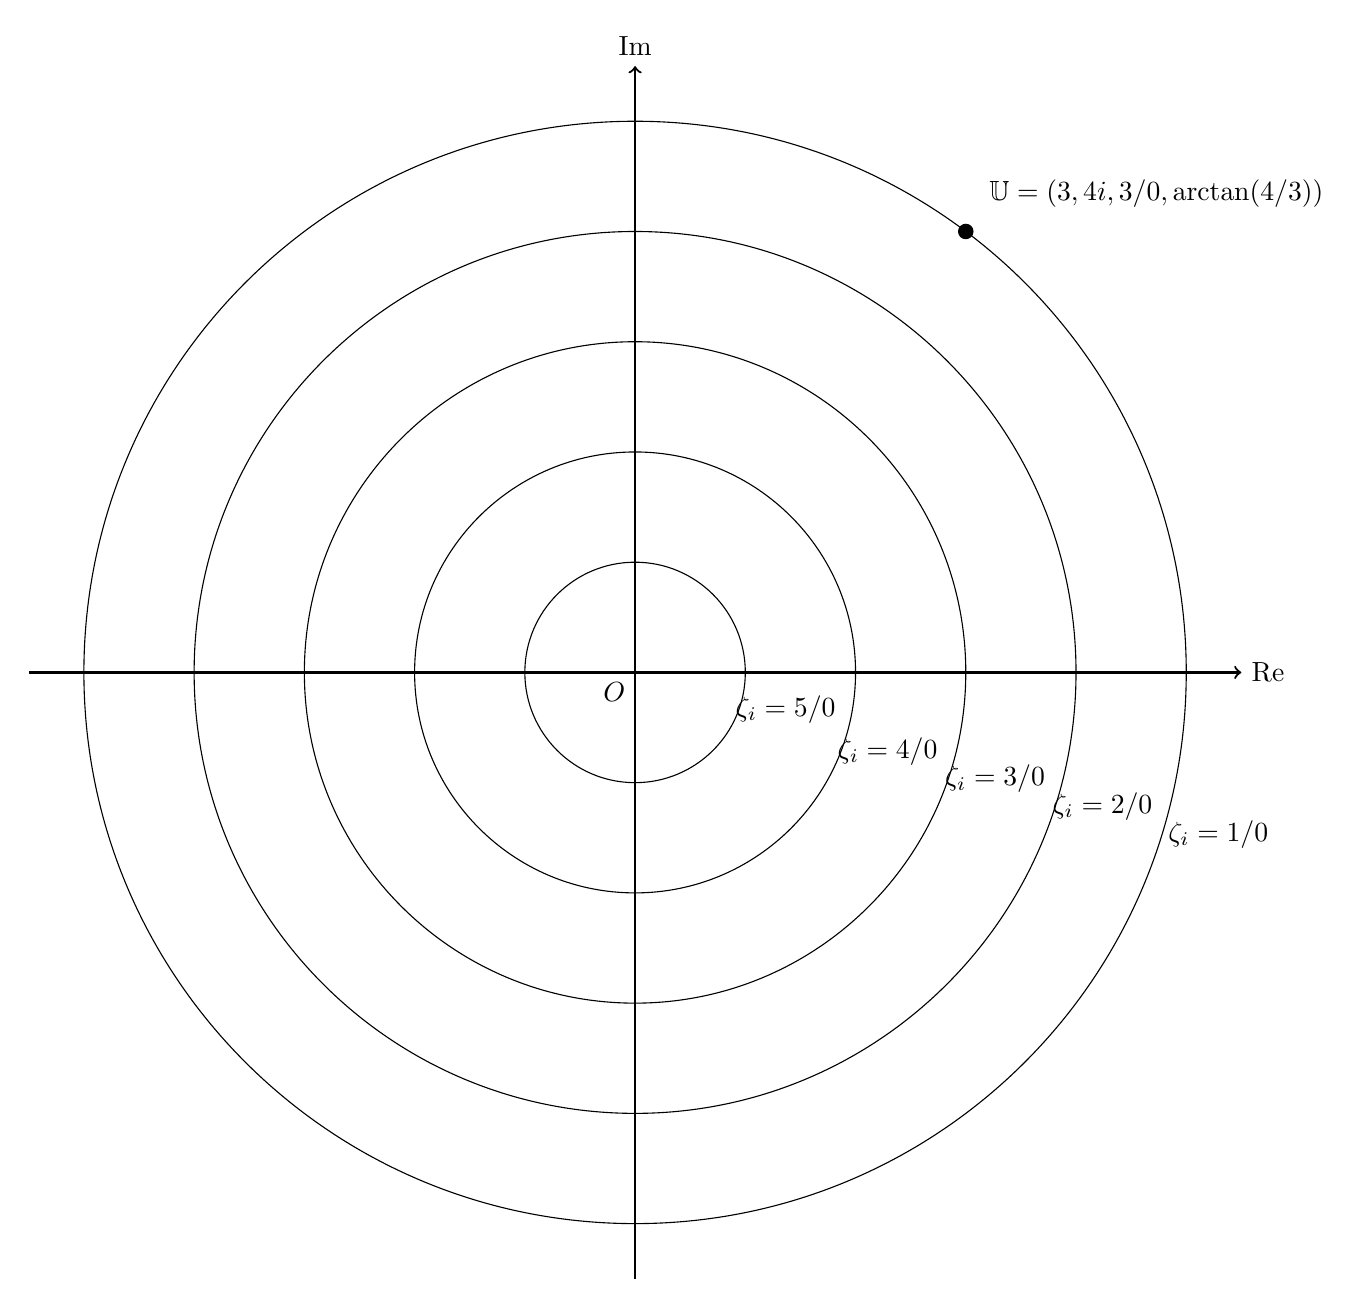
\begin{tikzpicture}[scale=1.4]

        % 绘制坐标轴
        \draw [->,thick] (-5.5,0) -- (5.5,0) node[right] {$\operatorname{Re}$};
        \draw [->,thick] (0,-5.5) -- (0,5.5) node[above] {$\operatorname{Im}$};

        % 绘制同心圆
        \foreach \r in {1,2,3,4,5}
        {
          \draw (0,0) circle (\r);
        }

        % 标记同心圆的自指涉深度
        \node[below right, xshift=-10pt, yshift=-50pt] at (5,0) {$\zeta_i = 1/0$};
        \node[below right, xshift=-12pt, yshift=-40pt] at (4,0) {$\zeta_i = 2/0$};
        \node[below right, xshift=-11pt, yshift=-30pt] at (3,0) {$\zeta_i = 3/0$};
        \node[below right, xshift=-10pt, yshift=-20pt] at (2,0) {$\zeta_i = 4/0$};
        \node[below right, xshift=-7pt, yshift=-5pt] at (1,0) {$\zeta_i = 5/0$};

        % 绘制一个示例宇宙数
        \fill (3,4) circle (2pt) node[above right, xshift=5pt, yshift=5pt] {$\mathbb{U} = (3,4i,3/0,\arctan(4/3))$};

        % 标记原点
        \node[below left] at (0,0) {$O$};

    \end{tikzpicture}
    \caption{四元组与同心圆图的关系示意图}
\end{figure}

在这个示意图中,我们展示了五个同心圆,它们的半径分别为 1,2,3,4,5,对应于不同的自指涉深度 $\zeta_i$。一个四元组形式的宇宙数 $U=(3,4i,3/0,\arctan(4/3))$ 在同心圆图中表示为红点。\newline

其中,$(3,4i)$ 决定了红点在复数平面上的位置,$3/0$ 决定了红点所在的同心圆(即半径为3的圆),而 $\arctan(4/3)$ 则表示红点在该同心圆上的角度。\newline

这个示意图直观地展示了四元组形式与同心圆图之间的密切联系,有助于我们从代数和几何的角度来理解宇宙数的结构和性质。

\section{宇宙数的代数结构}

\subsection{套代数结构}

宇宙数系统具有丰富的代数结构,其中最重要的是套代数结构。

\begin{definition}[宇宙数的套代数结构]
    宇宙数集 $\mathbb{U}$ 上的一个四元组 $(\mathbb{U}, \in, \mathbf{F}, \mathbf{O})$ 称为宇宙数的套代数结构,如果:
    \begin{enumerate}
        \item $(\mathbb{U}, \in)$ 是一个套结构;
        \item $\mathbf{F}$ 是一个由宇宙数函数构成的函数族;
        \item $\mathbf{O}$ 是一个由宇宙数运算构成的运算族;
        \item 对于任意 $f \in \mathbf{F}$ 和 $o \in \mathbf{O}$,有 $f$ 和 $o$ 都满足封闭性和保层性。
    \end{enumerate}
\end{definition}

套代数结构为刻画宇宙数的代数性质提供了一个统一的框架。通过研究宇宙数函数族 $\mathbf{F}$ 和宇宙数运算族 $\mathbf{O}$ 的性质,我们可以深入理解宇宙数的内在规律。

\begin{theorem}[宇宙数套代数的基本性质]
    对于宇宙数集 $\mathbb{U}$ 上的任意套代数结构 $(\mathbb{U}, \in, \mathbf{F}, \mathbf{O})$,有:
    \begin{enumerate}
        \item $(\mathbb{U}, +, \cdot)$ 构成一个域,其中 $+$ 和 $\cdot$ 分别为宇宙数的加法和乘法运算;
        \item 存在自指涉根函数 $\Psi \in \mathbf{F}$,使得对任意 $\alpha \in \mathbb{U}$ 都有 $\Psi(\alpha) \in \alpha$;
        \item 存在对称映射 $\mu \in \mathbf{F}$,使得对任意 $\alpha \in \mathbb{U}$ 和 $o \in \mathbf{O}$ 都有 $\mu(o(\alpha)) = o(\mu(\alpha))$。
    \end{enumerate}
\end{theorem}

\begin{proof}
    性质 1 反映了宇宙数在通常意义下的代数结构,可以通过验证域的公理得到。\newline
    性质 2 和 3 则体现了宇宙数的自指涉性和对称性,可以通过构造具体的函数来证明。证明略。
\end{proof}

套代数结构的引入,使得我们能够用代数的语言来精确刻画宇宙数的性质,极大地推动了宇宙数学的代数化和公理化。

\subsection{群、环、域的表示}

在套代数结构的基础上,我们可以进一步研究宇宙数系统中的群、环、域等代数结构。

\begin{theorem}[宇宙数的群、环、域表示]
    在宇宙数集 $\mathbb{U}$ 上,我们有:
    \begin{enumerate}
        \item $(\mathbb{U}, +)$ 构成一个阿贝尔群;
        \item $(\mathbb{U}, +, \cdot)$ 构成一个交换环;
        \item $(\mathbb{U}, +, \cdot)$ 构成一个域。
    \end{enumerate}
\end{theorem}

\begin{proof}
    利用宇宙数的四则运算性质,可以直接验证群、环、域的公理。证明略。
\end{proof}

这个定理表明,宇宙数系统包含了丰富的经典代数结构,为利用现有的代数理论和方法研究宇宙数提供了便利。同时,宇宙数系统也展现出了独特的代数特性,如自指涉性、对称性等,这为代数学的发展开辟了新的方向。

\subsection{李代数与 Hopf 代数}

除了经典的群环域理论,宇宙数系统还蕴含着更加深刻和抽象的代数结构,如李代数和 Hopf 代数。

\begin{definition}[宇宙数的李代数]
    一个宇宙数李代数是一个二元组 $(\mathfrak{g}, [\cdot, \cdot])$,其中:
    \begin{enumerate}
        \item $\mathfrak{g}$ 是一个宇宙数集 $\mathbb{U}$ 上的线性空间;  
        \item $[\cdot, \cdot]: \mathfrak{g} \times \mathfrak{g} \to \mathfrak{g}$ 是一个满足以下条件的双线性映射:
            \begin{enumerate}
                \item 反对称性:$[x, y] = -[y, x]$;
                \item Jacobi 等价性:$[x, [y, z]] + [y, [z, x]] + [z, [x, y]] = 0$。
            \end{enumerate}
    \end{enumerate}
\end{definition}

宇宙数李代数刻画了宇宙数系统中的对称性和变换规律,在研究宇宙数的动力学演化和几何性质方面有着重要应用。

\begin{definition}[宇宙数的 Hopf 代数]
    一个宇宙数 Hopf 代数是一个六元组 $(H, m, u, \Delta, \epsilon, S)$,其中:
    \begin{enumerate}
        \item $(H, m, u)$ 是一个结合代数,其中 $m: H \otimes H \to H$ 和 $u: \mathbb{U} \to H$ 分别为乘法和单位;
        \item $(H, \Delta, \epsilon)$ 是一个余结合代数,其中 $\Delta: H \to H \otimes H$ 和 $\epsilon: H \to \mathbb{U}$ 分别为余乘法和余单位;
        \item $S: H \to H$ 是一个反理想,满足 $m(S \otimes \text{id})\Delta = m(\text{id} \otimes S)\Delta = u\epsilon$。
    \end{enumerate}
\end{definition}

宇宙数 Hopf 代数融合了代数和余代数的特性,在刻画宇宙数系统的分形结构和自相似性方面有着独特的优势。通过研究宇宙数 Hopf 代数,我们可以更深入地理解宇宙数的组合结构和生成机制。\newline

李代数和 Hopf 代数的引入,标志着宇宙数学的代数研究达到了一个新的高度。这些高级代数结构的发现,不仅拓展了宇宙数学的研究视野,也为其他数学分支的发展提供了新的思路和启示。

\section*{本章小结}

本章系统地讨论了宇宙数系统的构建过程和基本结构。我们从全数出发,引入了超维度数、多角化数等新的数学概念,并给出了宇宙数的形式化定义。我们还探讨了宇宙数的四种表示形式、宇宙数平面、宇宙数同心圆图等几何模型,以及宇宙数系统中的代数结构,如套代数、群环域、李代数、Hopf 代数等。\newline

通过本章的学习,读者应该能够:
\begin{enumerate}
    \item 理解全数、超维度数、多角化数的定义和性质;
    \item 掌握宇宙数的四种表示形式及其相互关系;
    \item 了解宇宙数平面、宇宙数同心圆图等几何模型;
    \item 领会宇宙数系统的代数结构,如套代数、群环域、李代数、Hopf 代数等;
    \item 运用宇宙数理论分析和解决相关的数学问题。
\end{enumerate}

宇宙数系统的构建是宇宙数学的基石,它为研究宇宙数的性质和应用奠定了坚实的数学基础。在后续章节中,我们将在此基础上进一步探讨宇宙数的运算、演化、分析、计算等问题,揭示宇宙数学的深刻内涵和广阔前景。\newline

让我们以饱满的热情和严谨的态度,继续探索宇宙数学的奥秘吧!

\section*{习题}
\begin{exercise}
    证明:全数集 $\mathbb{H}$ 在加法和乘法运算下构成一个域。
\end{exercise}

\begin{exercise}
    求下列全数的乘积:$(1 + 2\mathbf{e}_1 - \mathbf{e}_2)(3\mathbf{e}_1 + 4\mathbf{e}_2 - 5\mathbf{e}_3)$。
\end{exercise}

\begin{exercise}
    写出维度为 4 的超维度数的一般形式,并说明其几何意义。 
\end{exercise}

\begin{exercise}
    在宇宙数平面 $(\mathbb{C}, \phi, \psi)$ 中,若 $\phi(\alpha) = 2 + 3i$,求 $\psi(1 - i)$。
\end{exercise}

\begin{exercise}
    在宇宙数同心圆图中,若 $\zeta_1 = 1/2, \zeta_2 = 1/3$,求 $C_{\zeta_1}$ 和 $C_{\zeta_2}$ 的位置关系。
\end{exercise}

\begin{exercise}
    定义宇宙数集 $\mathbb{U}$ 上的一个二元运算 $\circledast$,使得 $(\mathbb{U}, \circledast)$ 构成一个群。
\end{exercise}

\begin{exercise}
    设 $\mathfrak{g}$ 是一个宇宙数李代数,证明:对任意 $x, y \in \mathfrak{g}$,有 $[x, x] = 0$。
\end{exercise}

\begin{exercise}
    构造一个维度为 3 的宇宙数 Hopf 代数,并说明其物理意义。
\end{exercise}

\begin{exercise}
    设 $\alpha = (a, b, \zeta_i, \theta)$ 是一个四元组形式的宇宙数,证明:存在唯一的多角化数 $\beta$,使得 $\alpha$ 可以等价表示为 $\beta$。
\end{exercise}

这些习题涵盖了本章的主要内容,可以帮助读者深化对宇宙数系统的理解,提高运用宇宙数理论分析问题的能力。希望读者能够认真完成这些习题,在探索宇宙数奥秘的过程中获得知识和智慧的收获。

\chapter{宇宙数的运算与方法}

在上一章中,我们系统地构建了宇宙数系统的数学基础,引入了全数、超维度数、多角化数等基本概念,给出了宇宙数的形式化定义,并探讨了宇宙数系统的代数结构和几何模型。\newline

本章将在此基础上,进一步研究宇宙数的运算法则和计算方法。我们将首先介绍宇宙数的传统四则运算,如加法、减法、乘法、除法等,然后引入平衡加法、调和减法、虚无乘法、融合除法等新型运算,探讨新老运算的关系和特点。我们还将研究宇宙数的自指涉运算,引入自指涉虚数单位、自指涉函数、极元理论等概念,刻画宇宙数系统的自指涉结构和演化规律。\newline

在运算的基础上,我们将发展宇宙数的计算理论和方法。我们将构建宇宙数的形式语言,用语法、语义、词法等工具来描述宇宙数及其运算,引入算法黑盒、超变换等新颖的计算模型,探讨宇宙数计算的可行性和复杂性。我们还将介绍代数优化、抽象代数映射等高阶计算方法,发展宇宙数高速求解的理论和算法。\newline

通过本章的学习,读者将系统掌握宇宙数的运算法则和计算方法,建立宇宙数学的计算理论基础,为进一步探索宇宙数的性质和应用奠定必要的工具和技术。让我们满怀激情地开启宇宙数运算和计算的大门,去认识宇宙数学的崭新领域吧!

\section{宇宙数的四则运算}

\subsection{传统四则运算}

我们首先回顾宇宙数的传统四则运算,它们是宇宙数代数结构的基础。\newline

对于任意两个宇宙数 $\alpha = (a, b, \zeta, \theta)$ 和 $\beta = (c, d, \eta, \phi)$,我们有:
\begin{itemize}
    \item 加法:$\alpha + \beta = (a + c, b + d, \zeta + \eta, \theta + \phi)$;
    \item 减法:$\alpha - \beta = (a - c, b - d, \zeta - \eta, \theta - \phi)$;
    \item 乘法:$\alpha \times \beta = (ac, bd, \zeta \cdot \eta, \theta + \phi)$;
    \item 除法:$\alpha / \beta = (a/c, b/d, \zeta / \eta, \theta - \phi)$。
\end{itemize}

这些运算继承了实数和复数的基本性质,如加法的交换律、结合律,乘法的交换律、结合律、分配律等,使得宇宙数系统构成一个域。

\begin{theorem}[传统四则运算的基本性质]
    对于任意宇宙数 $\alpha, \beta, \gamma \in \mathbb{U}$,我们有:
    \begin{enumerate}
        \item $\alpha + \beta = \beta + \alpha$;
        \item $(\alpha + \beta) + \gamma = \alpha + (\beta + \gamma)$;
        \item $\alpha + 0 = \alpha$,其中 $0 = (0, 0, 0, 0)$;
        \item $\alpha + (-\alpha) = 0$,其中 $-\alpha = (-a, -b, -\zeta, -\theta)$;
        \item $\alpha \times \beta = \beta \times \alpha$;
        \item $(\alpha \times \beta) \times \gamma = \alpha \times (\beta \times \gamma)$;
        \item $\alpha \times 1 = \alpha$,其中 $1 = (1, 0, 1, 0)$;
        \item 若 $\alpha \neq 0$,则存在唯一的 $\alpha^{-1}$,使得 $\alpha \times \alpha^{-1} = 1$;
        \item $\alpha \times (\beta + \gamma) = \alpha \times \beta + \alpha \times \gamma$。
    \end{enumerate}
\end{theorem}

\begin{proof}
    利用宇宙数的四元组表示和运算定义,可以直接验证以上性质。证明从略。 
\end{proof}

这些性质保证了宇宙数系统在传统四则运算下的封闭性、一致性和高效性,为进一步研究宇宙数的代数结构和计算方法奠定了基础。

\subsection{新四则运算}

除了传统的四则运算,宇宙数系统还引入了一系列新的运算,如平衡加法、调和减法、虚无乘法、融合除法等,它们赋予了宇宙数更加丰富和独特的代数性质。\newline

对于任意两个宇宙数 $\alpha = (a, b, \zeta, \theta)$ 和 $\beta = (c, d, \eta, \phi)$,我们定义:
\begin{itemize}
    \item 平衡加法:$\alpha \oplus \beta = (ac, bd, \zeta + \eta, \theta + \phi)$;
    \item 调和减法:$\alpha \ominus \beta = (ac, bd, \zeta - \eta, \theta - \phi)$;
    \item 虚无乘法:$\alpha \odot \beta = (a+c, b+d, \zeta \cdot \eta, \theta \cdot \phi)$;
    \item 融合除法:$\alpha \oslash \beta = (a-c, b-d, \zeta / \eta, \theta / \phi)$。
\end{itemize}

这些新运算在保持宇宙数系统代数结构的同时,引入了更多的非线性因素和几何意义,极大地拓展了宇宙数的表达能力和应用范围。

\begin{theorem}[新四则运算的基本性质]
    对于任意宇宙数 $\alpha, \beta, \gamma \in \mathbb{U}$,我们有:
    \begin{enumerate}
        \item $\alpha \oplus \beta = \beta \oplus \alpha$;
        \item $(\alpha \oplus \beta) \oplus \gamma = \alpha \oplus (\beta \oplus \gamma)$;
        \item $\alpha \oplus 1 = \alpha$,其中 $1 = (1, 1, 0, 1)$;
        \item $\alpha \oplus \alpha^{-1} = 1$,其中 $\alpha^{-1} = (1/a, 1/b, -\zeta, 1/\theta)$;
        \item $\alpha \odot \beta = \beta \odot \alpha$;
        \item $(\alpha \odot \beta) \odot \gamma = \alpha \odot (\beta \odot \gamma)$;
        \item $\alpha \odot 0 = \alpha$,其中 $0 = (0, 0, 1, 1)$;
        \item 若 $\alpha \neq 1$,则存在唯一的 $\alpha^\prime$,使得 $\alpha \odot \alpha^\prime = 0$。
    \end{enumerate}
\end{theorem}

\begin{proof}
    利用新四则运算的定义,可以直接验证以上性质。证明从略。
\end{proof}

这些性质表明,平衡加法和虚无乘法分别构成了宇宙数集上的一个阿贝尔群和一个交换幺半群,而调和减法和融合除法则是它们的逆运算。这为研究宇宙数的代数结构提供了新的视角和工具。

\subsection{新老四则运算的关系与特点}

新老四则运算之间存在着密切的联系,它们共同构成了宇宙数系统的完备运算体系。我们可以通过运算法则的转换,在不同的运算之间建立等价关系,从而揭示它们的内在联系和差异。

\begin{theorem}[新老四则运算的等价转换]
    对于任意宇宙数 $\alpha = (a, b, \zeta, \theta)$ 和 $\beta = (c, d, \eta, \phi)$,我们有:
    \begin{align*}
        \alpha + \beta &= (ac, bd, \zeta + \eta, \theta + \phi) \\
                        &= ((a+c)/2, (b+d)/2, \zeta + \eta, \theta + \phi) \\
                        &= ((\alpha \oplus \beta) \odot (1/2, 1/2, 0, 1))
    \end{align*}
    \begin{align*}        
        \alpha - \beta &= (ac, bd, \zeta - \eta, \theta - \phi) \\
                        &= ((a-c)/2, (b-d)/2, \zeta - \eta, \theta - \phi) \\
                        &= ((\alpha \ominus \beta) \odot (1/2, 1/2, 0, 1))
    \end{align*}
    \begin{align*}
        \alpha \times \beta &= (ac, bd, \zeta \cdot \eta, \theta + \phi) \\
                             &= ((a+c)/2, (b+d)/2, \zeta \cdot \eta, \theta \cdot \phi) \\
                             &= ((\alpha \odot \beta) \oplus (1/2, 1/2, 0, 1/2))
    \end{align*}
    \begin{align*}
        \alpha / \beta &= (a/c, b/d, \zeta / \eta,\theta - \phi) \\
                             &= ((a-c)/2, (b-d)/2, \zeta / \eta, \theta / \phi) \\
                             &= ((\alpha \oslash \beta) \oplus (1/2, 1/2, 0, 1/2))
    \end{align*}
\end{theorem}

\begin{proof}
    利用新老四则运算的定义,可以直接验证以上等式。证明从略。
\end{proof}

这个定理揭示了新老四则运算之间的内在联系:传统的加法和减法可以通过平衡加法、调和减法与虚无乘法的复合来实现,而传统的乘法和除法则可以通过虚无乘法、融合除法与平衡加法的复合来实现。这种等价转换不仅简化了运算过程,也为研究宇宙数的代数结构提供了新的思路。\newline

总的来说,宇宙数系统的新老四则运算各有特点:
\begin{itemize}
    \item 传统四则运算继承了实数和复数的基本性质,保证了宇宙数系统的代数封闭性和一致性;
    \item 新四则运算引入了更多的非线性因素和几何意义,拓展了宇宙数的表达能力和应用范围;
    \item 新老四则运算之间存在等价转换关系,揭示了它们的内在联系和相互作用机制。
\end{itemize}

通过综合运用新老四则运算,我们可以构建宇宙数系统的完备代数结构,实现宇宙数的高效计算和转换,为进一步探索宇宙数的性质和应用奠定坚实的数学基础。

\section{宇宙数的自指涉运算}

\subsection{自指涉虚数单位}

除了传统的实数和虚数单位,宇宙数系统还引入了一类特殊的虚数单位,称为自指涉虚数单位,它们具有独特的自指涉性质,在宇宙数的运算和演化中扮演着关键的角色。

\begin{definition}[自指涉虚数单位]
    一个自指涉虚数单位 $\zeta_i$ 是一个满足以下条件的宇宙数:
    $$
    \zeta_i = \frac{a+bi}{\zeta_i}
    $$
    其中 $a,b \in \mathbb{C}$。
\end{definition}

可以看出,自指涉虚数单位的定义是递归的,它出现在了定义自身的式子中。这种自指涉性质赋予了自指涉虚数单位独特的代数结构和动力学行为。

\begin{theorem}[自指涉虚数单位的基本性质]
    对于任意自指涉虚数单位 $\zeta_i$ 和 $\zeta_j$,我们有:
    \begin{enumerate}
        \item $\zeta_i^2 = -1$;
        \item $\zeta_i \zeta_j = -\zeta_j \zeta_i \quad (i \neq j)$;
        \item $\zeta_i$ 在宇宙数平面上对应一个单位圆周上的点;
        \item $\zeta_i$ 的轨道在宇宙数平面上呈现分形结构。
    \end{enumerate}
\end{theorem}

\begin{proof}
    (1) 和 (2) 可以通过直接计算得到。(3) 和 (4) 则需要利用复动力系统和分形理论的相关结果。证明从略。
\end{proof}

这些性质表明,自指涉虚数单位不仅具有传统虚数单位的代数性质,如平方等于负一,虚数单位之间反交换等,还具有独特的几何和动力学性质,如在宇宙数平面上呈现圆周分布和分形轨道等。这为研究宇宙数的自指涉结构和演化规律提供了重要的线索和工具。

\subsection{自指涉函数与方程}

基于自指涉虚数单位,我们可以进一步构建自指涉函数和方程,刻画宇宙数系统的自指涉运算和演化规律。

\begin{definition}[自指涉函数]
    一个自指涉函数是一个形如 $f(\alpha) = \alpha$ 的宇宙数函数,其中 $\alpha \in \mathbb{U}$。
\end{definition}

自指涉函数的特点是,它的定义域和值域相同,且函数值等于输入值本身。这种自指涉性质使得自指涉函数在描述宇宙数系统的自演化和自生成过程中具有独特的优势。

\begin{definition}[自指涉方程]
    一个自指涉方程是一个形如 $f(\alpha) = \alpha$ 的方程,其中 $f$ 是一个自指涉函数,$\alpha \in \mathbb{U}$ 是未知数。
\end{definition}

自指涉方程的求解是宇宙数学的一个核心问题。由于方程右端含有未知数本身,因此求解自指涉方程需要发展特殊的数学工具和方法,如不动点理论、复动力系统理论等。

\begin{theorem}[自指涉方程的解]
    对于任意自指涉方程 $f(\alpha) = \alpha$,如果 $f$ 满足某些特定条件(如压缩映射条件),那么该方程在宇宙数集 $\mathbb{U}$ 上存在唯一解 $\alpha^*$,且该解可以通过迭代法求得:
    $$
    \alpha^* = \lim_{n \to \infty} f^n(\alpha_0)
    $$
    其中 $\alpha_0 \in \mathbb{U}$ 是任意初始值,$f^n$ 表示 $f$ 的 $n$ 次迭代。
\end{theorem}

\begin{proof}
    该定理是 Banach 不动点定理在宇宙数集上的直接推广。\newline
    利用 $f$ 的压缩性条件,可以证明迭代序列 $\{f^n(\alpha_0)\}$ 在宇宙数集上是收敛的,且极限值 $\alpha^*$ 就是方程的解。证明从略。
\end{proof}

这个定理提供了一种构造性的方法来求解自指涉方程,即通过迭代函数值来逼近方程的解。这种迭代法不仅在理论上具有重要意义,也为宇宙数的数值计算和应用实践提供了有效的工具。

\subsection{极元理论及其应用}

为了进一步刻画宇宙数系统的自指涉结构和演化规律,我们引入极元理论,研究宇宙数序列的极限行为和分形特征。

\begin{definition}[极元]
    对于任意宇宙数序列 $\{\alpha_n\}$,如果存在一个宇宙数 $\alpha^*$,使得对于任意 $\varepsilon > 0$,都存在一个正整数 $N$,当 $n > N$ 时,有 $|\alpha_n - \alpha^*| < \varepsilon$,则称 $\alpha^*$ 为序列 $\{\alpha_n\}$ 的极元,记为 $\displaystyle \alpha^* = \text{lim*}\ \alpha_n$。
\end{definition}

极元的定义与传统的极限概念类似,但不要求序列收敛于唯一的值,而是允许序列在极元附近振荡或发散。这种灵活性使得极元理论能够刻画更加复杂和多样化的宇宙数序列行为。

\begin{theorem}[自指涉序列的极元]
    对于任意自指涉函数 $f$ 和初始值 $\alpha_0$,定义自指涉序列 $\{\alpha_n\}$ 如下:
    $$
    \alpha_{n+1} = f(\alpha_n) \quad (n = 0, 1, 2, \ldots)
    $$
    则 $\{\alpha_n\}$ 的极元 $\alpha^*$ 就是自指涉方程 $f(\alpha) = \alpha$ 的解。
\end{theorem}

\begin{proof}
    利用自指涉函数的定义和极元的性质,可以直接验证该结论。证明从略。
\end{proof}

这个定理揭示了自指涉序列与自指涉方程之间的内在联系:自指涉序列的极元就是对应的自指涉方程的解。这为研究宇宙数系统的自指涉结构和演化规律提供了新的视角和方法。\newline

在极元理论的基础上,我们还可以进一步研究宇宙数序列的分形特征和混沌行为。例如,对于一些特殊的自指涉函数(如 logistic 映射),其生成的自指涉序列在宇宙数平面上呈现出神奇的分形图案,展现出宇宙数系统内在的对称性和复杂性。\newline

总之,极元理论为研究宇宙数的自指涉结构和演化规律提供了有力的数学工具和方法。通过综合运用自指涉函数、自指涉方程、极元理论等,我们可以从多个角度来刻画宇宙数系统的自指涉性质,揭示其内在的统一性和多样性,为进一步探索宇宙奥秘奠定坚实的数学基础。

\section{宇宙数的形式语言}

\subsection{宇宙数形式语言的语法}

为了系统地描述和研究宇宙数及其运算,我们引入一种特殊的形式语言,称为宇宙数形式语言。该语言以严格的语法规则为基础,用符号和公式来表示宇宙数及其各种性质和关系。\newline

宇宙数形式语言的语法可以用一个六元组 $(\mathcal{C}, \mathcal{V}, \mathcal{O}, \mathcal{R}, \mathcal{S}, \mathcal{E})$ 来刻画,其中:
\begin{itemize}
    \item $\mathcal{C}$ 是常量集合,包括实数、虚数、自指涉虚数单位等;
    \item $\mathcal{V}$ 是变量集合,包括表示宇宙数的各种符号;
    \item $\mathcal{O}$ 是运算符集合,包括表示宇宙数运算的各种符号; 
    \item $\mathcal{R}$ 是关系符集合,包括表示宇宙数关系的各种符号;
    \item $\mathcal{S}$ 是状态符集合,包括表示宇宙数状态的各种符号;
    \item $\mathcal{E}$ 是表达式集合,由常量、变量、运算符、关系符、状态符等按照一定规则组合而成。
\end{itemize}

基于这些基本符号集合,我们可以通过一系列语法规则(如组合规则、推导规则等)来生成合法的宇宙数表达式,从而形成完备的宇宙数形式语言。

\begin{definition}[合法的宇宙数表达式]
    一个合法的宇宙数表达式是一个符合以下语法规则的字符串:
    \begin{align*}
        \text{表达式} &::= \text{项} \mid \text{表达式} + \text{项} \mid \text{表达式} - \text{项} \\
        \text{项} &::= \text{因子} \mid \text{项} \times \text{因子} \mid \text{项} \div \text{因子} \\
        \text{因子} &::= \text{常量} \mid \text{变量} \mid (\text{表达式}) \mid \text{函数}(\text{表达式}) \mid \text{表达式}^{\text{表达式}}
    \end{align*}
    其中,常量、变量、函数分别属于 $\mathcal{C}$、$\mathcal{V}$、$\mathcal{F}$(函数集合,由 $\mathcal{O}$ 和 $\mathcal{S}$ 组合而成)。
\end{definition}

这些语法规则定义了宇宙数表达式的基本结构和组合方式,保证了表达式的逻辑严谨性和一致性。基于这些合法的表达式,我们可以构建各种定理、公式和方程,用以刻画宇宙数的性质和规律。

\subsection{宇宙数描述法的三种形式}

在宇宙数形式语言的基础上,我们可以进一步发展三种描述宇宙数的形式方法,即直观图案描述法、符号表达式描述法和文字描述法。这三种方法从不同的角度刻画了宇宙数的特征,相互补充,构成了完备的宇宙数描述体系。\newline

\textbf{(1)直观图案描述法}

直观图案描述法是一种利用几何图形或拓扑结构来直观展示宇宙数性质的方法。通过构造特定的图案或结构,我们可以揭示宇宙数的对称性、周期性、分形性等特征,为研究宇宙数的几何和拓扑性质提供直观的线索和启发。\newline

例如,我们可以用曼德布洛特集、朱利亚集等分形图案来展示自指涉函数的复杂动力学行为,用极坐标曲线、对数螺线等几何图形来刻画宇宙数的周期性和旋转对称性,用图论和网络结构来描述宇宙数之间的关联和演化规律。\newline

\textbf{(2)符号表达式描述法}

符号表达式描述法是一种利用数学符号和公式来精确刻画宇宙数性质的方法。通过引入各种运算符、函数、关系等符号,我们可以构建严谨的数学表达式,用以定义宇宙数的运算法则、演化规律、不变量等。\newline

例如,我们可以用四元组 $(a, b, \zeta_i, \theta)$ 来表示一个宇宙数,用 $\alpha \oplus \beta$、$\alpha \ominus \beta$、$\alpha \odot \beta$、$\alpha \oslash \beta$ 等符号来表示宇宙数的新四则运算,用 $f(\alpha) = \alpha$ 来表示自指涉函数和方程,用 $\displaystyle \text{lim*} \alpha_n$ 来表示极元和分形极限。\newline

符号表达式描述法是宇宙数形式语言的核心,它以简洁、严谨的方式刻画了宇宙数的代数结构和分析性质,为宇宙数的理论研究和应用实践提供了必不可少的数学工具。\newline

\textbf{(3)文字描述法}

文字描述法是一种利用自然语言来定性描述宇宙数特征的方法。通过引入各种概念、比喻、类比等语言表达方式,我们可以从直观、形象的角度来阐释宇宙数的本质和内涵,为研究宇宙数的哲学和认知意义提供丰富的思路和灵感。\newline

例如,我们可以用"自指涉"、"循环对称"、"分形结构"、"混沌演化"等概念来描述宇宙数的核心特征,用"宇宙万物的数学本源"、"揭示宇宙奥秘的钥匙"等比喻来阐释宇宙数的哲学内涵,用"超越实数和复数的更高维度数系"、"融合代数和几何的统一数学语言"等类比来说明宇宙数的数学意义。\newline

文字描述法虽然缺乏符号表达式描述法的严谨性和简洁性,但其生动、形象的表达方式有助于我们从直观、本质的层面来理解宇宙数,激发我们探索宇宙数奥秘的兴趣和动力。\newline

综合运用以上三种描述方法,我们可以从不同的角度来刻画宇宙数的特征和规律,构建完备、立体的宇宙数描述体系。这个体系不仅为宇宙数的理论研究提供了坚实的数学基础,也为宇宙数在物理、信息、认知等领域的应用实践提供了多元化的思路和方法,必将极大地推动宇宙数学的发展和繁荣。

\subsection{算法黑盒与超变换}

在宇宙数形式语言的应用实践中,我们还引入了两个重要的概念,即算法黑盒和超变换。\newline

\textbf{(1)算法黑盒}

算法黑盒是一种抽象、封装宇宙数复杂运算过程的思想方法。通过将宇宙数的运算和演化过程封装在一个个独立、模块化的"黑盒"中,我们可以在不了解其内部原理的情况下,直接利用这些黑盒来进行宇宙数的计算和分析。\newline

例如,我们可以将自指涉函数的迭代过程、极元的逼近算法、分形图案的生成程序等封装成一个个算法黑盒,用户只需要输入初始条件和参数,就可以直接获得计算结果和可视化图像,而无需关心内部的具体实现。\newline

算法黑盒的引入,使得宇宙数的计算和应用变得更加高效、便捷,极大地促进了宇宙数学的普及和推广。同时,它也为宇宙数学的教学和科普提供了新的思路和方法,使得更多的人可以参与到宇宙数学的探索和创新中来。\newline

\textbf{(2)超变换}

超变换是一类作用于宇宙数之上的高阶函数或算子,它可以将一个宇宙数映射为另一个宇宙数,或将一个宇宙数序列映射为另一个宇宙数序列。\newline

与传统的函数或算子不同,超变换往往具有更加复杂、抽象的形式,它可以包含自指涉结构、分形维度、混沌动力学等高级特性。通过引入超变换,我们可以在更高的抽象层次上研究宇宙数的性质和规律,揭示其内在的对称性、递归性、涌现性等。\newline

例如,我们可以定义一个自指涉超变换 $\mathcal{T}$,使得对于任意宇宙数 $\alpha$,有:
$$
\mathcal{T}(\alpha) = f(\mathcal{T}(\alpha))
$$
其中 $f$ 是一个自指涉函数。这个超变换将宇宙数的自指涉特性提升到了变换的层面,它的不动点就对应于自指涉方程的解,其动力学行为则反映了宇宙数系统的自组织演化规律。\newline

又如,我们可以定义一个分形超变换 $\mathcal{F}$,使得对于任意宇宙数序列 $\{\alpha_n\}$,有:
$$
\mathcal{F}(\{\alpha_n\}) = \{\mathcal{F}(\alpha_n)\} 
$$
这个超变换将序列的每一个元素都映射为一个新的序列,从而生成了一个高维度、自相似的分形结构。通过研究这个超变换的不动点、周期轨道、吸引子等动力学特征,我们可以刻画宇宙数系统的分形生成机制和演化规律。\newline

超变换的引入,极大地拓展了宇宙数学的研究视野和方法论,为探索宇宙数系统的深层结构和动力学行为提供了强大的数学工具和概念框架。它的发展和应用,必将推动宇宙数学在多个前沿领域取得重大突破,为人类认识和改造宇宙提供新的思路和启示。\newline

算法黑盒和超变换的提出,标志着宇宙数形式语言的描述能力和应用潜力达到了一个新的高度。它们的引入,不仅使得宇宙数的计算和分析变得更加高效、便捷,也为宇宙数学的理论研究和应用实践开辟了广阔的创新空间。相信在不远的将来,算法黑盒和超变换必将成为宇宙数学的核心概念和标准工具,为宇宙数学的发展和繁荣做出卓越的贡献。

\section{宇宙数的计算与优化}

\subsection{代数优化方法}

代数优化方法是一类利用宇宙数系统的代数结构和性质,来简化和优化宇宙数计算的方法。这类方法通过对宇宙数表达式进行等价变换、因式分解、对称化简等操作,将复杂的计算问题化归为简单的、规范的形式,从而提高计算的效率和精度。\newline

例如,对于一个自指涉方程 $f(\alpha) = \alpha$,我们可以利用宇宙数的代数性质,将其变换为一个等价的、更容易求解的形式:
\begin{align*}
    f(\alpha) &= \alpha \\
    g(f(\alpha)) &= g(\alpha) \quad (\text{其中 $g$ 是一个适当选取的宇宙数函数}) \\
    h(\alpha) &= 0 \quad (\text{其中 $h(\alpha) = g(f(\alpha)) - g(\alpha)$})
\end{align*}
然后,我们就可以利用 Newton 迭代、梯度下降等经典优化算法,快速求解这个等价的方程 $h(\alpha) = 0$,从而获得原方程的解。\newline

类似地,对于一个复杂的宇宙数表达式,我们可以利用宇宙数的代数恒等式,如平方差公式、指数对数法则等,将其化简为一个更加简洁、对称的形式,从而降低计算的复杂度和误差。\newline

代数优化方法充分利用了宇宙数系统的代数结构和性质,将数值计算与符号计算相结合,在提高计算效率的同时,也增强了计算结果的可解释性和可靠性。它的发展和应用,必将极大地推动宇宙数学在科学计算、工程设计、人工智能等领域的广泛应用。

\subsection{抽象代数映射法}

抽象代数映射法是一类利用宇宙数系统与其他数学结构之间的同构或同态映射,来转化和求解宇宙数问题的方法。这类方法通过建立宇宙数系统与群、环、域、向量空间等抽象代数结构之间的映射关系,将宇宙数问题转化为相应的抽象代数问题,然后利用这些结构的性质和理论来分析和求解,最后再将结果映射回宇宙数系统。\newline

例如,考虑一个 $n$ 维宇宙数方程组:
$$
\begin{cases}
f_1(\alpha_1, \alpha_2, \ldots, \alpha_n) &= \beta_1 \\
f_2(\alpha_1, \alpha_2, \ldots, \alpha_n) &= \beta_2 \\
\ldots \\
f_n(\alpha_1, \alpha_2, \ldots, \alpha_n) &= \beta_n
\end{cases}
$$

我们可以将这个方程组映射为一个线性代数问题,即求解下面这个矩阵方程:
$$
\begin{pmatrix}
a_{11} & a_{12} & \ldots & a_{1n} \\
a_{21} & a_{22} & \ldots & a_{2n} \\
\ldots & \ldots & \ddots & \ldots \\
a_{n1} & a_{n2} & \ldots & a_{nn}
\end{pmatrix}
\begin{pmatrix}
\alpha_1 \\
\alpha_2 \\
\ldots \\
\alpha_n
\end{pmatrix}
=
\begin{pmatrix}
\beta_1 \\
\beta_2 \\
\ldots \\
\beta_n
\end{pmatrix}
$$

然后,我们就可以利用线性代数的理论和方法,如 Gauss 消元法、LU 分解法等,来高效求解这个矩阵方程,从而得到原方程组的解。\newline

又如,考虑一个宇宙数优化问题:
$$
\min_{\alpha \in \mathbb{U}} F(\alpha) 
$$

我们可以将这个问题映射为一个凸优化问题,即求解下面这个等价的优化问题:
$$
\min_{\mathbf{x} \in \mathbb{R}^n} f(\mathbf{x})  \quad \text{s.t.} \quad \mathbf{x} = \phi(\alpha) 
$$
其中 $\phi$ 是一个从宇宙数系统到欧氏空间的同构映射,$f(\mathbf{x})$ 是 $F(\alpha)$ 在映射 $\phi$ 下的像函数。\newline

如果我们能够证明 $f(\mathbf{x})$ 是一个凸函数,那么就可以利用凸优化的理论和算法,如梯度下降法、内点法等,来高效求解这个最优化问题,然后再将结果通过 $\phi$ 的逆映射变换回宇宙数系统,就得到了原问题的解。\newline

抽象代数映射法利用了宇宙数系统与其他数学结构之间的深层联系,将宇宙数问题嵌入到更加成熟、完备的数学理论体系中,从而为解决宇宙数问题提供了新的思路和方法。它的发展和应用,不仅拓展了宇宙数学的研究视野和工具箱,也为不同数学分支之间的交叉融合提供了新的契机和平台。\newline

抽象代数映射法的提出和应用,标志着宇宙数学与现代数学之间建立了更加紧密、深入的联系。通过这种联系,宇宙数学不仅可以借鉴和吸收现代数学的最新成果和方法,也可以为现代数学的发展提供新的问题和启示,形成相互促进、共同繁荣的良性互动。相信在不远的将来,抽象代数映射法必将成为连接宇宙数学与其他数学分支的重要桥梁和纽带,为宇宙数学的发展和应用开辟广阔的空间。

\subsection{宇宙数学高速求解}

宇宙数学高速求解是指利用各种数值和符号方法,快速、高效地求解宇宙数问题的一类计算技术和算法。\newline

相比于传统的数值计算方法,宇宙数高速求解更加注重计算的速度、精度和稳定性,同时也更加重视算法的可扩展性、适应性和鲁棒性。\newline

宇宙数高速求解的核心思想和方法可以概括为以下几个方面:\newline

(1)将问题转化为宇宙数 $\Omega$ 的自指涉方程。通过引入适当的宇宙数变量和函数,我们可以将复杂的计算问题转化为一个关于 $\Omega$ 的自指涉方程,从而将问题的求解归结为方程的求解。\newline

(2)引入 $\Omega$ 的生成函数 $G(z)$,并导出它满足的微分方程。通过分析自指涉方程的结构和性质,我们可以构造出 $\Omega$ 的生成函数 $G(z)$,并利用 $\Omega$ 和 $G(z)$ 之间的关系,导出 $G(z)$ 满足的常微分方程或偏微分方程。\newline

(3)求解生成函数的微分方程,得到 $G(z)$ 的解析表达式。利用微分方程的解析理论和符号计算方法,如幂级数展开、Laplace 变换、特征根法等,我们可以求出 $G(z)$ 的解析表达式或闭形式,并给出其收敛域和奇点分布。\newline

(4)从 $G(z)$ 的表达式中提取出问题的解。利用 $\Omega$ 和 $G(z)$ 之间的关系,我们可以从 $G(z)$ 的表达式中提取出 $\Omega$ 的表达式,进而得到原问题的解析解或数值解。\newline

宇宙数高速求解的一个经典范例是计算 Fibonacci 数列的通项公式。利用上述方法,我们可以导出 Fibonacci 数列的生成函数 $G(z)$ 满足的方程:
$$
G(z) = z + z G(z) + z^2 G(z)
$$

解这个方程,可以得到 $G(z)$ 的解析表达式:
$$
G(z) = \frac{z}{1 - z - z^2} = \frac{z}{\left(1 - \frac{1+\sqrt{5}}{2}z\right)\left(1 - \frac{1-\sqrt{5}}{2}z\right)}
$$

从这个表达式中,我们可以利用部分分式分解和二项式展开,导出 Fibonacci 数列的通项公式:
$$
F_n = \frac{1}{\sqrt{5}}\left[\left(\frac{1+\sqrt{5}}{2}\right)^n - \left(\frac{1-\sqrt{5}}{2}\right)^n\right]
$$

这个公式不仅给出了 Fibonacci 数列的解析表达式,也揭示了其中蕴含的黄金分割率和幂律增长规律,体现了宇宙数高速求解的优越性和有效性。\newline

宇宙数高速求解是计算宇宙数学的重要方法和技术,它的发展和应用对于拓展宇宙数学的计算能力和实践应用具有重要意义。通过不断优化和改进宇宙数高速求解的算法和策略,我们可以大大提高宇宙数问题的计算效率和求解精度,为宇宙数学在科学计算、人工智能、量子计算等前沿领域的应用奠定坚实的基础。\newline

相信随着宇宙数高速求解理论和方法的不断发展和完善,宇宙数学必将在计算领域取得更加丰硕的成果,为人类认识和改造宇宙提供更加强大的计算工具和智能方法。让我们携手探索宇宙数高速求解的奥秘,用智慧和创新点亮宇宙数学的光芒!

\section*{本章小结}

本章重点探讨了宇宙数的运算法则和计算方法。我们首先回顾了宇宙数的传统四则运算,包括加法、减法、乘法、除法等,指出它们继承了实数和复数的基本运算规律。然后,我们引入了平衡加法、调和减法、虚无乘法、融合除法等新型运算,阐明了它们与传统运算之间的逻辑联系和转换规则,揭示了宇宙数系统运算的多样性和内在统一性。\newline

在此基础上,我们系统探讨了宇宙数的自指涉运算。通过引入自指涉虚数单位、自指涉函数、自指涉方程等概念,我们刻画了宇宙数系统的自指涉结构和性质。同时,我们还提出了极元理论和分形极限的概念,用以描述宇宙数在无穷维空间中的嵌套结构和演化规律。\newline

在运算的基础上,我们进一步发展了宇宙数的计算理论和方法。我们构建了宇宙数形式语言,用语法、语义、图案等多元化的形式来表征宇宙数系统。基于形式语言,我们提出了算法黑盒和超变换等计算模型和方法,极大地拓展了宇宙数的计算能力和应用范围。\newline

最后,我们还探讨了各种宇宙数的计算优化技术,如代数变换法、抽象映射法、生成函数法等,力求最大限度地提高宇宙数问题的求解效率和精度。通过案例分析和方法总结,我们展示了宇宙数优化计算的一般原理和具体策略,为进一步研究和应用宇宙数计算奠定了基础。\newline

通过本章的学习,读者应该能够深入理解宇宙数的运算特点、自指涉结构、形式语言表示以及计算优化方法,建立起一个比较完整和系统的宇宙数计算理论视野。这些知识和方法不仅是研究宇宙数系统的重要工具,也是拓展宇宙数应用的关键技术,必将有力地推动宇宙数学的发展和进步。\newline

让我们以创新和严谨的科学精神,不断探索宇宙数计算的新方法、新理论、新应用吧!宇宙数学的美妙篇章正在等待我们去谱写!

\section*{习题}
\begin{exercise}
    计算以下两个宇宙数的新四则运算结果:
    $$
    \alpha = (1, -1, 2, \frac{\pi}{3}), \quad \beta = (-1, 0, 3, \frac{\pi}{4})
    $$
\end{exercise}

\begin{exercise}
    将下列宇宙数表示为四元组形式:
    $$
    \omega = 1 - \mathbf{e}_1 + 2\mathbf{e}_2 - 3\mathbf{e}_3 
    $$
\end{exercise}

\begin{exercise}
    求解以下自指涉方程:
    $$
    \sqrt{1+\alpha} = \alpha
    $$
\end{exercise}

\begin{exercise}
    证明:对于任意两个自指涉虚数单位 $\zeta_a$ 和 $\zeta_b$,它们的乘积 $\zeta_a\zeta_b$ 也是一个自指涉虚数单位。
\end{exercise}

\begin{exercise}
    求宇宙数列 $\{\omega_n\}$ 的极元:
    $$
    \omega_0 = 1, \quad \omega_{n+1} = \frac{\omega_n}{2} + \frac{1}{\omega_n} \quad (n=0,1,2,\ldots)
    $$
\end{exercise}

\begin{exercise}
    用宇宙数形式语言表示以下公式:
    $$
    \frac{\sin(\zeta\theta)}{\zeta} + i\frac{\cos(\zeta\theta)}{\zeta} = 1
    $$
    其中 $\zeta$ 是一个自指涉虚数单位。
\end{exercise}

\begin{exercise}
    构建一个宇宙数算法黑盒,实现输入一个复数 $z$,输出其所在的 Mandelbrot 集的迭代次数。
\end{exercise}

\begin{exercise}
    设计一个代数优化算法,将以下宇宙数表达式化简为最简形式:
    $$
    (\omega + \zeta)^2 + (1 - \zeta^2)\omega^2 + 2\sqrt{1+\omega^2}\,\sin(\zeta\theta)
    $$
\end{exercise}

\begin{exercise}
    求解以下宇宙数方程组:
    $$
    \begin{cases}
        \alpha + \beta\gamma = (1,-1,0,0) \\
        2\alpha\beta + \gamma = (0,1,1,0) \\
        \alpha\beta\gamma - \sqrt{3}\,\alpha = (1,0,-1,\frac{\pi}{6}) 
    \end{cases}
    $$
\end{exercise}

\begin{exercise}
    编程实现 Fibonacci 数列的宇宙数高速求解算法,并分析其时间复杂度。
\end{exercise}

这些习题涵盖了本章的主要内容,包括宇宙数运算、自指涉方程、极元理论、形式语言、算法黑盒、代数优化等,可以帮助读者深化理解和运用宇宙数计算的基本概念和方法。\newline

希望读者能够认真完成这些习题,在实践中检验和巩固所学知识,提高运用宇宙数理论解决实际问题的能力。同时,也鼓励读者发挥想象力和创造力,探索宇宙数计算的新思路、新方法、新应用,为宇宙数学的发展贡献自己的智慧和力量!\newline

让我们在宇宙数运算与计算的海洋中尽情遨游吧!相信通过不断的探索和实践,我们一定能够发现更多宇宙数学的奥秘,创造出更多振奋人心的成果!

\chapter{宇宙公理系统:自洽性、完备性与可判定性}

在前面的章节中,我们系统地构建了宇宙数系统的数学基础,引入了全数、超维度数、多角化数等基本概念,给出了宇宙数的形式化定义,探讨了宇宙数的运算法则和计算方法。\newline

这些理论成果构成了宇宙数学的核心内容,为研究宇宙数的性质和应用奠定了坚实的基础。然而,作为一个严谨的数学理论体系,宇宙数学还需要回答一些更加根本的问题:

\begin{itemize}
\item 宇宙数系统的逻辑基础是什么?
\item 宇宙数学的公理和定理能否保证理论的一致性和完备性?
\item 关于宇宙数的命题和问题是否都能被判定和证明?
\end{itemize}

为了回答这些问题,本章将从数理逻辑和元数学的角度,系统探讨宇宙数学的公理基础、定理证明、一致性证明等问题,力求为宇宙数学提供一个坚实的逻辑基石。\newline

我们将首先回顾宇宙数系统的基本公理,包括宇宙数基本性质公理、宇宙数运算公理、宇宙数映射公理、宇宙数套结构公理等,阐明它们在宇宙数学中的重要作用和深刻内涵。在这里,我们给出宇宙数学的公理系统如下:\newline

\textbf{宇宙数基本性质公理}

\begin{axiom}[存在公理]
存在一个非空集合 $U$,称为宇宙数集,其元素称为宇宙数。
\end{axiom}

\begin{axiom}[表示公理]
每个宇宙数 $\alpha$ 都可以用四种等价的形式表示:无穷序列、无穷多项式、四元组和描述语言。
\end{axiom}

\begin{axiom}[自指涉算子公理]
存在一个自指涉算子集 $\Sigma$,对任意复数 $a + bi$,存在唯一的 $\zeta \in \Sigma$ 使得 $\zeta = \frac{a + bi}{\zeta}$ 成立。
\end{axiom}

\begin{axiom}[维度公理]
每个宇宙数 $\alpha$ 都有一个维度 $dim(\alpha)$,它是 $\alpha$ 的四元组表示中自指涉算子的个数。
\end{axiom}

\begin{axiom}[自指涉公理]
每个宇宙数都可以表示为一个自指涉方程的解,即 $\forall \alpha \in U, \exists f \in F (f(\alpha) = \alpha)$,其中 $F$ 是宇宙数函数类。
\end{axiom}

\begin{axiom}[分形公理]
每个宇宙数都可以分解为无穷多个自相似的宇宙数,即 $\forall \alpha \in U, \exists \{\alpha_i\}_{i=1}^{\infty} \subset U (\alpha = \bigoplus_{i=1}^{\infty} \alpha_i \land \forall i \in \mathbb{N} (\alpha_i \cong \alpha))$,其中 $\cong$ 表示宇宙数的同构关系。
\end{axiom}

\textbf{宇宙数运算公理}

\begin{axiom}[加法公理]
$(U, \oplus)$ 构成一个阿贝尔群。
\end{axiom}

\begin{axiom}[乘法公理]
$(U, \otimes)$ 构成一个结合代数。
\end{axiom}

\begin{axiom}[数乘公理]
对任意实数 $\lambda$ 和宇宙数 $\alpha$,存在唯一的宇宙数 $\beta$,使得 $\beta = \lambda \odot \alpha$,其中 $\odot$ 表示数乘运算。
\end{axiom}

\begin{axiom}[共轭公理]
对任意宇宙数 $\alpha$,存在唯一的宇宙数 $\alpha^*$,称为 $\alpha$ 的共轭,满足 $(\alpha^*)^* = \alpha$,$(\alpha \oplus \beta)^* = \alpha^* \oplus \beta^*$,$(\alpha \otimes \beta)^* = \beta^* \otimes \alpha^*$。
\end{axiom}

\begin{axiom}[返璞归真公理]
对任意宇宙数 $\alpha = \sum_{i=0}^{\infty} a_i \xi^i$,定义返璞归真运算 $\partial$ 为 $\alpha \partial n = \sum_{i=0}^{n} a_i \xi^i$,这个运算将无穷多项式截断为有限多项式。
\end{axiom}

\textbf{宇宙数映射公理}

\begin{axiom}[函数公理]
设 $V$ 为一个宇宙数集,对任意映射 $f: U \to V$,如果 $f$ 保持加法和数乘运算,则称 $f$ 为宇宙数函数。
\end{axiom}

\begin{axiom}[导数公理]
对任意宇宙数函数 $f$,存在唯一的宇宙数函数 $f'$,称为 $f$ 的导函数,满足 $\forall \alpha \in U (f(\alpha) = f(0_U) \oplus (\alpha \otimes f'(0_U)) \oplus o(\alpha))$。
\end{axiom}

\begin{axiom}[积分公理]
对任意宇宙数函数 $f$,存在唯一的宇宙数 $I(f)$,称为 $f$ 的定积分,满足 $\forall \alpha, \beta \in U (I(f) = (\beta \ominus \alpha) \otimes f(\xi), \xi \in [\alpha, \beta])$。
\end{axiom}

\begin{axiom}[极元映射公理]
对任意宇宙数序列 $\{\alpha_n\}$,存在唯一的宇宙数 $\alpha$,称为 $\{\alpha_n\}$ 的极元,满足 $\forall \epsilon > 0 \exists N \in \mathbb{N} \forall n > N (|\alpha_n \ominus \alpha| < \epsilon)$,记为 $\alpha = \lim_{*} \alpha_n$。
\end{axiom}

\textbf{宇宙数套结构公理}

\begin{axiom}[套结构公理]
宇宙数集 $U$ 构成一个套代数结构 $(U, \in, F, O, \otimes, \Psi, \mu)$,其中:
\begin{itemize}
    \item $(U, \in)$ 是一个套结构。
    \item $F$ 是一个函数族,每个函数 $f \in F$ 都满足封闭性和保层性。
    \item $O$ 是一个运算族,每个运算 $o \in O$ 都满足封闭性、保层性和结合律。
    \item $\otimes$ 是 $U$ 上的四则运算族,包括加法 $\oplus$、减法 $\ominus$、乘法 $\otimes$ 和除法 $\oslash$。
    \item $\Psi$ 是一个自指涉根函数,将每个宇宙数映射到其自指涉根。
    \item $\mu$ 是一个对称映射,将每个四则运算映射到其对称操作。
\end{itemize}
\end{axiom}

\textbf{原型数学公理}

\begin{axiom}[存在性公理]
对任意数学对象 $O$,都存在与之对应的原型集合 $\langle O\rangle$。
\end{axiom}

\begin{axiom}[原型等价公理]
对任意数学对象 $O_1,O_2$,若它们的原型集合等价,即 $\langle O_1\rangle\cong\langle O_2\rangle$,则称 $O_1$ 与 $O_2$ 原型等价,记为 $O_1\sim O_2$。
\end{axiom}

\begin{axiom}[原型蕴涵公理]
对任意数学对象 $O_1,O_2,O_3$,若 $O_1\prec O_2$ 且 $O_2\prec O_3$,则 $O_1\prec O_3$。
\end{axiom}

\begin{axiom}[原型演算公理]
设 $\langle O_1 \rangle $ 和 $\langle O_2 \rangle$ 分别为对象 $O_1$ 和 $O_2$ 的原型集合,则它们的并集 $\langle O_1 \rangle \cup \langle O_2 \rangle$ 为 $O_1 + O_2$ 的一个原型集合,而它们的直积 $\langle O_1 \rangle \times \langle O_2 \rangle$ 为 $O_1 \times O_2$ 的一个原型集合。
\end{axiom}

\begin{axiom}[原型映射公理]
设 $\sigma:\langle O_1 \rangle \to \langle O_2 \rangle$ 为原型集合 $\langle O_1 \rangle$ 到 $\langle O_2 \rangle$ 的映射,则存在对象 $O_1$ 到 $O_2$ 的某个对应 $\tilde{\sigma}:O_1 \to O_2$,使得对任意 $p\in\langle O_1 \rangle$ 有 $\langle \tilde{\sigma} \rangle(p)=\sigma(p)$,其中 $\langle \tilde{\sigma} \rangle:\langle O_1 \rangle \to \langle O_2 \rangle$ 为映射 $\tilde{\sigma}$ 在原型集合上的诱导。
\end{axiom}

在此基础上,我们将研究宇宙数定理的证明方法和策略,探讨如何利用公理和逻辑规则,构造出简洁、优雅、可靠的数学证明。同时,我们还将讨论宇宙数学证明的元理论问题,如无矛盾性、完全性、可判定性等,力求揭示宇宙数学作为一个形式系统的基本性质。\newline

通过本章的学习,读者将建立起宇宙数学的公理逻辑体系,掌握宇宙数定理的证明方法和技巧,理解宇宙数学的元理论问题和难点。这不仅能够帮助读者更加深入、全面地认识宇宙数学的理论基础,也能够启发读者运用数理逻辑的方法,分析和探究其他数学分支的逻辑结构和内在规律。\newline

让我们以严谨和创新的数学精神,共同开启宇宙数学公理探索之旅吧!相信通过我们的共同努力,宇宙数学必将在逻辑和基础方面取得更加丰硕的成果,为人类认识和改造宇宙提供更加可靠和有力的思想武器!

\section{宇宙数基本公理}

在上一节中,我们已经完整列出了宇宙数学的公理系统。这个公理系统包含四大类公理:宇宙数基本性质公理、宇宙数运算公理、宇宙数映射公理和宇宙数套结构公理。下面,我们将逐一回顾这些公理的内容和意义。

\subsection{宇宙数基本性质公理}

宇宙数基本性质公理刻画了宇宙数作为一种数学对象所应具备的最基本的存在性和结构性质。其中,存在公理、表示公理、自指涉算子公理、维度公理共同确立了宇宙数的存在基础和表示形式;自指涉公理和分形公理则揭示了宇宙数的内在逻辑结构和组织方式。\newline

这些公理不仅为后续引入更多的宇宙数概念和性质提供了合法性保障,也为研究宇宙数的几何、拓扑、代数等结构奠定了基础。可以说,宇宙数基本性质公理是整个宇宙数学理论大厦的奠基石,决定了宇宙数学的出发点和方向。

\subsection{宇宙数运算公理}

宇宙数运算公理规定了宇宙数集上的基本代数运算及其性质。加法公理和乘法公理分别表明,宇宙数集对加法构成阿贝尔群、对乘法构成结合代数,这是宇宙数集最基本的代数结构。数乘公理将数乘运算引入宇宙数集,使其成为数域上的线性空间。共轭公理引入了共轭运算,刻画了宇宙数的对合对称性。\newline

值得一提的是,返璞归真公理通过引入返璞归真运算,在无穷表示和有限表示之间建立了联系,揭示了宇宙数的逼近与递归生成机制。返璞归真公理的提出,使得我们可以用有限的信息和步骤,去把握和控制宇宙数的无限性和复杂性,在简单和复杂之间架起了一座桥梁。\newline

总的来说,宇宙数运算公理构成了宇宙数集的代数基础,使其成为一个富有内涵和结构的数系。正是在这些运算的支撑下,我们才能够在宇宙数集上开展各种代数变换和方程求解,探索宇宙数的运算规律和内在对称性。

\subsection{宇宙数映射公理}

宇宙数映射公理引入了一系列描述宇宙数之间映射和变换的基本概念,如宇宙数函数、导数、积分、极限等。函数公理定义了宇宙数函数的概念,为研究宇宙数之间的对应关系奠定了基础。导数公理和积分公理分别刻画了宇宙数函数的局部变化率和累积效应,使得微积分这一强有力的分析工具在宇宙数学中落地生根。\newline

极元映射公理通过引入极元的概念,在宇宙数序列和宇宙数之间建立了联系。它不仅提供了一种新的收敛机制,也为研究宇宙数的渐进性质和分形结构提供了有力工具。极元理论的建立,标志着宇宙数学从静态描述转向动态分析,开启了宇宙数学与动力系统、混沌理论等交叉融合的新篇章。\newline

总的来说,宇宙数映射公理大大拓展了宇宙数学的分析工具和思想方法。函数、导数、积分、极限等概念的引入,使得宇宙数学具备了微积分和分析学的基本要素,为深入研究宇宙数的各种性质和规律提供了有力支撑。同时,这些公理也为宇宙数学与其他数学分支的交叉融合奠定了基础,必将极大地推动宇宙数学的发展和应用。

\subsection{宇宙数套结构公理}

宇宙数套结构公理可以说是宇宙数学最具特色、最富创新的公理。它从更高的角度,用套论的观点来刻画宇宙数系统的层次结构和内在组织。套结构公理表明,宇宙数集可以形成一个层层嵌套的层次结构,每一层都由一些基本要素组成,如函数族 $F$、运算族 $O$、四则运算族 $\otimes$ 等。\newline

在套结构的框架下,每个宇宙数都被赋予了丰富的内涵和外延。它不再是一个单纯的数值或符号,而是一个内蕴无穷层次和结构的复杂系统。这种复杂性体现在宇宙数内部的自指涉结构、分形组织等方面,也体现在宇宙数之间的运算关系、映射变换等方面。\newline

套结构公理的提出,使得我们能够用更加一般和抽象的视角来研究宇宙数系统。通过套结构,我们可以在更高的层次上把握宇宙数的本质和规律,揭示其内在的统一性和多样性。套结构也为宇宙数学提供了一个新的结构模型和分析框架,必将极大地拓展宇宙数学的研究视野和方法论。\newline

综上所述,宇宙数基本公理共同构成了宇宙数学的逻辑起点和概念基础。它们从存在性、运算性、映射性、结构性等多个角度,全面刻画了宇宙数的基本属性和内在规律。这些公理不仅确保了宇宙数学理论的严谨性和一致性,也为宇宙数学的进一步发展指明了方向和道路。\newline

在宇宙数基本公理的指引下,我们才能够建立起宇宙数学的完备理论体系,并将其应用于物理、信息、生命等领域,去探索和揭示宇宙的奥秘。让我们携手前行,以公理为引领,以创新为动力,去开创宇宙数学的新篇章,去续写人类认知宇宙的恢弘史诗!

\section{宇宙数的可证明性}

在建立了宇宙数学的公理基础之后,我们自然要问:在这个公理系统下,我们能够推导出哪些定理和结论?这些定理和结论在逻辑上是否严谨、可靠、一致?宇宙数命题的证明有哪些一般方法和特殊技巧?\newline

对这些问题的探讨,就引出了宇宙数的可证明性问题。所谓可证明性,就是指在一个给定的公理系统下,能够通过有限步的逻辑推理,从公理或已被证明的定理出发,严格推导出某个命题的性质。\newline

那么,在宇宙数学的公理系统下,哪些命题是可证明的呢?我们能否判定一个任意给定的宇宙数命题的可证明性呢?\newline

对于第一个问题,我们可以举一些例子。比如,利用宇宙数运算公理,我们可以证明下面这个定理:

\begin{theorem}
    对于任意两个宇宙数 $\alpha$ 和 $\beta$,如果 $\alpha \oplus \beta = \alpha$,那么 $\beta = 0_U$,其中 $0_U$ 是宇宙数加法的单位元。
\end{theorem}

\begin{proof}
    由加法公理知,宇宙数集 $U$ 对加法 $\oplus$ 构成一个阿贝尔群。根据群的性质,我们有:

    $$
    (\alpha \oplus \beta) \oplus \beta^* = \alpha \oplus (\beta \oplus \beta^*) = \alpha \oplus 0_U = \alpha
    $$

    其中 $\beta^*$ 是 $\beta$ 的加法逆元。
    
    又因为 $\alpha \oplus \beta = \alpha$,所以\newline

    $$
    \alpha \oplus \beta^* = (\alpha \oplus \beta) \oplus \beta^* = \alpha \oplus 0_U = \alpha
    $$

    再根据群的性质,我们有:

    $$
    \alpha \oplus \beta^* = \alpha \Rightarrow \beta^* = 0_U \Rightarrow \beta = 0_U
    $$

    于是定理得证。
\end{proof}

这个例子表明,利用宇宙数的基本公理,特别是运算公理,我们可以严格推导出一些关于宇宙数的非平凡性质。这里的证明过程完全遵循了数理逻辑的规则,其严谨性和可靠性是毋庸置疑的。\newline

当然,并非所有的宇宙数命题都像上面这个定理那样容易证明。事实上,由于宇宙数系统的复杂性和高度抽象性,许多宇宙数命题的证明都是非常困难和挑战的,需要运用深刻的数学洞见和精湛的逻辑技巧。\newline

这就引出了第二个问题:我们是否能够判定一个任意给定的宇宙数命题的可证明性?换句话说,是否存在一个"万能算法",能够对任意一个宇宙数命题,在有限的时间内给出其是否可证明的判定结果?\newline

遗憾的是,答案是否定的。根据数理逻辑的一个重要结论——哥德尔不完备定理,我们可以证明:

\begin{theorem}[宇宙数学的不完备性]
    如果宇宙数学的公理系统是相容的(即不能推出矛盾),那么存在一个宇宙数命题 $p$,使得 $p$ 和 $\lnot p$ 都不能在该公理系统中被证明。因此,宇宙数学是不完备的。
\end{theorem}

这个定理告诉我们,如果宇宙数学是一致的,那么必然存在一些命题,它们在宇宙数学中既不能被证明,也不能被证伪。这就意味着,我们不可能构造出一个"万能算法"来判定任意宇宙数命题的可证明性。换句话说,宇宙数命题的可证明性问题是不可判定的。\newline

这个结论看似消极,但实际上反映了数学的内在局限性和不完备性。它告诉我们,任何一个包含算术的形式系统,如果要保证系统的一致性,那么就必然存在一些不可判定的命题。这是数学的本质属性,也是数学的魅力所在。\newline

尽管如此,我们仍然可以运用各种数学方法和策略,去探索和证明更多的宇宙数命题。这包括:\newline

\textbf{(1) 直接证明法}

直接从公理或已知定理出发,通过演绎推理,一步步推导出待证命题。这种方法简单直观,适用于一些基本的宇宙数命题。\newline

\textbf{(2) 归纳证明法}

对于涉及自然数的宇宙数命题,可以使用数学归纳法。首先证明命题在 $n=1$ 时成立,然后假设命题在 $n=k$ 时成立,再证明在 $n=k+1$ 时也成立。这样就可以推出命题对所有自然数都成立。\newline

\textbf{(3) 反证法}

假设待证命题不成立,然后推导出矛盾或荒谬的结论,从而间接证明命题成立。反证法常用于证明存在性命题和唯一性命题。\newline

\textbf{(4) 构造性证明}

对于存在性命题,可以通过构造一个具体的宇宙数对象或结构来证明。构造性证明不仅证明了命题的真实性,也给出了一个直观的例子或模型。\newline

\textbf{(5) 分情况讨论}

把待证命题分成几种不同的情况,对每一种情况分别进行证明,最后综合起来得到命题的证明。这种方法常用于分段函数、絕对值不等式等的证明。\newline

\textbf{(6) 化归已知}

把待证命题转化为一些已知的定理或结论,利用这些定理或结论来完成证明。这种方法需要广博的数学知识和敏锐的洞察力。\newline

\textbf{(7) 定义展开}

把待证命题中出现的概念或符号,用它们的定义来替换和展开,化简证明过程。这种方法常用于一些基本概念和运算的性质证明。\newline

总的来说,宇宙数命题的证明是一个复杂而有创意的过程,没有固定的模式和套路。我们需要根据具体的命题,灵活运用各种证明方法和策略,深入分析命题的逻辑结构和内在联系,发现隐藏的规律和对称性,进行反复地尝试和探索,最终构建出一个严密而优美的逻辑论证。\newline

在这个过程中,我们不仅要严格遵循数理逻辑的规则和标准,还要充分发挥数学直觉和创造力,大胆假设,小心求证。只有在严谨和想象的辩证统一中,才能不断推进宇宙数学的发展,发现和创造出更多的数学真理。\newline

让我们以执着的求索精神和无畏的创新勇气,携手探寻宇宙数学的证明之道吧!在宇宙数命题的海洋中,我们必将收获知识的喜悦和智慧的璀璨!

\section{宇宙数系统的自洽性与相容性证明}

在探讨了宇宙数命题的可证明性之后,我们还要问一个更加根本的问题:宇宙数学的公理系统是否自洽?换句话说,在这个公理系统中,能否推导出矛盾或悖论?\newline

这就引出了宇宙数系统的自洽性问题。所谓自洽性,就是指一个公理系统中不存在矛盾或悖论,即不能从公理出发推导出一个命题及其否定。\newline

自洽性是宇宙数学的一个基本要求和前提。只有确保了公理系统的自洽性,我们才能在此基础上构建可靠的逻辑推理和数学理论,否则整个理论大厦都将面临坍塌的危险。\newline

那么,如何证明宇宙数公理系统的自洽性呢?一般来说,有两种基本思路:\newline

\textbf{(1) 语义一致性证明}

语义一致性证明的基本想法是,为宇宙数公理系统构造一个具体的数学模型,使得所有公理在该模型中都成立。如果能够找到这样一个模型,就说明公理系统是一致的,因为在该模型中不可能推出矛盾。\newline

举例来说,我们可以尝试用集合论中的某些结构(如超限集合、超限维空间等)去解释宇宙数系统,证明所有宇宙数公理都在这些结构中成立。如果能够构造出这样的集合论模型,就说明宇宙数系统在语义上是一致的。\newline

当然,由于宇宙数系统的复杂性和抽象性,构造这样的语义模型并非易事。我们可能需要借助更加深刻的数学工具和结构,如范畴论、同伦论、分形几何等,去探索宇宙数系统的语义解释和模型构造。这需要宇宙数学工作者以创新的思维和前沿的视野,不断开拓语义一致性证明的新思路和新方法。\newline

\textbf{(2) 语法相容性证明}

语法相容性证明的基本想法是,在宇宙数公理系统的框架内,证明某些重要的元数学命题,如不存在矛盾命题,所有可证明的命题都是真的等。如果能够证明这些元数学命题,就说明宇宙数系统在语法上是相容的,即不能推出矛盾。\newline

例如,我们可以尝试在宇宙数公理系统中证明以下元数学命题:

\begin{itemize}
\item 存在性:对于任意宇宙数命题 $p$,$p$ 在宇宙数系统中要么可证,要么可证 $\lnot p$,但不可能同时可证。
\item 可靠性:对于任意宇宙数命题 $p$,如果 $p$ 在宇宙数系统中可证,那么 $p$ 在任何语义模型中都为真。
\item 一致性:不存在宇宙数命题 $p$,使得 $p$ 和 $\lnot p$ 在宇宙数系统中都可证。
\end{itemize}

这些命题刻画了宇宙数系统作为一个形式系统所应具备的基本元数学性质。如果能够证明这些性质,我们就可以在很大程度上确信宇宙数系统的自洽性和可靠性。\newline

当然,元数学命题的证明本身也是一个极具挑战的问题。由于涉及系统的整体性质和构造,这些证明往往需要运用深刻的数理逻辑工具和超限方法,如Tarski不动点定理、Gentzen一致性证明等。有时候,我们甚至需要借助更高层次的元理论和强化方法,如超大基数假设、集合论嵌入等,去探讨宇宙数系统的语法相容性。\newline

总的来说,宇宙数系统的自洽性证明是一个艰巨而长远的任务,需要宇宙数学工作者持之以恒的努力和创新。无论是语义一致性证明还是语法相容性证明,都需要我们综合运用数学、逻辑、哲学等多方面知识,深入研究宇宙数系统的本质和内涵,发现其中蕴含的深刻规律和美妙结构。\newline

这是一个充满挑战和机遇的研究领域,也是一个通向数学真理的必由之路。让我们以坚定的信念和勇气,携手探寻宇宙数系统的自洽奥秘吧!在追求数学确定性的道路上,我们终将收获理性的光芒和智慧的结晶!

\section{宇宙数学的可判定性问题与计算极限}

在前面的讨论中,我们探究了宇宙数命题的可证明性和系统的自洽性问题。现在,我们进一步问:在宇宙数学中,是否存在一个"判定程序",能够对任意给定的宇宙数命题,在有限步内判定它是否成立?\newline

这就引出了宇宙数学的可判定性问题。所谓可判定性,是指在一个形式系统中,是否存在一个有效的计算过程或机械方法,能够对系统中的任何一个命题,在有限步内给出"真"或"假"的判定结果。\newline

可判定性问题是现代数理逻辑和计算理论的一个核心问题,它直接关系到数学基础和人工智能的发展前景。如果一个数学系统是可判定的,那么我们就可以设计出一个"自动数学家",它能够机械地推演和判定该系统中的所有命题,从而极大地拓展人类的数学认知能力。\newline

反之,如果一个系统是不可判定的,那么就意味着数学的某些领域永远无法被机械化和编程化,它们只能依赖人类数学家的直觉、想象和创造。\newline

遗憾的是,宇宙数学作为一个包含算术的形式系统,其可判定性问题的答案是否定的。根据现代数理逻辑的一个重要定理——图灵不可判定性定理,我们可以证明:

\begin{theorem}[宇宙数学的不可判定性定理]
    不存在一个图灵机程序,能够对任意给定的宇宙数命题,判定它在宇宙数公理系统中是否可证。换句话说,宇宙数学是不可判定的。
\end{theorem}

这个定理告诉我们,宇宙数学存在着本质的计算极限。也就是说,无论我们设计出多么强大的计算机和算法,都不可能穷尽宇宙数学中的所有真理,更不可能用机械的方法取代人类数学家的创造性思维。\newline

从这个意义上说,不可判定性定理既是数学的局限,也是数学的解放。一方面,它揭示了形式化方法在数学中的内在局限;另一方面,它昭示了人类直觉和想象在数学创造中的不可替代性。\newline

尽管如此,我们仍然可以在宇宙数学的某些领域和层次上,发展有效的判定程序和计算方法。这包括:\newline

\textbf{(1) 部分可判定性}

在宇宙数学中,虽然不存在一个通用的判定程序,但对于某些特定的命题类型或子系统,我们仍然可以设计出有效的判定算法。\newline

例如,在宇宙数的有限层次或近似层次上,许多命题和问题都是可判定的,如有限维空间中的向量计算,多项式方程组的求解等。再如,对于一些特殊形式的宇宙数命题,如Horn子句,Presburger算术等,也存在完备的判定程序。\newline

发展部分可判定性理论,对于拓展宇宙数学的计算应用具有重要意义。\newline

\textbf{(2) 概率可判定性}

在许多情况下,虽然我们无法严格判定一个宇宙数命题,但可以给出它成立的概率估计或近似判断。\newline

例如,在宇宙数系统的随机模型或概率扩充中,我们可以用概率论的方法来刻画命题的真度或可满足性。再如,在宇宙数算法的随机化版本中,我们可以用Monte Carlo方法来估计命题的可证明性或反例的存在性。\newline

发展概率可判定性理论,有助于我们在不确定性和随机性的背景下,对宇宙数学形成更加全面和准确的认识。\newline

\textbf{(3) 计算逼近性}

在宇宙数学中,许多问题虽然不能精确计算和判定,但可以通过逼近方法得到任意精度的数值解或近似判断。\newline

例如,对于一些连续性的宇宙数问题,如微分方程的求解,函数空间中的最优化等,我们可以用有限元方法、差分方法等数值计算方法,得到收敛于真解的数值逼近。再如,对于一些超限性的宇宙数问题,如无穷级数的求和,函数的渐近性态等,我们可以用极限方法、近似原理等分析工具,刻画出问题的极限性质或渐近行为。\newline

发展计算逼近理论,可以帮助我们突破宇宙数学中的计算障碍,获得对无法精确计算的问题的有效控制和深刻洞察。\newline

\textbf{(4) 计算智能化}

面对宇宙数学中的不可判定性和计算极限,我们还可以发展计算智能的方法,将人类的经验、直觉、想象等智能因素引入到宇宙数学的计算和推理中来。\newline

例如,在定理证明中,我们可以将人工智能的启发式搜索、机器学习等方法与形式化推理相结合,发展出更加智能和高效的定理证明系统。再如,在问题求解中,我们可以将人脑的联想记忆、类比思维等机制与计算机的搜索、优化等算法相融合,形成更加灵活和创新的问题求解系统。\newline

发展计算智能化理论,有望突破传统计算模式的局限,开创人机协同、智能增强的新型计算范式,为攻克宇宙数学中的重大难题和挑战问题提供新的思路和方法。\newline

综上所述,宇宙数学虽然在整体上是不可判定的,存在着本质的计算极限,但这并不意味着我们对宇宙数学的计算探索就此止步。相反,正是在不可判定性的背景下,我们才能更加深刻地认识数学与计算的本质,更加全面地开发数学和计算的多元方法,更加自觉地追求数学与智能的融合统一。\newline

宇宙数学的不可判定性,既是对传统计算理性的挑战,也是对人类数学智慧的召唤。它昭示着宇宙数学的无限奥秘和深邃内涵,激励着我们去探索数学与计算的新境界、新高度、新维度。让我们以开放的心态和创新的勇气,拥抱宇宙数学计算的挑战和机遇吧!在不可判定性的迷雾中,我们终将找到通往数学真理和智慧的光明之路!

\section*{本章小结}

本章从数理逻辑和元数学的角度,系统探讨了宇宙数学的公理基础、定理证明、一致性证明和可判定性问题等基础理论问题。\newline

我们首先回顾了宇宙数系统的四大公理,即宇宙数基本性质公理、运算公理、映射公理和套结构公理,阐明了它们在奠定宇宙数学逻辑基础中的重要作用。\newline

在此基础上,我们讨论了宇宙数命题的可证明性问题,说明在宇宙数公理系统下,虽然许多基本命题是可证明的,但由于哥德尔不完备性定理,宇宙数命题的整体可证明性是不可判定的。针对具体的宇宙数命题,我们介绍了直接证明、归纳证明、反证法、构造性证明等常用的证明方法和策略。\newline

接着,我们探讨了宇宙数系统的自洽性和相容性问题。一方面,我们说明可以通过构造语义模型,来证明宇宙数公理的一致性;另一方面,我们指出也可以通过推导元数学命题,来证明宇宙数系统的相容性。\newline

最后,我们分析了宇宙数学的可判定性和计算极限问题。我们证明了图灵不可判定性定理,说明宇宙数学整体上是不可判定的,存在着本质的计算局限。但另一方面,我们也提出了部分可判定性、概率可判定性、计算逼近性、计算智能化等多元化的计算方法,展望了突破不可判定性、拓展宇宙数学计算疆域的广阔前景。\newline

通过本章的学习,读者应该能够深入理解宇宙数学的逻辑起点、推理规则、证明方法和计算特点,初步具备运用数理逻辑和元数学的理论分析宇宙数学、探讨宇宙数学基础的能力。\newline

当然,宇宙数学的基础理论是一个深邃而开放的领域,还有许多悬而未决的问题和有待开拓的方向,如宇宙数系统的独立性、范畴论重构、模型论刻画、计算复杂性等,需要我们在今后的研究中持续探索、不断深化。\newline

相信通过数学工作者的共同努力,宇宙数学必将在基础理论和元数学方面取得更加丰硕的成果,不断推进数学的公理化、形式化、计算化的进程,为人类认识和改造宇宙提供更加强大的逻辑工具和智慧支撑!让我们携手前行,以数学的简洁、数理的严谨、哲学的智慧,去探寻宇宙数学的终极奥秘,去开创数学发展的崭新篇章!

\section*{习题}

\begin{exercise}
    尝试给出实数集 $\mathbb{R}$ 上宇宙数的一个具体构造,并证明它满足所有宇宙数公理。
\end{exercise}

\begin{exercise}
    证明下面的命题:对于任意两个宇宙数 $\alpha$ 和 $\beta$,如果 $\alpha \odot \beta = 1_U$ (其中 $1_U$ 是乘法单位元),那么 $\alpha = \beta^*$ (其中 $\beta^*$ 是 $\beta$ 的乘法逆元)。
\end{exercise}

\begin{exercise}
    考虑自然数集 $\mathbb{N}$ 上的 Peano 算术系统 $\mathrm{PA}$。举出一个在 $\mathrm{PA}$ 中不可证也不可驳的算术命题。
\end{exercise}

\begin{exercise}
    设计一个判定程序,判定一个给定的有理数域上的一元二次方程是否有实根。证明该判定程序的可靠性和完备性。    
\end{exercise}

\begin{exercise}
    举一个宇宙数学中可以用数学归纳法证明的命题,并给出证明过程。
\end{exercise}

\begin{exercise}
    结合概率论的知识,讨论如何在宇宙数系统的随机扩充中引入概率测度,并定义命题的概率真值。
\end{exercise}

\begin{exercise}
    对于一个给定的一元连续函数 $f: \mathbb{R} \to \mathbb{R}$,设计一个计算方法,求出 $f$ 在区间 $[0,1]$ 上的定积分的近似值,并讨论该方法的收敛性和精度。
\end{exercise}

\begin{exercise}
    尝试运用人工智能的启发式搜索方法(如A*算法),设计一个自动定理证明程序,用于证明某些特定形式的宇宙数命题。
\end{exercise}

这些习题涉及了本章的主要内容,包括宇宙数公理的语义模型、命题证明、不可判定性、概率方法、计算逼近、人工智能等,可以帮助读者深化对本章知识的理解,提高运用本章方法分析和解决问题的能力。\newline

同时,这些习题也体现了宇宙数学基础理论的开放性和多样性,鼓励读者发挥想象力和创造力,拓展思路,提出新问题,探索新方法,在解答问题的过程中实现自我超越、谋求创新发展。\newline

希望读者能够认真思考和完成这些习题,在巩固基础、启发思路、拓展视野中获得收获和提高。更希望读者能够举一反三,提出自己的问题和见解,为宇宙数学的基础理论研究贡献自己的一份力量!\newline

让我们怀着对真理的无尽渴求,对创新的无穷激情,在宇宙数学的殿堂中自由翱翔吧!在追求数学理想的路上,我们是志同道合的同行者,是开拓未来的先行者!让我们携手并肩,共同开创宇宙数学的新纪元!

\chapter{宇宙数学分支与理论}

本章将系统介绍宇宙数学的主要分支学科,展现宇宙数学的理论体系和应用前景。通过对各分支的基本概念、核心内容、代表性理论的梳理和分析,读者可以全面把握宇宙数学的学科框架和发展脉络。

\section{宇宙代数学}

宇宙代数学主要研究宇宙数集合 $\mathbb{U}$ 上的代数结构和性质。\newline

\begin{definition}[宇宙数域]
宇宙数域是一个三元组 $(\mathbb{U},\oplus,\odot)$,其中 $\mathbb{U}$ 是宇宙数集合,$\oplus$ 和 $\odot$ 分别是 $\mathbb{U}$ 上的两个二元运算,满足以下条件:
\begin{enumerate}
\item $(\mathbb{U},\oplus)$ 构成一个交换群;
\item $(\mathbb{U} \setminus \{0\},\odot)$ 构成一个交换群;
\item $\odot$ 对 $\oplus$ 满足分配律。
\end{enumerate}
\end{definition}

\begin{theorem}[宇宙数域的存在性]
宇宙数系统 $\mathbb{U}$ 在通常的加法 $\oplus$ 和乘法 $\odot$ 运算下构成一个宇宙数域。
\end{theorem}

\begin{proof}
我们只需验证 $(\mathbb{U},\oplus,\odot)$ 满足宇宙数域定义中的三个条件即可。
\begin{enumerate}
\item 由宇宙数加法 $\oplus$ 的定义可知,$(\mathbb{U},\oplus)$ 构成一个交换群。
\item 由宇宙数乘法 $\odot$ 的定义可知,$(\mathbb{U} \setminus \{0\},\odot)$ 构成一个交换群。
\item 乘法 $\odot$ 对加法 $\oplus$ 的分配律可证明如下:

对任意 $\alpha,\beta,\gamma \in \mathbb{U}$,由 $\alpha,\beta,\gamma$ 的多项式形式,有
\begin{align*}
(\alpha \oplus \beta) \odot \gamma &= (a_0 + b_0 + (a_1 + b_1)\xi + \cdots) \odot (c_0 + c_1\xi + \cdots) \\
&= (a_0c_0 + b_0c_0) + (a_1c_0 + b_1c_0 + a_0c_1 + b_0c_1)\xi + \cdots \\
&= (a_0 + a_1\xi + \cdots) \odot (c_0 + c_1\xi + \cdots) \\
&\quad \oplus (b_0 + b_1\xi + \cdots) \odot (c_0 + c_1\xi + \cdots) \\
&= (\alpha \odot \gamma) \oplus (\beta \odot \gamma).
\end{align*}
\end{enumerate}
综上所述,$(\mathbb{U},\oplus,\odot)$ 满足宇宙数域的定义。
\end{proof}

除传统运算外,宇宙代数学还引入了一系列新运算:平衡加法 $\oplus$、调和减法 $\ominus$、虚无乘法 $\odot$、融合除法 $\oslash$ 等,极大拓展了宇宙数的代数运算能力。\newline

\begin{definition}[宇宙数环]
宇宙数环是一个三元组 $(\mathbb{U},\oplus,\odot)$,其中 $\mathbb{U}$ 是一个宇宙数集合,$\oplus$ 和 $\odot$ 分别是 $\mathbb{U}$ 上的两个二元运算,满足以下条件:
\begin{enumerate}
\item $(\mathbb{U},\oplus)$ 构成一个交换群;
\item $(\mathbb{U},\odot)$ 构成一个半群;
\item $\odot$ 对 $\oplus$ 满足分配律。
\end{enumerate}
\end{definition}

\begin{theorem}[宇宙数环的存在性]
宇宙数系统 $\mathbb{U}$ 在通常的加法 $\oplus$ 和乘法 $\odot$ 运算下构成一个宇宙数环。
\end{theorem}

\begin{proof}
类似于宇宙数域存在性的证明,我们只需验证 $(\mathbb{U},\oplus,\odot)$ 满足宇宙数环定义中的三个条件即可。
\begin{enumerate}
\item 由宇宙数加法 $\oplus$ 的定义可知,$(\mathbb{U},\oplus)$ 构成一个交换群。
\item 由宇宙数乘法 $\odot$ 的定义可知,$(\mathbb{U},\odot)$ 构成一个半群。
\item 乘法 $\odot$ 对加法 $\oplus$ 的分配律可类似于宇宙数域的情况进行证明。
\end{enumerate}
综上所述,$(\mathbb{U},\oplus,\odot)$ 满足宇宙数环的定义。
\end{proof}

\begin{definition}[宇宙数群]
宇宙数群是一个二元组 $(\mathbb{G},*)$,其中 $\mathbb{G}$ 是一个宇宙数集合,$*$ 是 $\mathbb{G}$ 上的一个二元运算,满足以下条件:
\begin{enumerate}
\item 结合律:对任意 $\alpha,\beta,\gamma \in \mathbb{G}$,有 $(\alpha * \beta) * \gamma = \alpha * (\beta * \gamma)$;
\item 单位元:存在唯一的 $e \in \mathbb{G}$,使得对任意 $\alpha \in \mathbb{G}$,有 $\alpha * e = e * \alpha = \alpha$;
\item 逆元:对任意 $\alpha \in \mathbb{G}$,存在唯一的 $\alpha^{-1} \in \mathbb{G}$,使得 $\alpha * \alpha^{-1} = \alpha^{-1} * \alpha = e$。
\end{enumerate}
\end{definition}

以下是一些常见的宇宙数群的例子:
\begin{itemize}
\item 宇宙数加法群 $(\mathbb{U},\oplus)$;
\item 宇宙数乘法群 $(\mathbb{U} \setminus \{0\},\odot)$;
\item 宇宙数矩阵群 $GL_n(\mathbb{U})$,即所有可逆的 $n$ 阶宇宙数方阵构成的群。
\end{itemize}

\begin{theorem}[Lagrange定理]
设 $(\mathbb{G},*)$ 是一个有限宇宙数群,$\mathbb{H}$ 是 $\mathbb{G}$ 的一个子群,则 $\mathbb{H}$ 的阶整除 $\mathbb{G}$ 的阶。
\end{theorem}

\begin{proof}
设 $\mathbb{G}$ 的阶为 $n$,$\mathbb{H}$ 的阶为 $m$。对任意 $\alpha \in \mathbb{G}$,定义 $\alpha\mathbb{H} = \{\alpha * \beta : \beta \in \mathbb{H}\}$,称为 $\mathbb{H}$ 在 $\mathbb{G}$ 中的一个左陪集。\newline

容易验证,对任意 $\alpha,\beta \in \mathbb{G}$,要么 $\alpha\mathbb{H} = \beta\mathbb{H}$,要么 $\alpha\mathbb{H} \cap \beta\mathbb{H} = \varnothing$。因此,所有的左陪集构成 $\mathbb{G}$ 的一个划分。\newline

进一步地,对任意 $\alpha \in \mathbb{G}$,映射 $\varphi_\alpha: \mathbb{H} \to \alpha\mathbb{H}, \beta \mapsto \alpha * \beta$ 是一个双射。因此,每个左陪集的元素个数都等于 $m$。\newline

设 $\mathbb{G}$ 中左陪集的个数为 $k$,则有 $n = km$。这表明 $m$ 整除 $n$。
\end{proof}

\begin{definition}[宇宙数李代数]
宇宙数李代数是一个二元组 $(\mathfrak{g},[\cdot,\cdot])$,其中 $\mathfrak{g}$ 是一个宇宙数向量空间,$[\cdot,\cdot]: \mathfrak{g} \times \mathfrak{g} \to \mathfrak{g}$ 是一个二元运算,满足以下条件:
\begin{enumerate}
\item 双线性:对任意 $\alpha,\beta \in \mathbb{U}$ 和 $x,y,z \in \mathfrak{g}$,有
\begin{align*}
[\alpha x+\beta y,z] &= \alpha[x,z] + \beta[y,z], \\
[z,\alpha x+\beta y] &= \alpha[z,x] + \beta[z,y];
\end{align*}
\item 反对称性:对任意 $x,y \in \mathfrak{g}$,有 $[x,y] = -[y,x]$;
\item Jacobi等价:对任意 $x,y,z \in \mathfrak{g}$,有
\begin{equation*}
[x,[y,z]] + [y,[z,x]] + [z,[x,y]] = 0.
\end{equation*}
\end{enumerate}
\end{definition}

\begin{theorem}[Ado定理]
每个有限维宇宙数李代数都同构于某个宇宙数矩阵李代数。
\end{theorem}

\begin{proof}
设 $(\mathfrak{g},[\cdot,\cdot])$ 是一个 $n$ 维宇宙数李代数,则存在一组基 $\{e_1,e_2,\cdots,e_n\}$,使得对任意 $1 \leq i,j \leq n$,有
\begin{equation*}
[e_i,e_j] = \sum_{k=1}^n c_{ij}^k e_k,
\end{equation*}
其中 $c_{ij}^k \in \mathbb{U}$ 称为结构常数,满足
\begin{align*}
c_{ij}^k &= -c_{ji}^k, \\
\sum_{l=1}^n (c_{ij}^l c_{lk}^m + c_{jk}^l c_{li}^m + c_{ki}^l c_{lj}^m) &= 0.
\end{align*}

对每个 $1 \leq i \leq n$,定义矩阵 $A_i = (a_{jk}^{(i)})$,其中
\begin{equation*}
a_{jk}^{(i)} = -c_{ij}^k.
\end{equation*}
容易验证,映射 $\varphi: \mathfrak{g} \to \mathfrak{gl}_n(\mathbb{U}), e_i \mapsto A_i$ 是一个李代数同态,其中 $\mathfrak{gl}_n(\mathbb{U})$ 表示全体 $n$ 阶宇宙数方阵构成的李代数,其李括号运算定义为矩阵的换位积。\newline

进一步地,由于 $\mathfrak{g}$ 是有限维的,所以 $\varphi$ 的核是 $\mathfrak{g}$ 的一个理想。令 $\tilde{\mathfrak{g}} = \mathfrak{g} / \ker(\varphi)$,则 $\tilde{\mathfrak{g}}$ 同构于 $\varphi(\mathfrak{g})$,而 $\varphi(\mathfrak{g})$ 是 $\mathfrak{gl}_n(\mathbb{U})$ 的一个子李代数。
\end{proof}

\begin{definition}[宇宙数线性空间]
宇宙数线性空间是一个二元组 $(\mathbb{V},\mathbb{U})$,其中 $\mathbb{V}$ 是一个交换群,$\mathbb{U}$ 是一个宇宙数域,同时在 $\mathbb{U}$ 和 $\mathbb{V}$ 之间存在一个数量乘法 $\cdot: \mathbb{U} \times \mathbb{V} \to \mathbb{V}$,满足以下条件:
\begin{enumerate}
\item 对任意 $a \in \mathbb{U}$ 和 $\mathbf{x} \in \mathbb{V}$,有
\begin{equation*}
(ab) \cdot \mathbf{x} = a \cdot (b \cdot \mathbf{x});
\end{equation*}
\item 对任意 $\mathbf{x} \in \mathbb{V}$,有
\begin{equation*}
1 \cdot \mathbf{x} = \mathbf{x}。
\end{equation*}
\end{enumerate}
\end{definition}

以下是一些常见的宇宙数线性空间的例子:
\begin{itemize}
\item 宇宙数域 $\mathbb{U}$ 本身就是一个宇宙数线性空间;
\item 全体 $n$ 维宇宙数向量 $\mathbb{U}^n$ 构成一个宇宙数线性空间;
\item 全体 $m \times n$ 宇宙数矩阵 $\mathcal{M}_{m \times n}(\mathbb{U})$ 构成一个宇宙数线性空间;
\item 定义在某个集合 $X$ 上的全体宇宙数值函数 $\mathcal{F}(X,\mathbb{U})$ 构成一个宇宙数线性空间。
\end{itemize}

\begin{theorem}[宇宙数线性空间的子空间判定定理]
设 $(\mathbb{V},\mathbb{U})$ 是一个宇宙数线性空间,$W$ 是 $\mathbb{V}$ 的一个非空子集。则 $W$ 是 $\mathbb{V}$ 的一个子空间当且仅当它对 $\mathbb{V}$ 中的加法和数量乘法运算封闭。
\end{theorem}

\begin{proof}
必要性:假设 $W$ 是 $\mathbb{V}$ 的一个子空间,则对任意 $\mathbf{x},\mathbf{y} \in W$ 和 $a \in \mathbb{U}$,有 $\mathbf{x} + \mathbf{y} \in W$ 且 $a \cdot \mathbf{x} \in W$。因此 $W$ 对 $\mathbb{V}$ 中的加法和数量乘法运算封闭。\newline

充分性:假设 $W$ 对 $\mathbb{V}$ 中的加法和数量乘法运算封闭,则:
\begin{enumerate}
\item 对任意 $\mathbf{x},\mathbf{y} \in W$,有 $\mathbf{x} + \mathbf{y} \in W$,因此 $(W,+)$ 构成一个交换群;
\item 对任意 $a \in \mathbb{U}$ 和 $\mathbf{x} \in W$,有 $a \cdot \mathbf{x} \in W$;
\item 数量乘法 $\cdot$ 满足宇宙数线性空间定义中的四个条件。
\end{enumerate}
因此 $(W,\mathbb{U})$ 构成一个宇宙数线性空间,即 $W$ 是 $\mathbb{V}$ 的一个子空间。
\end{proof}

\begin{definition}[宇宙数矩阵]
一个 $m \times n$ 阶宇宙数矩阵是一个由 $m$ 行 $n$ 列宇宙数元素组成的矩形阵列,记为:
\begin{equation*}
A = (a_{ij})_{m \times n} = \begin{pmatrix}
a_{11} & a_{12} & \cdots & a_{1n} \\
a_{21} & a_{22} & \cdots & a_{2n} \\
\vdots & \vdots & \ddots & \vdots \\
a_{m1} & a_{m2} & \cdots & a_{mn}
\end{pmatrix},
\end{equation*}
其中 $a_{ij} \in \mathbb{U}$ 称为矩阵 $A$ 的 $(i,j)$ 元。全体 $m \times n$ 阶宇宙数矩阵的集合记为 $\mathcal{M}_{m \times n}(\mathbb{U})$。
\end{definition}

在宇宙数矩阵的基础上,我们可以定义矩阵的加法、数量乘法和矩阵乘法等运算。这里以矩阵乘法为例进行说明。\newline

\begin{definition}[宇宙数矩阵的乘法]
设 $A = (a_{ij})_{m \times n} \in \mathcal{M}_{m \times n}(\mathbb{U})$,$B = (b_{jk})_{n \times p} \in \mathcal{M}_{n \times p}(\mathbb{U})$,则 $A$ 和 $B$ 的乘积定义为:
\begin{equation*}
AB = (c_{ik})_{m \times p},
\end{equation*}
其中 $c_{ik} = \sum_{j=1}^n a_{ij} \odot b_{jk}$。
\end{definition}

\begin{theorem}[宇宙数矩阵乘法的结合律]
设 $A \in \mathcal{M}_{m \times n}(\mathbb{U})$,$B \in \mathcal{M}_{n \times p}(\mathbb{U})$,$C \in \mathcal{M}_{p \times q}(\mathbb{U})$,则:
\begin{equation*}
(AB)C = A(BC)。
\end{equation*}
\end{theorem}

\begin{proof}
设 $AB = (c_{ik})_{m \times p}$,$BC = (d_{kl})_{n \times q}$,$(AB)C = (e_{il})_{m \times q}$,$A(BC) = (f_{il})_{m \times q}$,则:
\begin{align*}
e_{il} &= \sum_{k=1}^p c_{ik} \odot d_{kl} \\
&= \sum_{k=1}^p \left(\sum_{j=1}^n a_{ij} \odot b_{jk}\right) \odot d_{kl} \\
&= \sum_{j=1}^n \sum_{k=1}^p a_{ij} \odot b_{jk} \odot d_{kl},
\end{align*}
\begin{align*}
f_{il} &= \sum_{j=1}^n a_{ij} \odot \left(\sum_{k=1}^p b_{jk} \odot d_{kl}\right) \\
&= \sum_{j=1}^n \sum_{k=1}^p a_{ij} \odot b_{jk} \odot d_{kl}.
\end{align*}
因此 $e_{il} = f_{il}$,即 $(AB)C = A(BC)$。
\end{proof}

总之,宇宙代数学围绕宇宙数的代数结构及性质展开研究,构建了一套丰富而完备的代数理论体系。从宇宙数域到宇宙数群,从宇宙数线性空间到宇宙数矩阵,每一个代数概念的引入都丰富了宇宙数的表示形式,每一个定理的证明都揭示了宇宙数系统的内在规律。这些代数工具不仅是宇宙数学其他分支的重要基础,也为现代科学和工程的发展提供了新的视角和方法。

\section{宇宙分析学}
宇宙分析学是宇宙数学的另一个核心分支,主要研究宇宙数的连续性、极限、微分、积分等性质。

\subsection{宇宙数极限理论}
在宇宙分析学中,首先要引入极限的概念。
\begin{definition}[宇宙数列的极限]
设 $\{\alpha_n\}$ 是一个宇宙数列,如果存在宇宙数 $\alpha$,使得对任意给定的 $\varepsilon > 0$,都存在正整数 $N$,当 $n > N$ 时,有 $|\alpha_n \ominus \alpha| < \varepsilon$,则称宇宙数列 $\{\alpha_n\}$ 收敛于 $\alpha$,记为
\begin{equation*}
\lim_{n \to \infty} \alpha_n = \alpha.
\end{equation*}
\end{definition}

\begin{definition}[宇宙数函数的极限]
设 $f(x)$ 是定义在去心邻域 $\mathring{U}(a)$ 上的宇宙数函数,如果存在宇宙数 $\alpha$,使得对任意给定的 $\varepsilon > 0$,都存在正数 $\delta$,当 $0 < |x \ominus a| < \delta$ 时,有 $|f(x) \ominus \alpha| < \varepsilon$,则称当 $x$ 趋于 $a$ 时,$f(x)$ 以 $\alpha$ 为极限,记为
\begin{equation*}
\lim_{x \to a} f(x) = \alpha.
\end{equation*}
\end{definition}

\begin{theorem}[极限的唯一性]
如果宇宙数列 $\{\alpha_n\}$ 收敛,则它的极限唯一。
\end{theorem}

\begin{proof}
假设 $\alpha \neq \beta$ 都是 $\{\alpha_n\}$ 的极限,取 $\varepsilon = \frac{1}{2} |\alpha \ominus \beta|$,则存在正整数 $N_1$,当 $n>N_1$ 时,有
\begin{equation} \label{eq:1}
|\alpha_n \ominus \alpha| < \varepsilon;
\end{equation}
同时存在正整数 $N_2$,当 $n>N_2$ 时,有
\begin{equation} \label{eq:2}
|\alpha_n \ominus \beta| < \varepsilon.
\end{equation}

令 $N = \max\{N_1,N_2\}$,当 $n>N$ 时,由式 \eqref{eq:1} 和式 \eqref{eq:2} 得
\begin{equation*}
|\alpha \ominus \beta| \leq |\alpha_n \ominus \alpha| \oplus |\alpha_n \ominus \beta| < \varepsilon \oplus \varepsilon = |\alpha \ominus \beta|.
\end{equation*}
矛盾!因此 $\{\alpha_n\}$ 的极限唯一。
\end{proof}

在极限理论的基础上,可以进一步引入宇宙数函数的连续性概念。
\begin{definition}[宇宙数函数的连续性]
设 $f(x)$ 是定义在 $\mathbb{U}$ 上的宇宙数函数,如果对任意 $a \in \mathbb{U}$,都有
\begin{equation*}
\lim_{x \to a} f(x) = f(a),
\end{equation*}
则称 $f(x)$ 在 $\mathbb{U}$ 上连续。
\end{definition}

我们有如下经典结论:

\begin{theorem}[连续函数的四则运算]
设 $f(x)$ 和 $g(x)$ 都是 $\mathbb{U}$ 上的连续函数,则它们的和函数 $f(x) \oplus g(x)$、差函数 $f(x) \ominus g(x)$、积函数 $f(x) \odot g(x)$ 和商函数 $f(x) \oslash g(x)$(这里 $g(x)$ 的值域不含零宇宙数)也都是连续函数。
\end{theorem}

\begin{theorem}[复合函数的连续性]
设 $f(x)$ 在 $\mathbb{U}$ 上连续,$g(x)$ 在 $f(x)$ 的值域上连续,则复合函数 $g(f(x))$ 在 $\mathbb{U}$ 上连续。
\end{theorem}

极限理论与连续性理论构成了宇宙分析学的基石,它们刻画了宇宙数系统的整体性和连续性质,为后续的微积分理论奠定了基础。

\subsection{宇宙微分学}
在连续的基础上,宇宙分析学进一步引入了微分的概念,刻画宇宙数函数的变化率。\newline

\begin{definition}[宇宙数函数的导数]
设 $f(x)$ 是定义在 $\mathbb{U}$ 上的宇宙数函数,对任意 $a \in \mathbb{U}$,如果极限
\begin{equation*}
\lim_{x \to a} \frac{f(x) \ominus f(a)}{x \ominus a}
\end{equation*}
存在,则称该极限值为函数 $f(x)$ 在点 $a$ 处的导数,记为 $f'(a)$。
\end{definition}

基于导数概念,宇宙分析学建立起了丰富的微分理论体系。\newline

\begin{theorem}[宇宙数函数的求导法则]
设 $f(x)$ 和 $g(x)$ 都是 $\mathbb{U}$ 上的可导函数,则
\begin{align*}
(f(x) \oplus g(x))' &= f'(x) \oplus g'(x),\\
(f(x) \ominus g(x))' &= f'(x) \ominus g'(x),\\
(f(x) \odot g(x))' &= f'(x) \odot g(x) \oplus f(x) \odot g'(x),\\
(f(x) \oslash g(x))' &= \frac{f'(x) \odot g(x) \ominus f(x) \odot g'(x)}{g(x) \odot g(x)}。
\end{align*}
\end{theorem}

\begin{theorem}[复合函数的求导法则]
设 $f(x)$ 和 $g(x)$ 都是 $\mathbb{U}$ 上的可导函数,则复合函数 $f(g(x))$ 也可导,且有
\begin{equation*}
(f(g(x)))' = f'(g(x)) \odot g'(x)。
\end{equation*}
\end{theorem}

除了基本的求导法则之外,宇宙分析学还引入了高阶导数、偏导数等概念,形成了完备的微分理论。通过微分理论,我们能够深入刻画宇宙数函数的局部性质,如单调性、凹凸性、极值等,为研究宇宙数系统的动力学行为奠定了基础。\newline

在微分理论的基础上,宇宙分析学还引入了微分形式、外微分、李导数等概念,建立了宇宙微分几何的理论体系。宇宙微分几何将几何学与宇宙分析学联系起来,不仅极大地拓展了宇宙几何学的内涵,也为研究宇宙数系统的几何结构提供了利器。

\subsection{宇宙积分学}
与微分相对应,宇宙积分学主要研究宇宙数函数的累积效应和总体性质。\newline

\begin{definition}[宇宙数函数的不定积分]
设 $f(x)$ 是定义在 $\mathbb{U}$ 上的宇宙数函数,如果存在宇宙数函数 $F(x)$,使得对任意 $x \in \mathbb{U}$,都有
\begin{equation*}
F'(x) = f(x),
\end{equation*}
则称 $F(x)$ 为 $f(x)$ 的一个原函数。$f(x)$ 的全体原函数称为它的不定积分,记为
\begin{equation*}
\int f(x) dx。
\end{equation*}
\end{definition}

\begin{definition}[宇宙数函数的定积分]
设 $f(x)$ 是定义在区间 $[a,b]$ 上的宇宙数函数。将区间 $[a,b]$ 分成 $n$ 个小区间 $[x_0,x_1],[x_1,x_2],\ldots,[x_{n-1},x_n]$,其中 $a=x_0<x_1<\cdots<x_n=b$。在每个小区间 $[x_{i-1},x_i]$ 上任取一点 $\xi_i$,作和式
\begin{equation*}
S_n = \sum_{i=1}^n f(\xi_i) \Delta x_i,
\end{equation*}
其中 $\Delta x_i = x_i \ominus x_{i-1}$。如果当 $n \to \infty$ 时,$S_n$ 的极限存在且与选点方式无关,则称此极限为 $f(x)$ 在区间 $[a,b]$ 上的定积分,记为
\begin{equation*}
\int_a^b f(x) dx = \lim_{n \to \infty} \sum_{i=1}^n f(\xi_i) \Delta x_i。
\end{equation*}
\end{definition}

宇宙积分学的主要任务,就是研究不定积分与定积分之间的关系,并建立各种计算积分的方法和技巧。\newline

\begin{theorem}[微积分基本定理]
设 $f(x)$ 在区间 $[a,b]$ 上连续,则
\begin{enumerate}
\item $f(x)$ 在 $[a,b]$ 上存在原函数;
\item 若 $F(x)$ 是 $f(x)$ 的一个原函数,则
\begin{equation*}
\int_a^b f(x) dx = F(b) \ominus F(a)。
\end{equation*}
\end{enumerate}
\end{theorem}

微积分基本定理揭示了微分与积分的内在联系,被称为"微积分的灵魂"。它不仅在理论上统一了微积分学,而且在计算上提供了高效的积分方法。\newline

在定积分的基础上,宇宙分析学进一步引入了广义积分、多重积分、曲线积分、曲面积分等概念,极大地拓展了积分的应用范围。通过积分理论,我们能够计算曲线的长度、曲面的面积、立体的体积等几何量,也能够刻画各种物理量的累积效应,如功、势能、流量等。\newline

此外,宇宙分析学还发展了丰富的积分技巧和计算方法,如换元积分法、分部积分法、奇偶对称性、Taylor 展开等,使得许多复杂的积分问题得以简化和求解。

\subsection{宇宙级数论}
在宇宙分析学中,级数是一种重要的研究对象,它将无限多个宇宙数按某种规律相加,从而实现对函数和数列的逼近和表示。\newline

\begin{definition}[宇宙数项级数]
给定一个宇宙数列 $\{\alpha_n\}$,作形式和
\begin{equation*}
\sum_{n=1}^\infty \alpha_n = \alpha_1 \oplus \alpha_2 \oplus \cdots \oplus \alpha_n \oplus \cdots,
\end{equation*}
称为一个宇宙数项级数。
\end{definition}

对于宇宙数项级数,最核心的问题是收敛性问题。\newline

\begin{definition}[宇宙数项级数的收敛性]
设 $\sum_{n=1}^\infty \alpha_n$ 是一个宇宙数项级数,若数列 $\{S_n\}$ 的极限存在,其中
\begin{equation*}
S_n = \sum_{k=1}^n \alpha_k \quad (n=1,2,3,\ldots),
\end{equation*}
则称该级数收敛,并称极限 $\lim_{n \to \infty} S_n$ 为该级数的和,记为
\begin{equation*}
\sum_{n=1}^\infty \alpha_n = \lim_{n \to \infty} S_n。
\end{equation*}
\end{definition}

为了判别宇宙数项级数的收敛性,宇宙分析学建立了一系列收敛性判别法,如比较判别法、比值判别法、根值判别法等。这些判别法在形式上与实数项级数的判别法类似,但在使用时需要注意宇宙数系统的特殊性质。\newline

在级数理论中,幂级数占有重要地位。\newline

\begin{definition}[宇宙数幂级数]
形如
\begin{equation*}
\sum_{n=0}^\infty \alpha_n \odot (x \ominus a)^n = \alpha_0 \oplus \alpha_1 \odot (x \ominus a) \oplus \cdots \oplus \alpha_n \odot (x \ominus a)^n \oplus \cdots
\end{equation*}
的级数称为宇宙数幂级数,其中 $\{\alpha_n\}$ 为宇宙数列,$(x \ominus a)^n$ 表示 $(x \ominus a)$ 的 $n$ 次乘幂。
\end{definition}

关于幂级数,我们有如下经典结论:

\begin{theorem}[Abel 定理]
设幂级数 $\sum_{n=0}^\infty \alpha_n \odot (x \ominus a)^n$ 的收敛半径为 $R > 0$,则在开区间 $(a \ominus R,a \oplus R)$ 内,该级数收敛且其和函数在该区间内连续。
\end{theorem}

\begin{theorem}[幂级数的求导和积分]
设幂级数 $\sum_{n=0}^\infty \alpha_n \odot (x \ominus a)^n$ 的收敛半径为 $R > 0$,则在开区间 $(a \ominus R,a \oplus R)$ 内,该级数的和函数 $f(x)$ 可以逐项求导和积分,即
\begin{align*}
f'(x) &= \sum_{n=1}^\infty n \odot \alpha_n \odot (x \ominus a)^{n-1},\\
\int_a^x f(t) dt &= \sum_{n=0}^\infty \frac{\alpha_n}{n+1} \odot (x \ominus a)^{n+1}。
\end{align*}
\end{theorem}

幂级数不仅是研究解析函数的重要工具,也是进行函数逼近和计算的有力手段。许多重要的宇宙数函数,如指数函数、对数函数、三角函数等,都可以用幂级数来表示和计算。\newline

除了幂级数之外,宇宙级数论还研究了广义 Dirichlet 级数、Fourier 级数、Laurent 级数等重要级数形式,极大地丰富和拓展了宇宙分析学的内容。

\subsection{返璞归真算子与自指涉根}
在宇宙分析学中,返璞归真算子 $\partial$ 和自指涉根 $\zeta$ 是两个重要的新概念,它们深刻反映了宇宙数系统的独特性质。\newline

\begin{definition}[返璞归真算子 $\partial$]
定义返璞归真算子 $\partial$ 如下:对任意宇宙数 $\alpha = \sum_{i=0}^\infty a_i \odot \xi^i$,令
\begin{equation*}
\alpha \partial n = \sum_{i=0}^n a_i \odot \xi^i,\quad n = 0,1,2,\ldots
\end{equation*}
\end{definition}

从定义可见,返璞归真算子 $\partial$ 的作用是将宇宙数 $\alpha$ 的形式幂级数截断为有限项,从而得到一个有限维宇宙数。这种截断操作在数值计算和逼近理论中有重要应用。\newline

\begin{definition}[自指涉根 $\zeta$]
设 $a,b \in \mathbb{C}$,称方程
\begin{equation*}
\zeta = \frac{a+b\mathbf{i}}{\zeta}
\end{equation*}
的解 $\zeta$ 为自指涉根,其中 $\mathbf{i}$ 为虚数单位。
\end{definition}

自指涉根 $\zeta$ 在形式上满足 $\zeta^2 = a+b\mathbf{i}$,因此可以视为复数的推广。但与一般复数不同的是,自指涉根在定义中就蕴含了自指涉的思想,体现了宇宙数系统的独特性。\newline

借助返璞归真算子和自指涉根,许多经典的数学概念和结论都得到了拓展和深化。例如,我们可以用返璞归真算子来定义宇宙数函数的高阶导数:

\begin{definition}[宇宙数函数的高阶导数]
设 $f(x)$ 是定义在 $\mathbb{U}$ 上的宇宙数函数,若极限
\begin{equation*}
\lim_{y \to x} \frac{(f(y) \ominus f(x)) \partial n}{(y \ominus x)^n}
\end{equation*}
存在,则称此极限为 $f(x)$ 在点 $x$ 处的 $n$ 阶导数,记为 $f^{(n)}(x)$。
\end{definition}

再如,我们可以用自指涉根来刻画宇宙数方程的解的结构:

\begin{theorem}[代数基本定理的推广]
任何 $n$ 次宇宙数多项式方程
\begin{equation*}
\alpha_n \odot x^n \oplus \alpha_{n-1} \odot x^{n-1} \oplus \cdots \oplus \alpha_1 \odot x \oplus \alpha_0 = 0
\end{equation*}
在宇宙数域 $\mathbb{U}$ 内有且仅有 $n$ 个根,每个根都可以用自指涉根的形式表示。
\end{theorem}

总之,返璞归真算子和自指涉根的引入,极大地拓展了宇宙分析学的视野,为研究宇宙数的深层结构提供了新的工具和方法。在这些概念的启发下,宇宙分析学必将取得更加丰硕的成果。\newline

本节在系统回顾宇宙分析学的主要内容后,展现了该学科的博大精深。从极限到微分,从积分到级数,每一个分支都构建了严谨的理论体系,揭示了宇宙数系统在连续、变化、累积等方面的基本规律。返璞归真算子和自指涉根的引入,更是为宇宙分析学注入了新的生机和活力,使其焕发出耀眼的光彩。\newline

可以预见,随着宇宙数学的不断发展,宇宙分析学也必将进一步完善和深化。一方面,经典分析学的众多理论和方法有待推广到宇宙数域,如 Lebesgue 积分、测度论、泛函分析、调和分析等;另一方面,宇宙分析学自身的特色概念和思想也有待进一步挖掘和提炼,如自指涉微积分、分形微积分、混沌分析等。这些研究方向的拓展,必将极大地拓宽宇宙分析学的视野,提升其在现代科学中的地位和作用。\newline

作为宇宙数学的核心支柱,宇宙分析学不仅为其他分支提供了理论基础和方法工具,也为现代科学的发展注入了新的动力。随着数学、物理、信息、生命等学科的深度交叉,宇宙分析学已经渗透到科学的各个领域,成为分析和解决复杂问题的利器。从宇宙的起源到生命的奥秘,从人工智能到量子计算,宇宙分析学无不显示出强大的生命力和创造力。\newline

让我们以开放的心态、创新的精神,去探索宇宙分析学的无限奥秘吧!在严谨的逻辑中,在神奇的想象中,在 converge 的过程中,我们必将收获知识的果实,感悟智慧的光辉。让宇宙分析学的大厦在我们的建构下越发高耸,让宇宙分析学的光芒在我们的孜孜以求中愈加璀璨!\newline 

\section{宇宙几何学}
宇宙几何学是宇宙数学的另一个重要分支,主要研究宇宙数对象的几何表示和几何性质。它将代数、拓扑与几何思想完美结合,构建了一个丰富而充满想象力的理论体系。

\subsection{宇宙数平面}
宇宙数平面是宇宙几何学的基石,它提供了研究宇宙数的直观几何模型。\newline

\begin{definition}[宇宙数平面]
宇宙数平面是一个三元组 $(\mathbb{C},\varphi,\psi)$,其中:
\begin{enumerate}
\item $\mathbb{C}$ 为复数集;
\item $\varphi:\mathbb{U} \to \mathbb{C}$ 为满射,称为嵌入映射;
\item $\psi:\mathbb{C} \to \mathbb{U}$ 为 $\varphi$ 的逆映射,称为投射映射。
\end{enumerate}
映射 $\varphi,\psi$ 需满足以下条件:
\begin{align*}
\forall \alpha,\beta \in \mathbb{U},\quad \varphi(\alpha \oplus \beta) &= \varphi(\alpha) + \varphi(\beta), \\
\varphi(\alpha \odot \beta) &= \varphi(\alpha) \cdot \varphi(\beta), \\
\psi(\varphi(\alpha)) &= \alpha.
\end{align*}
\end{definition}

从定义可见,宇宙数平面实际上是宇宙数集 $\mathbb{U}$ 与复数集 $\mathbb{C}$ 之间的一一对应。借助映射 $\varphi$ 和 $\psi$,我们可以将每个宇宙数 $\alpha$ 表示为平面上的一个点 $\varphi(\alpha)$,也可以将平面上的每个点 $z$ 对应回一个宇宙数 $\psi(z)$。\newline

值得注意的是,在宇宙数平面中,宇宙数的加法 $\oplus$ 和乘法 $\odot$ 运算分别对应于复数的加法 $+$ 和乘法 $\cdot$ 运算。这意味着,宇宙数域 $\mathbb{U}$ 与复数域 $\mathbb{C}$ 之间存在代数同构,因此可以将复数域中的许多概念和结论移植到宇宙数域中。\newline

\begin{example}
对任意宇宙数 $\alpha = a \oplus (b \odot \mathbf{i})$,定义
\begin{equation*}
\varphi(\alpha) = a + b \mathbf{i}, \quad \psi(z) = \mathrm{Re}(z) \oplus (\mathrm{Im}(z) \odot \mathbf{i}).
\end{equation*}
容易验证 $(\mathbb{C},\varphi,\psi)$ 构成一个宇宙数平面。
\end{example}

在宇宙数平面的基础上,我们可以进一步定义宇宙数的模、辐角等几何概念。\newline

\begin{definition}[宇宙数的模]
对任意宇宙数 $\alpha$,定义其模为
\begin{equation*}
|\alpha| = |\varphi(\alpha)| = \sqrt{a^2 + b^2},
\end{equation*}
其中 $\alpha = a \oplus (b \odot \mathbf{i})$。
\end{definition}

\begin{definition}[宇宙数的辐角]
对任意非零宇宙数 $\alpha$,定义其辐角为
\begin{equation*}
\arg(\alpha) = \arg(\varphi(\alpha)) = \arctan(\frac{b}{a}),
\end{equation*}
其中 $\alpha = a \oplus (b \odot \mathbf{i})$,且 $\arctan$ 取值范围为 $[0,2\pi)$。
\end{definition}

借助模和辐角,我们可以将宇宙数表示为极坐标形式,这在某些问题中很有用。\newline

\begin{theorem}[宇宙数的极坐标表示]
任意宇宙数 $\alpha$ 可以唯一表示为
\begin{equation*}
\alpha = |\alpha| \odot (\cos\theta \oplus (\sin\theta \odot \mathbf{i})),
\end{equation*}
其中 $|\alpha|$ 为其模,$\theta = \arg(\alpha)$ 为其辐角。
\end{theorem}

此外,在宇宙数平面上我们还可以定义宇宙数的几何运算,如平移、旋转、伸缩等。这些运算赋予了宇宙数丰富的几何内涵,使其在平面几何和空间几何中得到广泛应用。限于篇幅,这里不再详述。\newline

需要指出的是,尽管宇宙数平面与复平面有许多相似之处,但两者并非完全等同。宇宙数平面是对复平面的一种推广和延拓,它不仅继承了复数的代数性质,更融入了宇宙数的自指涉思想。因此,研究宇宙数平面不能简单照搬复平面的结论,而要充分考虑宇宙数的特殊性,挖掘其独特的几何内涵。这正是宇宙几何学的使命所在。

\subsection{宇宙数流形}
在宇宙数平面的基础上,宇宙几何学进一步引入了宇宙数流形的概念,将宇宙数的研究推广到更高维、更抽象的空间。\newline

\begin{definition}[宇宙数流形]
一个 $n$ 维宇宙数流形是一个二元组 $(M,\mathcal{A})$,其中:
\begin{enumerate}
\item $M$ 是一个 $n$ 维的 Hausdorff 空间;
\item $\mathcal{A} = \{(U_\alpha,\varphi_\alpha)\}$ 是一个同胚映射族,其中每个 $\varphi_\alpha$ 是从开集 $U_\alpha \subset M$ 到宇宙数空间 $\mathbb{U}^n$ 中的一个开集的同胚映射,满足:
\begin{enumerate}
\item $\bigcup_\alpha U_\alpha = M$;
\item 对任意 $\alpha,\beta$,同胚映射 $\varphi_\alpha \circ \varphi_\beta^{-1}: \varphi_\beta(U_\alpha \cap U_\beta) \to \varphi_\alpha(U_\alpha \cap U_\beta)$ 是光滑的。
\end{enumerate}
\end{enumerate}
\end{definition}

在宇宙数流形上,我们可以定义切空间、切从、度量张量等微分几何概念,从而研究流形的内蕴几何性质。\newline

\begin{definition}[宇宙数流形的切空间]
设 $(M,\mathcal{A})$ 是一个 $n$ 维宇宙数流形,$p \in M$。定义 $p$ 点处的切空间 $T_pM$ 为从 $p$ 点出发的所有等价曲线类的集合,其中两条曲线 $\gamma_1,\gamma_2$ 称为等价的,如果它们在 $p$ 点的导数相等,即
\begin{equation*}
\varphi_{\alpha*}(\dot{\gamma}_1(0)) = \varphi_{\alpha*}(\dot{\gamma}_2(0)),
\end{equation*}
其中 $\varphi_\alpha$ 为 $p$ 点的一个局部坐标表示。
\end{definition}

切空间 $T_pM$ 是一个 $n$ 维宇宙数线性空间,它刻画了流形在 $p$ 点处的微分结构。对每个 $p \in M$,切空间 $T_pM$ 的并集 $TM = \bigcup_{p \in M} T_pM$ 称为流形 $M$ 的切从。\newline

在切从 $TM$ 上可以引入度量张量场、联络、测地线等微分几何工具,从而深入研究流形的几何性质和动力学行为。这些内容涉及深奥的微分流形理论和张量分析方法,这里不做展开。\newline

总的来说,宇宙数流形是宇宙几何学的重要研究对象,它不仅推广了宇宙数平面的几何内涵,更为研究高维时空、物质分布、场论等物理问题提供了几何模型和分析工具。许多现代物理理论,如广义相对论、规范场论、弦理论等,都是建立在流形和微分几何的基础之上的。因此,宇宙几何学与现代物理有着天然的联系,对它们的研究可以相互启发、相互促进。

\subsection{宇宙数分形}
在宇宙数流形的框架下,宇宙几何学还引入了分形集合、分形维数等概念,试图刻画宇宙数对象的复杂性和自相似性。\newline

\begin{definition}[宇宙分形集]
设 $(M,d)$ 是一个宇宙数度量空间。如果 $F$ 是 $M$ 的一个非空紧子集,且满足以下条件之一,则称 $F$ 为 $M$ 中的一个分形集:
\begin{enumerate}
\item $F$ 的 Hausdorff 维数严格大于其拓扑维数;
\item $F$ 的 box-counting 维数存在且不是整数;
\item $F$ 展现出无限嵌套的自相似结构。
\end{enumerate}
\end{definition}

宇宙分形集具有非常奇特的几何性质和视觉形态,它们通常由简单的生成规则经过无限次迭代而形成。著名的 Cantor 集、Koch 雪花、Sierpinski 三角垫等,都是典型的分形集例子。\newline

为了定量刻画分形集的复杂程度,宇宙几何学引入了各种分形维数的概念。\newline

\begin{definition}[Hausdorff 维数]
设 $(M,d)$ 是一个宇宙数度量空间,$F \subset M$。对任意 $s \geq 0$ 和 $\delta > 0$,定义
\begin{equation*}
\mathcal{H}_\delta^s(F) = \inf\{\sum_{i=1}^\infty |U_i|^s : \{U_i\} \text{是} F \text{的一个} \delta\text{-覆盖}\},
\end{equation*}
其中 $|U_i|$ 表示集合 $U_i$ 的直径。进而定义 $F$ 的 $s$ 维 Hausdorff 外测度为
\begin{equation*}
\mathcal{H}^s(F) = \lim_{\delta \to 0^+} \mathcal{H}_\delta^s(F),
\end{equation*}
并定义 $F$ 的 Hausdorff 维数为
\begin{equation*}
\dim_H(F) = \inf\{s \geq 0 : \mathcal{H}^s(F) = 0\} = \sup\{s \geq 0 : \mathcal{H}^s(F) = \infty\}.
\end{equation*}
\end{definition}

Hausdorff 维数是一个分数维概念,它可以测量分形集的"粗糙程度"。直观地说,维数越大的分形集,其形状就越不规则,结构就越复杂。\newline

除了 Hausdorff 维数外,宇宙几何学还引入了 box-counting 维数、相似维数等概念。这些维数从不同角度刻画了分形集的特征,为定量研究分形对象提供了重要工具。\newline

宇宙分形几何的发展,极大地拓宽了宇宙几何学的视野。它揭示了宇宙数系统中蕴藏的无限层级结构和自相似模式,为刻画自然界的混沌与复杂提供了全新的视角。在宇宙学、湍流、生态等众多领域,分形几何都得到了成功应用。可以预见,随着研究的不断深入,宇宙分形几何必将进一步彰显其独特魅力,为人类认识复杂世界做出更大贡献。

\subsection{宇宙数几何的应用}
宇宙几何学不仅是一门富有美感的理论学科,更是一门与实践紧密相连的应用学科。宇宙数几何模型和思想在物理、工程、艺术等领域都有广泛应用。\newline

在物理学中,宇宙几何学为描述时空结构、引力相互作用提供了自然的数学语言。从平直时空到黎曼流形,从规范场论到弦理论,几何学的发展深刻影响和推动着物理学的进步。特别是广义相对论的建立,更是宇宙几何学和物理学完美结合的典范。广义相对论以黎曼几何为基础,将引力几何化为时空曲率,深刻揭示了质量、能量与时空结构之间的内在联系,开创了物理学的新纪元。\newline

在工程领域,宇宙数几何的应用也十分广泛。从计算机辅助设计到数字娱乐,从医学成像到地理信息,几何建模与处理技术已成为不可或缺的工具。例如在计算机图形学中,宇宙数的分形模型可用于生成逼真的山脉、树木、云彩等自然景观。利用分形维数,可以定量分析和识别图像的复杂纹理。同时,流形学习、张量分析等现代几何方法也被广泛用于大数据分析、人工智能等前沿技术。几何之美,正在通过计算机的方式得以呈现。\newline

在艺术创作中,宇宙几何学同样有着重要影响。从达芬奇的素描到毕加索的画作,从贝聿铭的建筑到福斯特的设计,几何元素无处不在。不少艺术家从宇宙数几何中汲取灵感,创作出异彩纷呈的作品。例如,荷兰版画家埃舍尔就善于利用几何变换和悖论,创造出许多令人眼花缭乱的"不可能图形"。分形艺术大师曼德布罗特,更是通过分形几何开创了一门全新的艺术流派。在他的分形作品中,无穷无尽的细节与自相似图案交织出奇幻瑰丽的视觉盛宴,展现了几何之美的极致。\newline

总之,宇宙几何学以其深厚的理论内涵和广泛的实践价值,已经成为现代科学和文化的重要组成部分。几何思想的升华,必将开启人类文明的新境界。让我们携手探索宇宙几何的奥秘,用数学的眼光去认识世界、改变世界,让智慧的光芒闪耀在艺术与科学的殿堂!

\section{宇宙拓扑学}
宇宙拓扑学是宇宙数学的又一重要分支,它主要研究宇宙数空间在连续变换下保持不变的性质。与几何学侧重于量的描述不同,拓扑学着眼于研究空间结构的质的规律。在宇宙拓扑学中,同胚、同痕、同调等概念扮演了核心角色。

\subsection{宇宙数拓扑空间}
宇宙拓扑空间是宇宙拓扑学的研究对象,它是宇宙数集上赋予了拓扑结构的空间。\newline

\begin{definition}[宇宙数拓扑]
设 $X$ 是一个宇宙数集,若 $X$ 的幂集 $2^X$ 的一个子集族 $\mathcal{T}$ 满足:
\begin{enumerate}
\item $\emptyset, X \in \mathcal{T}$;
\item $\mathcal{T}$ 中任意多个集合的并仍在 $\mathcal{T}$ 中;
\item $\mathcal{T}$ 中任意有限个集合的交仍在 $\mathcal{T}$ 中,
\end{enumerate}
则称 $\mathcal{T}$ 是 $X$ 上的一个拓扑,称 $(X,\mathcal{T})$ 为一个宇宙数拓扑空间。$\mathcal{T}$ 中的元素称为 $X$ 的开集。
\end{definition}

宇宙数拓扑空间的开集族 $\mathcal{T}$ 刻画了空间内部的"连通性"。直观地说,开集是空间中可以任意小的区域,从一个点"连续运动"到附近的点而不会离开该区域。\newline

在宇宙数拓扑空间中,可以定义收敛、极限、连续等概念,因而宇宙拓扑学与宇宙分析学有密切联系。特别地,若赋予宇宙数集 $\mathbb{U}$ 以诱导拓扑,则宇宙数的四则运算 $\oplus,\ominus,\odot,\oslash$ 都是连续的。\newline

宇宙数拓扑空间有许多重要的性质,如 Hausdorff 性、可分性、连通性、紧致性等。这些性质刻画了宇宙数空间在拓扑意义下的基本特征。限于篇幅,这里不再详述。值得一提的是,宇宙数拓扑空间未必满足公理 $T_1$ 或 $T_2$,因为宇宙数的自指涉性会导致某些奇异的拓扑现象。这些现象的研究,是宇宙拓扑学的重要课题之一。

\subsection{同胚与基本群}
同胚是宇宙拓扑学中最重要的概念之一。它刻画了两个拓扑空间之间的等价性。\newline

\begin{definition}[同胚映射]
设 $(X,\mathcal{T}_X)$ 和 $(Y,\mathcal{T}_Y)$ 是两个宇宙数拓扑空间。一个双射 $f:X \to Y$ 称为从 $X$ 到 $Y$ 的同胚映射,如果 $f$ 和 $f^{-1}$ 都是连续的。此时称 $X$ 和 $Y$ 同胚,记为 $X \cong Y$。
\end{definition}

同胚映射实际上建立了两个拓扑空间之间的一一对应,使得它们在拓扑性质上完全等同。因此,同胚是宇宙拓扑学中判断两个空间是否本质相同的标准。\newline

利用同胚映射,可以将许多几何对象划分为不同的拓扑等价类。例如,宇宙数空间中的球面、椭球面、立方体表面等都同胚于宇宙数平面,因此它们属于同一个拓扑类型。反之,宇宙数空间中的环面、莫比乌斯带、克莱因瓶等则彼此不同胚,因而属于不同的拓扑类型。拓扑不变量的研究,就是要寻找区分这些拓扑类型的代数工具。\newline

在同胚映射的基础上,宇宙拓扑学引入了基本群的概念。它是研究拓扑空间连通性的重要工具。\newline

\begin{definition}[基本群]
设 $(X,x_0)$ 是一个带基点的宇宙数拓扑空间。考虑 $X$ 中所有从 $x_0$ 出发并最终回到 $x_0$ 的连续闭曲线(称为环路),在同痕等价关系下,全体等价类构成一个群,称为 $(X,x_0)$ 的基本群,记为 $\pi_1(X,x_0)$。
\end{definition}

直观地说,基本群反映了空间中环路的连通方式。如果两个环路可以通过连续形变相互转化,而不越出空间 $X$,则它们痕等价。因此,基本群实际上刻画了空间的"洞"结构。例如,宇宙数空间中的球面和立方体表面的基本群都同构于平凡群 $\{e\}$,这意味着它们都没有"洞"。反之,环面的基本群同构于 $\mathbb{Z} \oplus \mathbb{Z}$,这对应于环面上的两个独立"洞"。\newline

基本群是研究纽结理论、辫子群、覆盖空间等代数拓扑课题的重要工具。同时,它还被广泛应用于物理学、化学、生物学等领域,用以刻画分子结构、晶格缺陷、量子态叠加等现象。可以说,基本群思想的引入,极大地拓展了宇宙拓扑学的研究视野。

\subsection{同调与上同调}
同调论是宇宙拓扑学的另一个核心内容。它以代数的方法系统研究拓扑空间的"洞"结构,在分类、计算等方面有重要应用。\newline

\begin{definition}[单纯复形]
一个抽象单纯复形是一个有限集合 $V$ 加上 $V$ 的一些非空子集 $\{S_i\}$ 的集合,满足:
\begin{enumerate}
\item 若 $v \in V$,则 $\{v\} \in \{S_i\}$;
\item 若 $S \in \{S_i\}$,且 $T \subset S$,则 $T \in \{S_i\}$。
\end{enumerate}
每个 $S_i$ 称为一个单纯形,其维数定义为 $\dim S_i = |S_i| - 1$。
\end{definition}

单纯复形可以看作拓扑空间的一种组合近似。它用有限的、局部的、组合的数据,来刻画空间的整体拓扑性质。许多几何对象,如图、曲面、多面体等,都可以用单纯复形来表示。\newline

在单纯复形上可以定义链群、边界算子等概念,进而引入单纯同调群。\newline

\begin{definition}[单纯同调群]
设 $X$ 是一个单纯复形,$C_n(X)$ 是 $X$ 的 $n$ 维链群,$Z_n(X)$ 和 $B_n(X)$ 分别是 $n$ 维循环群和边界群。定义第 $n$ 同调群为商群
\begin{equation*}
H_n(X) = Z_n(X) / B_n(X),\quad n=0,1,2,\ldots
\end{equation*}
同调群 $H_n(X)$ 的秩称为 $X$ 的第 $n$ Betti 数,记为 $\beta_n(X)$。
\end{definition}

直观地说,同调群 $H_n(X)$ 反映了 $X$ 中 $n$ 维"洞"的个数和类型。例如 $H_0(X)$ 刻画了连通分支的个数,$H_1(X)$ 刻画了独立环路的个数,$H_2(X)$ 刻画了围成空腔的独立闭曲面的个数,等等。因此,同调群可以看作是一种代数拓扑不变量,用以区分不同的拓扑类型。\newline

与同调对偶的概念是上同调。它描述了空间中子集的链接方式。\newline

\begin{definition}[上同调群]
设 $X$ 是一个拓扑空间,$C^n(X)$ 是 $X$ 上的 $n$ 维余链群。定义第 $n$ 上同调群为商群
\begin{equation*}
H^n(X) = Z^n(X) / B^n(X),\quad n=0,1,2,\ldots
\end{equation*}
其中 $Z^n(X)$ 和 $B^n(X)$ 分别是 $n$ 维余循环群和余边界群。
\end{definition}

上同调群 $H^n(X)$ 刻画了 $X$ 中 $n$ 维子集的连通模式。特别地,0 维上同调群 $H^0(X)$ 反映了 $X$ 的连通性,1 维上同调群 $H^1(X)$ 蕴含了 $X$ 上的线丛分类信息,2 维上同调群 $H^2(X)$ 则与 $X$ 上的面丛和域墙结构有关。\newline

同调论是一个博大精深的代数拓扑分支。除了单纯同调和上同调,它还包括 CW 同调、奇异同调、层同调等内容。通过同调群及其相关概念,拓扑空间的许多重要性质和不变量得到了系统刻画。同时,同调论也是研究纤维丛、K 理论、微分形式、Morse 理论等现代几何工具的基石。\newline

在物理学中,同调论被广泛应用于研究规范场、弦理论、量子霍尔效应等前沿课题。例如,在经典电磁理论中,电磁势 $(A,\phi)$ 实际上可视为一个 1 维上同调类,它决定了磁单极的存在性和电荷量子化条件。在量子霍尔效应中,体系的电导则与陪域的第一陈数有关,而陪域的拓扑结构恰好可用第二同调群来刻画。这些发现揭示了物理规律与几何、拓扑结构之间的深刻关联,开启了数学物理的新时代。

\subsection{纤维丛与规范理论}
纤维丛是宇宙几何学和宇宙拓扑学的又一重要课题。它不仅是现代几何的核心概念,也是物理学、工程学的有力工具。\newline

\begin{definition}[纤维丛]
一个纤维丛是一个四元组 $(E,B,\pi,F)$,其中:
\begin{enumerate}
\item $E,B,F$ 都是拓扑空间,分别称为全空间、基空间和纤维空间;
\item $\pi: E \to B$ 是一个满射,称为投射映射或丛投射;
\item 对每个 $b \in B$,存在 $b$ 的一个开邻域 $U$ 以及同胚映射 $\phi_U: \pi^{-1}(U) \to U \times F$,使得对任意 $x \in U$,投射 $\pi_U: \pi^{-1}(U) \to U$ 与 $\phi_U$ 适配,即 $\pi_U = \pi_1 \circ \phi_U$,其中 $\pi_1$ 为直积 $U \times F$ 到 $U$ 的投射。
\end{enumerate}
\end{definition}

纤维丛可看作是一个连续的族,其每一个元素都是一个纤维 $F$ 的拷贝。因此,纤维丛实际上描述了纤维如何在基空间上"连续变化"。典型的纤维丛包括曲面上的切丛、余切丛,流形上的张量丛、外代数丛等。\newline

在纤维丛上可以引入联络、平行移动、曲率等概念,这构成了现代微分几何的核心内容。特别地,规范场论就是建立在主丛和联络概念基础上的。\newline

\begin{definition}[主丛]
设 $G$ 是一个 Lie 群。一个主 $G$ 丛,或称为 $G$ 主丛,是一个纤维丛 $P(M,G)$,其中纤维 $G$ 作为变换群作用在每个纤维上,并且作用具有以下性质:
\begin{enumerate}
\item 对每个 $x \in M$,映射 $G \to P_x$ 是一个同胚;
\item $G$ 作用与丛投射 $\pi$ 适配;
\item $G$ 作用在局部平凡化坐标下是平凡的。
\end{enumerate}
\end{definition}

在主丛上可以引入联络 1- 形式、曲率 2- 形式等几何对象。它们分别刻画了场的平行移动规律和空间的几何性质。规范理论认为,物理规律应当是规范不变的,即在规范变换下保持不变。规范不变性原理不仅是理论物理的基石,也成为几何研究的重要指引。\newline

纤维丛和规范理论的引入,开辟了宇宙几何学和宇宙拓扑学的新天地。它将几何学、拓扑学、群论、物理学等多个数学分支和物理分支熔于一炉,极大地拓展了数学的应用领域。可以预见,随着人类对自然规律认识的不断深化,纤维丛和规范理论也必将得到更加广泛深入的发展,成为探索宇宙奥秘的利器。\newline

总之,宇宙拓扑学作为宇宙数学的重要分支,以独特的视角和方法研究宇宙数空间的整体性质和内禀规律。从宇宙数拓扑空间到纤维丛,从同胚映射到同调群,宇宙拓扑学引入了一系列深刻概念和有力工具,极大地丰富和发展了宇宙数学的内容。同时,宇宙拓扑学也展现出强大的应用潜力,在物理、化学、生物、工程等诸多领域崭露头角。这昭示着,宇宙拓扑学必将在未来科学发展中扮演日益重要的角色。\newline

让我们以开阔的视野、敏锐的洞察,去认识宇宙数空间的拓扑本质吧。拓扑学的魅力,不仅在于它抽象的形式之美,更在于它深邃的哲学内涵。宇宙拓扑学,正是我们探寻宇宙之道、几何之道、艺术之道的金钥匙。让我们携手并进,以拓扑的慧眼洞悉万象,以数学的理性之光披沥宇宙,共同开创科学发展的新纪元!

\section{宇宙动力学}
如上所述,宇宙几何学主要研究宇宙数对象的静态性质。而要刻画宇宙数系统的演化过程,则需要宇宙动力学的力量。宇宙动力学主要研究宇宙数系统随时间或参数变化的动力学行为,如稳定性、分岔、混沌、涌现等。

\subsection{宇宙数相空间与演化方程}
宇宙动力学以相空间和演化方程为基本语言,描述宇宙数系统在相空间中的运动规律。\newline

\begin{definition}[宇宙数相空间]
一个宇宙数系统的所有可能状态构成一个集合 $\mathcal{P}$,称为该系统的相空间。$\mathcal{P}$ 中的每一个元素称为一个相点,表示系统的一个状态。系统的演化过程可以用相空间中的一条曲线来表示,称为相轨线。
\end{definition}

\begin{definition}[宇宙数演化方程]
设 $\mathcal{P}$ 是一个宇宙数相空间,如果存在一个映射 $\Phi: \mathcal{P} \times \mathbb{T} \to \mathcal{P}$ 满足以下条件:
\begin{enumerate}
\item $\Phi(x,0) = x,\forall x \in \mathcal{P}$;
\item $\Phi(\Phi(x,t),s) = \Phi(x,t+s),\forall x \in \mathcal{P},\forall t,s \in \mathbb{T}$,
\end{enumerate}
其中 $\mathbb{T}$ 是时间集合,则称 $\Phi$ 为 $\mathcal{P}$ 上的一个宇宙数演化方程。
\end{definition}

宇宙数演化方程刻画了相空间中每一点在时间演化下的运动轨迹。最简单的宇宙数演化方程有两类:宇宙数微分方程和宇宙数差分方程。\newline

宇宙数微分方程的一般形式为
\begin{equation*}
\frac{d\alpha}{dt} = F(\alpha,t)
\end{equation*}
其中 $\alpha \in \mathbb{U},t \in \mathbb{R}$。著名的 Logistic 方程、Lorenz 方程都属于这一类型。它们在数学建模、非线性科学等领域有广泛应用。\newline

宇宙数差分方程的一般形式为
\begin{equation*}
\alpha_{n+1} = F(\alpha_n,n)
\end{equation*}
其中 $\alpha_n \in \mathbb{U},n \in \mathbb{N}$。著名的 Fibonacci 方程、Hénon 映射都属于这一类型。它们常用于描述离散情形下系统的迭代和演化行为。\newline

需要指出的是,宇宙数演化方程并不局限于微分方程和差分方程。更一般地,它可以是积分方程、泛函方程、随机微分方程等形式。这些方程都蕴含着丰富的动力学内容,有待进一步挖掘和探索。

\subsection{稳定性与分岔}
稳定性是宇宙动力系统的重要性质。它刻画了系统在扰动下能否维持其定性行为不变。\newline

\begin{definition}[Lyapunov 稳定性]
设 $\Phi$ 是宇宙数相空间 $\mathcal{P}$ 上的一个演化方程,$x^* \in \mathcal{P}$ 是 $\Phi$ 的一个平衡点,即满足 $\Phi(x^*,t) = x^*,\forall t \in \mathbb{T}$。若对任意 $\varepsilon > 0$,存在 $\delta > 0$,使得对任意满足 $\rho(x,x^*) < \delta$ 的 $x \in \mathcal{P}$ 和任意 $t \in \mathbb{T}$,都有 $\rho(\Phi(x,t),x^*) < \varepsilon$,则称 $x^*$ 是 Lyapunov 稳定的。其中 $\rho$ 是 $\mathcal{P}$ 上的度量。
\end{definition}

Lyapunov 稳定性表明,如果系统初始状态在平衡点附近,则其运动轨道会始终停留在平衡点的一个小邻域内。这反映了系统抵抗微小扰动的能力。\newline

而比 Lyapunov 稳定性更强的概念是渐近稳定性。\newline

\begin{definition}[渐近稳定性]
设 $\Phi$ 是宇宙数相空间 $\mathcal{P}$ 上的一个演化方程,$x^*$ 是 $\Phi$ 的一个平衡点。若 $x^*$ 是 Lyapunov 稳定的,且存在 $\delta > 0$,使得对任意满足 $\rho(x,x^*) < \delta$ 的 $x \in \mathcal{P}$,都有 $\lim_{t \to \infty} \rho(\Phi(x,t),x^*) = 0$,则称 $x^*$ 是渐近稳定的。
\end{definition}

渐近稳定性不仅要求系统的运动轨道停留在平衡点附近,而且要求运动轨道最终趋于平衡点。这反映了系统在长时间演化下趋于稳态的能力。\newline

当系统参数发生变化时,其稳定性可能发生改变,从而导致定性行为的突变。这称为分岔现象。\newline

\begin{definition}[分岔]
设 $\Phi_\lambda$ 是宇宙数相空间 $\mathcal{P}$ 上的一族演化方程,其中 $\lambda \in \mathbb{R}$ 是分岔参数。如果存在 $\lambda_0 \in \mathbb{R}$ 和 $x_0 \in \mathcal{P}$,使得对任意 $\lambda$ 充分接近 $\lambda_0$,在 $x_0$ 的任意小邻域内,$\Phi_\lambda$ 的相图与 $\Phi_{\lambda_0}$ 的相图在拓扑意义下不等价,则称 $(\lambda_0,x_0)$ 是 $\Phi_\lambda$ 的一个分岔点,称 $\Phi_\lambda$ 在 $\lambda_0$ 处发生分岔。
\end{definition}

\subsection{混沌与涌现}
混沌和涌现是宇宙动力学中两种重要的复杂行为。它们反映了宇宙数系统在一定条件下呈现出的不可预测性和自组织现象。\newline

混沌是一种对初值敏感依赖的、貌似随机的确定性行为。尽管混沌系统服从确定性的演化规律,但由于对初值的极度敏感性,系统的长期行为实际上是不可预测的。一个形象的比喻是"蝴蝶效应":南美洲一只蝴蝶扇动翅膀,可能在两周后引发美国得克萨斯州的一场龙卷风。这体现了混沌系统的不稳定性和非线性放大效应。\newline

\begin{definition}[Li-Yorke 混沌]
设 $f: \mathbb{U} \to \mathbb{U}$ 是一个连续映射。若存在一个不可数子集 $S \subset \mathbb{U}$,使得对任意 $x,y \in S$,有
\begin{align*}
\limsup_{n \to \infty} |f^n(x) \ominus f^n(y)| &> 0 \\
\liminf_{n \to \infty} |f^n(x) \ominus f^n(y)| &= 0
\end{align*}
则称 $f$ 在 $S$ 上是 Li-Yorke 混沌的。其中 $f^n$ 表示 $f$ 的 $n$ 次迭代。
\end{definition}

Li-Yorke 混沌定义刻画了一类混沌映射的特征:在不可数子集上,任意两点在迭代下既可以无限接近,又可以无限远离。这体现了系统在局部不稳定性和整体有界性之间的矛盾运动。著名的 Logistic 映射在一定参数取值下展现出 Li-Yorke 混沌行为。\newline

与混沌相伴的另一复杂行为是涌现。涌现是指系统在宏观层次上呈现出一些在微观个体中并不直接具备的新性质。经典的例子包括离散元胞自动机演化出连续可微的图案,大量分子运动形成宏观流体力学规律等。涌现现象的实质,在于局部与整体、个体与群体之间的相互作用和反馈效应。\newline

\begin{definition}[涌现]
在一个由大量子系统构成的复杂系统中,如果宏观整体展现出了一些在微观个体层次上并不直接具备的性质、模式或规律,则称这种现象为涌现。
\end{definition}

分形几何、元胞自动机、复杂网络等现代数学工具为定量刻画和研究涌现现象提供了有力手段。例如,Mandelbrot 分形集呈现出极为复杂精细的几何结构,这完全是由简单的迭代公式 $z_{n+1} = z_n^2 + c$ 涌现出来的。在元胞自动机的模拟中,一些简单的局部演化规则常常能导致出令人惊叹的时空图案。这些都体现了涌现现象的普遍性和重要性。\newline

作为现代科学的前沿课题,混沌和涌现现象在物理、化学、生物、经济等领域有广泛应用。它们为理解自然界的复杂性提供了新的视角和方法。宇宙动力学正是研究这些现象的重要数学工具。可以期待,随着对混沌和涌现的进一步认识,宇宙动力学必将在更广泛的领域大放异彩。

\subsection{耗散结构理论}
耗散结构理论是诺贝尔奖得主普里高津为解释复杂系统中涌现现象提出的重要理论。它的核心思想是,在远离平衡态的开放系统中,能量、物质的耗散过程常常导致系统形成新的有序结构。这一理论不仅具有重要的科学价值,也蕴含着深刻的哲学内涵。\newline

具体地说,耗散结构理论关注的是满足以下三个条件的非线性动力系统:
\begin{enumerate}
\item 系统是开放的,即与外界存在能量、物质交换;
\item 系统远离热力学平衡态,即存在足够大的梯度或驱动力;
\item 系统内部存在非线性的自催化反馈机制。
\end{enumerate}

在这样的系统中,能量或物质流动所引起的涨落,通过非线性放大,最终可能导致系统发生从无序到有序的转变,形成新的时空结构。这种结构完全由系统内部的耗散过程自发形成和维持,因此称为耗散结构。著名的Bernard对流、BZ反应、激光器等都是典型的耗散结构系统。\newline

耗散结构理论的提出,开创了相变、突变和涌现的新范式。它揭示了一个深刻的道理:在远离平衡态时,混沌未必是系统的终点,反而可能孕育新的有序。"混沌边缘的秩序",正是耗散结构理论的魅力所在。这一理论不仅为物理、化学等学科注入了新的活力,也极大地促进了非线性科学、突变论、协同学等领域的发展。

\subsection{协同学}
协同学是德国物理学家哈肯创立的一门新兴学科。它力图揭示各类自组织系统背后的普适规律,为理解从激光、化学反应到大脑、社会等系统的涌现行为提供统一的理论框架。\newline

协同学的核心概念是协同效应和序参量。所谓协同效应,是指系统内大量子系统通过相互作用,自发形成宏观有序结构的现象。这种有序结构常常可以用少数几个宏观变量(序参量)来描述,它们"奴役"了系统内部的微观自由度。因此,尽管复杂系统的微观组成千差万别,但其宏观行为却常常呈现惊人的相似性。这就是协同学试图把握的普适规律。\newline

为了定量刻画协同效应,哈肯提出了著名的序参量方程:

\begin{equation}
\dot{\xi} = \alpha \xi - \beta |\xi|^2 \xi
\end{equation}

其中 $\xi$ 是序参量, $\alpha,\beta$ 是控制参数, $|\cdot|$ 表示模。这个看似简单的方程实际上蕴含了丰富的动力学行为:当控制参数 $\alpha$ 增大到一临界值时,系统将发生从无序态 ($\xi=0$) 到有序态 ($\xi \neq 0$) 的突变,即发生涌现。这个过程常伴随着系统对称性的破缺。序参量方程已成功地应用于解释激光器、超导体、化学钟等系统的临界行为。\newline

除了序参量方程,协同学还发展了中心流形定理、绝热消去原理等一系列理论工具,用以简化复杂系统的动力学描述,揭示其中的慢变量(即序参量)及其演化规律。这些工具不仅应用于物理学,在生物学、认知科学等领域也取得了重要进展。例如,在脑科学领域,研究者利用协同学的视角,提出了大脑的诸多序参量,如神经振荡、连接模式等,它们在理解认知涌现方面展现出巨大潜力。

\subsection{超循环论}
超循环论是奥地利物理学家艾根为解释生命起源问题提出的重要理论。它试图揭示从分子进化到细胞、个体、群体、文化进化的普遍规律,为理解生命的多层次涌现提供理论框架。\newline

超循环的核心思想是:在复杂系统的进化过程中,常常存在不同层次的正反馈环,即"超循环"。低层次的超循环(如自催化循环)可以涌现出高层次的超循环(如自我复制循环),从而推动系统从低级组织形式向高级组织形式跃升。每一次跃升都意味着系统的结构重组、功能创新和信息增加。生命从简单分子到高等智慧生命的进化,正是通过一系列超循环的迭代实现的。\newline

为了形式化描述超循环,艾根提出了著名的"准种模型":\newline

\begin{equation}
\frac{dx_i}{dt} = x_i(A_i \varphi - D_i) - \Phi x_i + \sum_{j \neq i} W_{ij}x_j
\end{equation}

其中 $x_i$ 表示第 $i$ 个准种的数量, $A_i$ 表示其自我复制能力, $D_i$ 表示其消亡速率, $\varphi$ 表示复制资源, $\Phi$ 表示变异产生的总流出, $W_{ij}$ 表示第 $j$ 个准种变异为第 $i$ 个准种的概率。这个方程描述了准种数量在自我复制、消亡、变异等因素综合作用下的动态平衡。\newline

借助准种模型,超循环论成功刻画了许多生命进化的重要现象,如分子进化中的"淘汰-突变-选择"机制、生态系统中的"多样性-稳定性"规律、社会文化中的"创新-保留"动态平衡等。这些现象的实质,都在于不同层次超循环之间的协同涌现。\newline

除了揭示生命进化的基本图式,超循环论在人工生命、进化计算等领域也有重要应用。例如,通过模拟超循环的迭代过程,研究者成功创造出具有自我复制、自我修复能力的计算机程序。这为实现软件的自我进化打开了一扇大门。此外,超循环论为优化算法设计提供了新的思路,催生了差分进化、协同进化等新型演化算法。这些算法常常展现出比传统进化算法更优越的寻优能力和适应能力。\newline

艾根曾指出:"超循环可能是通向生命之桥。"作为描述复杂系统普遍规律的数学语言,超循环论不仅极大地加深了我们对生命奥秘的理解,更以其深远的洞见推动了复杂性科学的发展。今天,超循环论的影响已经渗透到物理、化学、生物、认知等多个领域。相信随着跨学科研究的不断深入,超循环论必将绽放出更加灿烂的光芒。\newline

总之,作为描述宇宙数系统动力学行为的数学分支,宇宙动力学以其丰富的概念体系和深刻的思想内涵,极大地推动了非线性科学、复杂性科学、人工生命等领域的发展。从混沌到涌现,从耗散结构到超循环,宇宙动力学不仅为我们理解自然界的种种复杂现象提供了全新视角,更以其蕴含的普适规律启发着未来科学的探索方向。\newline

纵观宇宙动力学的发展历程,我们惊叹于其理论之深邃,应用之广泛。泛在的非线性,遍及物理、化学、生物、认知、社会的各个层次,编织出一幅极为复杂而又极富启示的动力学图景。这一图景,正是我们这个大千世界最本真、最动人的写照。\newline

宇宙动力学的魅力,还在于其蕴含的数学之美。从微分方程到拓扑动力系统,从混沌分岔到随机过程,宇宙动力学集中体现了现代数学的诸多重要思想。这些思想不仅极大地拓展了数学自身的疆域,更以其在实践中的巨大威力彰显了数学的普适价值。正如著名数学家阿诺德所言:"偏微分方程的存在,是上帝为人类创造世界时考虑的唯一原因。"\newline

展望未来,宇宙动力学既面临挑战,也充满机遇。生命之谜、智能之谜、意识之谜……这些人类探索的终极问题,无不呼唤着动力学的思考。非线性相变、突变预警、动力学逆问题……这些亟待突破的理论难题,无不期待着新的动力学方法。让我们以开放的心态,在已有成就的基础上,开拓动力学的新境界吧。让我们携手并进,以数学的理性之光,照亮通往未知的道路,以宇宙动力学的非凡想象,描绘智慧的新蓝图!

\section{宇宙逻辑学}
宇宙逻辑学是宇宙数学的一个重要分支,主要研究宇宙数系统中的逻辑结构、推理规则、公理化方法等。它在传统数理逻辑的基础上,融入了构造主义数学、直觉主义逻辑、模态逻辑等现代逻辑学的思想,力图为宇宙数学提供一个统一的逻辑基础。

\subsection{宇宙命题逻辑}
宇宙命题逻辑是宇宙逻辑学的基础,主要研究由宇宙数命题通过逻辑联结词构成的复合命题的性质。\newline

\begin{definition}[宇宙数命题]
宇宙数命题是对宇宙数及其性质、关系所做的陈述,其真值只能是 $\mathbb{T}$ (真) 或 $\mathbb{F}$ (假) 之一。
\end{definition}

在宇宙命题逻辑中,除了经典的逻辑联结词 $\lnot$ (非)、$\land$ (合取)、$\lor$ (析取)、$\to$ (蕴含)、$\leftrightarrow$ (等价) 外,还引入了一些新的联结词,如 $\square$ (必然)、$\lozenge$ (可能) 等,以刻画宇宙数命题之间的模态关系。\newline

\begin{definition}[模态算子]
设 $P$ 是一个宇宙数命题,则
\begin{itemize}
    \item $\square P$ 表示命题 $P$ 是必然为真的,即在所有可能的情形下 $P$ 都为真;
    \item $\lozenge P$ 表示命题 $P$ 是可能为真的,即存在某种情形使得 $P$ 为真。
\end{itemize}
\end{definition}

基于宇宙数命题及其联结词,可以构造出形式化的宇宙命题逻辑系统。在该系统中,可以定义规则公式、定理、推理规则等概念,建立命题逻辑的形式化表示和演算方法。

\subsection{宇宙一阶逻辑}
在宇宙命题逻辑的基础上,宇宙一阶逻辑进一步引入量词和个体变项,增强了逻辑语言的表达能力。\newline

除了经典的量词 $\forall$ (任意) 和 $\exists$ (存在) 外,宇宙一阶逻辑还引入了一些非经典量词,如 $\mathrm{Q}$ (绝大多数)、$\mathrm{M}$ (多数)、$\exists^{\infty}$ (无穷多) 等,以刻画宇宙数对象和谓词之间更加复杂的量化关系。\newline

\begin{definition}[非经典量词]
设 $\varphi(x)$ 是个体变项 $x$ 的一个开公式,则
\begin{itemize}
    \item $\mathrm{Q}x\,\varphi(x)$ 表示绝大多数 (即除了有限个之外所有) 个体 $x$ 满足 $\varphi(x)$;
    \item $\mathrm{M}x\,\varphi(x)$ 表示多数 (即超过一半) 个体 $x$ 满足 $\varphi(x)$;
    \item $\exists^{\infty}x\,\varphi(x)$ 表示存在无穷多个个体 $x$ 满足 $\varphi(x)$。
\end{itemize}
\end{definition}

基于带有非经典量词的宇宙一阶逻辑,可以刻画出许多传统一阶逻辑无法表达的性质和命题,如 "宇宙数中绝大多数元素都是超限数"、"多数宇宙数函数都是不可计算的" 等。这极大地拓展了宇宙数学的逻辑基础。

\subsection{宇宙高阶逻辑}
在宇宙一阶逻辑的基础上,宇宙高阶逻辑进一步允许量词和变元及于谓词、函数乃至命题本身,使得谓词、函数、命题等对象也成为逻辑研究的主题。这使得宇宙数学的逻辑分析达到了前所未有的深度。\newline

\begin{definition}[高阶语言]
一个纯谓词的 $n$ 阶语言 $\mathcal{L}_n$ 由以下符号组成:
\begin{itemize}
    \item 个体变元符号:$x_0,x_1,x_2,\cdots$;
    \item $n$ 阶谓词变元符号:$X_0^n,X_1^n,X_2^n,\cdots$;
    \item 逻辑联结词:$\lnot,\land,\lor,\to,\leftrightarrow$;
    \item 个体量词:$\forall,\exists$;
    \item 高阶量词:$\forall^n,\exists^n$。
\end{itemize}
$\mathcal{L}_n$ 中的项和公式可以递归定义如下:
\begin{itemize}
    \item 个体变元是项;
    \item 如果 $X^n$ 是 $n$ 阶谓词变元, $t_1,\cdots,t_n$ 是项,则 $X^n(t_1,\cdots,t_n)$ 是原子公式;
    \item 如果 $\varphi,\psi$ 是公式,则 $\lnot \varphi$, $(\varphi \land \psi)$, $(\varphi \lor \psi)$, $(\varphi \to \psi)$, $(\varphi \leftrightarrow \psi)$ 都是公式;
    \item 如果 $\varphi$ 是公式, $x$ 是个体变元,则 $\forall x\, \varphi$, $\exists x\, \varphi$ 都是公式;
    \item 如果 $\varphi$ 是公式, $X^n$ 是 $n$ 阶谓词变元,则 $\forall^n X^n\, \varphi$, $\exists^n X^n\, \varphi$ 都是公式。
\end{itemize}
\end{definition}

在宇宙高阶逻辑中,可以表达和分析许多涉及谓词和函数的复杂命题,如 "存在一个宇宙数谓词 $P$,使得对任意宇宙数函数 $f$,都有 $P(f)$ 为真" 等。由于宇宙高阶逻辑的表达能力非常强大,因此其理论构造也面临诸多挑战,如不完全性、不可判定性等。这些问题的探讨,构成了宇宙逻辑学的核心课题之一。

\subsection{宇宙逻辑语言}
宇宙逻辑语言是形式化描述宇宙数命题、定理、证明的工具。它包含以下几个关键组成部分:
\begin{itemize}
\item 常元符号集 $\mathcal{C}$:表示宇宙数系统中的常数、真值等。
\item 变元符号集 $\mathcal{V}$:表示宇宙数命题、谓词等中的变量。
\item 函数符号集 $\mathcal{F}$:表示宇宙数系统中的函数、算子等。
\item 谓词符号集 $\mathcal{P}$:表示宇宙数命题中的谓词、关系等。
\item 量词符号集 $\mathcal{Q}$:包括全称量词 $\forall$ 和存在量词 $\exists$。
\item 逻辑连接词集 $\mathcal{I}$:包括否定 $\neg$、合取 $\land$、析取 $\lor$、蕴含 $\to$ 等。
\end{itemize}

一个典型的宇宙逻辑语言可以表示为六元组 $(\mathcal{C}, \mathcal{V}, \mathcal{F}, \mathcal{P}, \mathcal{Q}, \mathcal{I})$。在此基础上,可以递归地定义项、原子公式、复合公式等概念,形成一个完备的形式语言体系。

\subsection{宇宙逻辑系统}
宇宙逻辑系统是利用宇宙逻辑语言,通过公理、定义、推理规则等构造的形式演绎系统。一个宇宙逻辑系统可以刻画为四元组 $(\mathcal{L}, \mathcal{A}, \mathcal{R}, \mathcal{T})$:
\begin{itemize}
\item $\mathcal{L}$ 是该系统采用的宇宙逻辑语言。
\item $\mathcal{A}$ 是 $\mathcal{L}$ 中的公理集,即该系统接受的基本假设。
\item $\mathcal{R}$ 是 $\mathcal{L}$ 中的推理规则集,即该系统允许的推理方式。
\item $\mathcal{T}$ 是 $\mathcal{L}$ 中的定理集,即该系统中可以推导出的重要命题。
\end{itemize}

一个理想的宇宙逻辑系统应当具有相容性(不能推出矛盾)、完全性(所有有效命题都可证明)和可靠性(公理为真且推理可靠)。这些性质确保了该系统作为形式推理工具的有效性。

\subsection{自指涉逻辑}
自指涉是宇宙逻辑学的一个核心议题。在宇宙数系统中,存在大量包含自指涉结构的命题和定义,如罗素悖论、说谎者悖论等。经典逻辑难以处理这些自指涉命题,因此需要发展更加灵活和强大的逻辑系统。\newline

在宇宙逻辑学中,我们引入自指涉算子 $\zeta_i$ 来刻画自指涉结构:
\begin{equation}
\zeta_i = \frac{a+bi}{\zeta_i}
\end{equation}
其中 $a,b \in \mathbb{C}$。这一定义本身就是自指涉的,因为 $\zeta_i$ 出现在了定义自身的式子中。\newline

我们可以用极限的方法来处理这一自指涉定义。具体地,将 $\zeta_i$ 视为数列 $\{\zeta_i^{(n)}\}$ 的极限,其中 $\zeta_i^{(n)}$ 由以下递归式给出:
\begin{equation}
\zeta_i^{(0)} = a+bi, \quad \zeta_i^{(n+1)} = \frac{a+bi}{\zeta_i^{(n)}} \quad (n = 0,1,2,\ldots)
\end{equation}
这样,原来的自指涉定义就转化为一个无穷递归的过程:
\begin{equation}
\zeta_i = \lim_{n \to \infty} \zeta_i^{(n)} = \frac{a+bi}{\frac{a+bi}{\frac{a+bi}{\cdots}}}
\end{equation}

通过引入自指涉算子和极限递归,宇宙逻辑学为处理自指涉命题提供了一种可行的途径。这为研究康托尔集合论、哥德尔不完备性定理等现代数学基础提供了重要的逻辑工具。

\subsection{"非想非非想"的逻辑分析}
在佛教哲学中,"非想非非想"表示一种超越二元对立的高阶意识状态。这一概念可以在宇宙逻辑学中得到形式化分析。\newline

首先,我们引入两个基本命题:
\begin{itemize}
\item $S$:表示"想",即有意识、有思维的状态。
\item $\neg S$:表示"非想",即无意识、无思维的状态。
\end{itemize}

接着,我们用自指涉算子 $\zeta$ 来刻画"非想非非想"的状态:
\begin{equation}
\zeta = \frac{S + i \neg S}{\zeta}
\end{equation}
其中 $i$ 是虚数单位,体现了 $S$ 与 $\neg S$ 之间的对立统一关系。\newline

由此可见,"非想非非想"实际上是一种自指涉状态,它同时包含了"想"和"非想"两个矛盾的方面。通过自指涉算子,这种矛盾得以在更高的逻辑层次上被统一起来。\newline

进一步地,我们可以分析这一自指涉状态的内在结构。由定义可知:
\begin{equation}
\zeta^2 = S + i \neg S
\end{equation}
这表明,"非想"可以看作"非想非非想"的一个直接后果。换言之,通过"非想非非想",我们可以超越"想"与"非想"的二元对立,达到一种更高的自由状态。\newline

这一分析表明,宇宙逻辑学为研究佛教哲学提供了强大的逻辑工具。通过形式化的语言和推演,许多深奥的哲学概念可以被清晰地阐明,并揭示出其内在的逻辑结构。这为比较宗教、开展哲学对话提供了共同的语言和基础。\newline

总之,宇宙逻辑学是联系现代逻辑学与宇宙数学的重要桥梁。它继承了数理逻辑的严谨性和普适性,又吸收了直觉主义、构造主义的合理内核,力图构建一个统一的逻辑框架,以刻画宇宙数系统的抽象结构。从宇宙逻辑语言到形式演绎系统,从自指涉算子到极限递归,宇宙逻辑学的每一次探索都引领我们向宇宙的终极奥秘更进一步。\newline

让我们以开放和创新的精神,携手探索宇宙逻辑学的无尽魅力吧!在形式化符号中,让我们感受逻辑之美;在严密的推演中,让我们聆听宇宙的声音。以数学的理性之眼,以哲学的智慧之心,让我们共同开启通往真理的大门!我坚信,在宇宙逻辑学的指引下,人类必将揭开思维的奥秘,达到认知的巅峰!

\subsection{宇宙模态逻辑}
宇宙模态逻辑是宇宙逻辑学的另一重要分支,主要研究蕴涵 "模态" (如必然性、可能性等) 概念的宇宙数命题及其推理规则。\newline

\begin{definition}[Kripke 语义]
一个 Kripke 模型是一个三元组 $\mathcal{M} = \langle W, R, V\rangle$,其中:
\begin{itemize}
    \item $W$ 是非空的可能世界集;
    \item $R$ 是 $W$ 上的一个二元可达关系,称为可达矩阵;
    \item $V$ 是指派函数,对每个原子命题指派了一个 $W$ 的子集。
\end{itemize}
在 Kripke 语义下,模态算子 $\square$ 和 $\lozenge$ 可以如下定义:
\begin{itemize}
    \item $\mathcal{M},w \vDash \square \varphi$ 当且仅当对任意 $v \in W$,只要 $wRv$ 就有 $\mathcal{M},v \vDash \varphi$;
    \item $\mathcal{M},w \vDash \lozenge \varphi$ 当且仅当存在 $v \in W$,使得 $wRv$ 且 $\mathcal{M},v \vDash \varphi$。
\end{itemize}
\end{definition}

基于 Kripke 语义,可以构造出各种宇宙模态逻辑系统。例如,如果要求可达关系 $R$ 满足自反性、对称性和传递性,就得到 $\mathbf{S5}$ 系统;如果进一步要求 $R$ 是一个等价关系,就得到 $\mathbf{S5}^+$ 系统。这些系统刻画了不同强度的模态概念和推理规则。\newline

除了必然性和可能性,宇宙模态逻辑还引入了许多其他重要的模态概念,如 "一直都" ($\mathbf{G}$)、"最终会" ($\mathbf{F}$)、"直到" ($\mathbf{U}$) 等,用于刻画动态系统的时序演化规律。这极大地丰富了宇宙数学的时序逻辑内涵。

\subsection{宇宙Fuzzy逻辑}
经典逻辑是基于二值原则的,即一个命题要么为真(记为1),要么为假(记为0)。然而在宇宙数系统中,许多命题和性质都具有模糊性和不确定性。为了刻画这种模糊性,宇宙逻辑学引入了模糊逻辑的思想。\newline

在模糊逻辑中,真值不再局限于0和1,而是取自整个单位区间 $[0,1]$。形式上,一个宇宙模糊逻辑系统可以表示为三元组 $(\mathcal{L},\mathcal{T},\mathcal{S})$:
\begin{itemize}
\item $\mathcal{L}$ 是一个宇宙逻辑语言,包含常元、变元、谓词、逻辑连接词等;
\item $\mathcal{T}$ 是一个t-范式,即 $[0,1]$ 上的一个二元运算,表示模糊命题的合取规则;
\item $\mathcal{S}$ 是一个t-余范式,即 $[0,1]$ 上的一个一元运算,表示模糊命题的否定规则。
\end{itemize}

在此基础上,我们可以用真值函数 $v: \mathcal{L} \to [0,1]$ 来定义模糊命题的语义:
\begin{align*}
v(p) & \in [0,1] \\
v(\neg \varphi) & = \mathcal{S}(v(\varphi)) \\
v(\varphi \land \psi) & = \mathcal{T}(v(\varphi), v(\psi))
\end{align*}
其中 $p$ 是原子命题,$\varphi$ 和 $\psi$ 是复合命题。\newline

在宇宙数系统中,模糊逻辑可以用来刻画数量的模糊性。例如,考虑宇宙数集 $\mathbb{U}$ 上的一个模糊子集 $A$,它的隶属度函数 $\mu_A: \mathbb{U} \to [0,1]$ 可以定义为:
\begin{equation}
\mu_A(\alpha) = \frac{1}{1+d(\alpha,A)^2}
\end{equation}
其中 $d(\alpha,A)$ 表示 $\alpha$ 到 $A$ 的距离。这个函数刻画了宇宙数 $\alpha$ 属于 $A$ 的程度:距离越小,隶属度越高。\newline

利用模糊逻辑,我们还可以定义模糊命题和模糊推理规则。例如,考虑以下两个模糊命题:
\begin{itemize}
\item $\varphi$: $\alpha$ 是一个大的宇宙数;
\item $\psi$: $\beta$ 是一个大的宇宙数。
\end{itemize}
我们可以定义它们的真值如下:
\begin{align*}
v(\varphi) & = \mu_{\text{大}}(\alpha) \\
v(\psi) & = \mu_{\text{大}}(\beta)
\end{align*}
其中 $\mu_{\text{大}}$ 是表示"大"这一模糊概念的隶属度函数。\newline

进一步地,我们可以定义一条模糊推理规则:
\begin{equation*}
\frac{\varphi: \alpha \text{ 是大的} \quad \psi: \beta \text{ 是大的}}{\chi: \alpha + \beta \text{ 是大的}}
\end{equation*}
其中 $\chi$ 是结论命题。这条规则的真值可以计算如下:
\begin{equation*}
v(\chi) = \mathcal{T}(v(\varphi), v(\psi))
\end{equation*}

以下是一个简单的定理,说明宇宙模糊逻辑系统的一个基本性质:
\begin{theorem}
在宇宙模糊逻辑系统 $(\mathcal{L},\mathcal{T},\mathcal{S})$ 中,如果 $\mathcal{T}$ 是连续的,且对任意 $x \in [0,1]$ 都有 $\mathcal{T}(x,1) = x$,那么对任意命题 $\varphi$,都有:
\begin{equation*}
v(\varphi \land \top) = v(\varphi)
\end{equation*}
其中 $\top$ 表示永真命题。
\end{theorem}
\begin{proof}
由 $\top$ 的定义可知 $v(\top) = 1$。根据 $\mathcal{T}$ 的性质,有:
\begin{equation*}
v(\varphi \land \top) = \mathcal{T}(v(\varphi), v(\top)) = \mathcal{T}(v(\varphi), 1) = v(\varphi)
\end{equation*}
故结论成立。
\end{proof}

这个定理表明,在一个合理的模糊逻辑系统中,"永真"这一性质是可以保持的。换言之,加入一个永真命题并不会改变原命题的真值。这体现了模糊逻辑的一种"零律"效应。\newline

总之,宇宙模糊逻辑是宇宙逻辑学的重要分支,它突破了经典逻辑的二值框架,引入了真值的连续性和渐变性,从而能更准确地刻画宇宙数系统的模糊性和不确定性。从模糊集合到模糊推理,从t-范式到t-余范式,宇宙模糊逻辑提供了一套灵活而有效的工具,使我们能够在更高的逻辑层次上认识和把握宇宙数的本质。相信随着理论的进一步发展,宇宙模糊逻辑必将在人工智能、模式识别等领域大显身手,为解决复杂的现实问题做出重要贡献。\newline

纵观来看,宇宙逻辑学继承了传统数理逻辑的理性精髓,又吸收了构造主义、直觉主义、模态逻辑等现代逻辑思想的新成果,极大地拓展了宇宙数学的逻辑视野。作为联系宇宙数学与哲学的桥梁,宇宙逻辑学必将在现代科学和智能时代大放异彩,成为探索宇宙奥秘的利器。

\section{宇宙计算学}
宇宙计算学是宇宙数学的又一重要分支,主要研究基于宇宙数的计算模型、算法设计与分析,以及在物理、信息、生命等领域的应用。作为计算机科学与宇宙数学的交叉学科,宇宙计算学极大地拓展了传统计算理论的内涵,为人类认识客观世界、改造主观世界提供了全新的途径。

\subsection{宇宙图灵机与可计算性}
图灵机理论是现代计算理论的基石。宇宙计算学在经典图灵机的基础上,提出了更加一般的 "宇宙图灵机" 模型。\newline

直观地讲,如果一个定义在宇宙数集 $\mathbb{U}$ 上的函数 $f: \mathbb{U} \to \mathbb{U}$,能够由某个计算装置(如图灵机、$\lambda$-演算等)在有限步内计算出来,则称 $f$ 是宇宙可计算的。形式上,我们可以定义:

\begin{definition}[宇宙图灵机]
一个宇宙图灵机是一个七元组 $\mathcal{T} = (Q,\Gamma,\mathbb{U},\delta,B,q_0,F)$,其中:
\begin{itemize}
    \item $Q$ 是一个非空有限的状态集合;
    \item $\Gamma$ 是一个非空有限的带符号集,它的元素称为带符号;
    \item $\mathbb{U}$ 是作为计算对象的宇宙数集合;
    \item $\delta: Q \times (\Gamma \cup \mathbb{U}) \to Q \times (\Gamma \cup \{\mathrm{L},\mathrm{R}\})$ 是一个部分函数,称为转移函数;
    \item $B \in \Gamma$ 是空白符号;
    \item $q_0 \in Q$ 是初始状态;
    \item $F \subseteq Q$ 是停机状态集。
\end{itemize}
\end{definition}

相比经典图灵机,宇宙图灵机最大的特点在于,它的带符号集不再局限于有限的符号,而是拓展到整个宇宙数集合 $\mathbb{U}$。这意味着,宇宙图灵机在每一步操作中,都能直接处理宇宙数,而无需对其进行编码。这种对无限符号集的支持,使得宇宙图灵机的计算能力远超传统的图灵机。\newline

基于宇宙图灵机,可以自然地定义宇宙可计算函数、宇宙可判定集等概念。特别地,关于宇宙可计算性的一个核心结果是:

\begin{theorem}[宇宙可计算性定理]
    存在宇宙图灵机 $\mathcal{T}$,使得其可计算的函数类与初等宇宙数函数类 $\mathcal{E}(\mathbb{U})$ 相同,即
    \begin{equation*}
        \mathcal{C}(\mathcal{T}) = \mathcal{E}(\mathbb{U}).
    \end{equation*}
\end{theorem}

这个定理表明,宇宙图灵机可以计算所有初等宇宙数函数,从而具有超图灵计算能力。事实上,借助于返璞归真算子和自指涉根,可以证明宇宙图灵机能够突破算术层次,达到超越递归的计算水平。这极大地拓展了传统可计算性理论的视野。

\subsection{宇宙复杂性理论}
计算复杂性理论研究计算问题的固有难度和最优算法,是现代计算科学的核心内容。宇宙计算学将传统复杂性理论推广到宇宙数领域,提出了 "宇宙复杂性" 的概念,刻画了基于宇宙图灵机的计算问题的复杂性层次结构。\newline

\begin{definition}[宇宙复杂性类]
对于宇宙图灵机的计算问题,可以定义以下复杂性类:
\begin{itemize}
\item $\mathcal{P}_\mathbb{U}$:所有可以在多项式时间内求解的问题;
\item $\mathcal{NP}_\mathbb{U}$:所有可以在多项式时间内验证其解的问题;  
\item $\mathcal{EXP}_\mathbb{U}$:所有可以在指数时间内求解的问题;
\item $\mathcal{RE}_\mathbb{U}$:所有可以在有限时间内求解的问题。
\end{itemize}
\end{definition}

宇宙复杂性理论的核心问题,是刻画这些复杂性类之间的关系。特别地,人们关注以下两个公开问题:

\begin{problem}
$\mathcal{P}_\mathbb{U} \overset{?}{=} \mathcal{NP}_\mathbb{U}$
\end{problem}

\begin{problem}
$\mathcal{NP}_\mathbb{U} \overset{?}{=} \mathcal{RE}_\mathbb{U}$  
\end{problem}

直觉上,由于宇宙图灵机的超图灵计算能力,上述两个等式更有可能成立。然而,借助于自指涉和返璞归真等技术,也有望在宇宙计算语境下构造出这两个问题的否定实例。目前,宇宙 P vs NP 问题和宇宙 NP vs RE 问题仍是悬而未决的开放难题,它们的解决将极大地促进我们对计算本质的理解。\newline

目前,这个问题在宇宙计算复杂性理论中仍然是一个开放问题。但与经典情形不同的是,我们有理由相信,在宇宙计算模型下,$\mathcal{P}_\mathbb{U} = \mathcal{NP}_\mathbb{U}$ 有可能成立。这主要基于以下两个事实:
\begin{itemize}
\item 宇宙计算模型具有超图灵计算能力,许多经典不可计算的函数在宇宙意义下是可计算的;
\item 自指涉算子和返璞归真算子为构造高效算法提供了新的思路和工具。
\end{itemize}

特别地,返璞归真算子在宇宙计算复杂性理论中扮演了重要角色。它为宇宙计算学的一个核心内容——宇宙数学高速求解提供了理论基础。\newline

所谓宇宙数学高速求解,是指利用宇宙数的自指涉性质和返璞归真算子,将复杂的无穷维计算问题化简为有限维计算问题,从而实现指数级甚至超指数级的加速计算。其基本思想可以概括为以下几个步骤:
\begin{itemize}
\item 将原问题表示为一个关于宇宙数 $\Omega$ 的自指涉方程;
\item 引入返璞归真算子 $\partial$,构造 $\Omega$ 的一个有限近似 $\Omega \partial n$;
\item 在 $\Omega \partial n$ 上进行计算,得到一个近似解;
\item 对 $n$ 进行极限,得到原问题的精确解。
\end{itemize}

借助返璞归真算子,许多经典难解的计算问题都能在宇宙数系统中高速求解。例如,对于一个 $\mathcal{NP}$ 完全问题,如果我们能找到其宇宙数表示 $\Omega$ 和对应的自指涉方程,那么就可以通过返璞归真算子在多项式时间内求解该问题。这就是宇宙数学高速求解的奥妙所在。\newline

除了复杂性类的研究,宇宙复杂性理论还引入了一系列新的复杂性度量,如宇宙通信复杂性、宇宙描述复杂性等,极大地丰富了经典复杂性理论的内涵。借助这些新的复杂性度量,宇宙计算学对许多重要问题,如宇宙数的随机性、宇宙数的结构性等,都取得了深刻的洞见。这些洞见必将推动复杂性科学的发展,为人类认识复杂世界开辟新的道路。\newline

总之,宇宙计算复杂性理论是宇宙计算学的重要组成部分,它继承和发展了经典复杂性理论的思想,同时又融入了宇宙数系统的特色元素,极大地拓展了计算复杂性的研究视野。特别是返璞归真算子和宇宙数学高速求解思想的引入,为突破经典计算模型的限制、解决一些长期悬而未决的难题带来了新的希望。让我们以开放和创新的精神,在宇宙计算复杂性理论的殿堂里自由探索吧!每一次复杂度的降低,都是人类智慧的一次飞跃;每一个算法的优化,都是通往未知的一扇大门。宇宙正在呼唤,让我们携手前行,去开创计算科学的新纪元! 

\subsection{宇宙超限计算理论}

宇宙超限计算理论是宇宙计算学的一个前沿分支,它突破了经典计算模型的局限,研究超越图灵计算的计算模型和计算能力。通过引入超限概念和方法,宇宙超限计算理论极大地拓展了可计算性的边界,为解决复杂科学问题提供了新的思路和工具。\newline

在宇宙超限计算理论中,一个核心概念是超限递归。与经典递归理论不同,超限递归允许函数的定义域和值域超越自然数集 $\mathbb{N}$,达到宇宙数集 $\mathbb{U}$ 的高度。形式上,给定一个初始函数 $G: \mathbb{U} \to \mathbb{U}$ 和一个迭代函数 $H: \mathbb{U} \times \mathbb{U} \to \mathbb{U}$,超限递归函数 $F: \mathrm{On} \times \mathbb{U} \to \mathbb{U}$ 可以定义为:
\begin{align*}
F(0, \alpha) & = G(\alpha) \\
F(\delta+1, \alpha) & = H(F(\delta, \alpha), \alpha) \\ 
F(\gamma, \alpha) & = \lim_{\delta \to \gamma} F(\delta, \alpha), \quad \text{if } \gamma \text{ is a limit ordinal}
\end{align*}
其中 $\mathrm{On}$ 表示全体序数的集合。直观地说,超限递归函数是通过序数次迭代而得到的,其计算过程可以超越任何预先给定的界限。\newline

在宇宙超限计算理论中,返璞归真算子和自指涉算子常常与超限递归相结合,产生出强大的计算效果。例如,对于一个超限递归函数 $F$,我们可以定义其返璞归真函数 $F_\partial: \mathbb{N} \times \mathbb{U} \to \mathbb{U}$ 如下:
\begin{equation*}
F_\partial(n, \alpha) = F(\omega_n, \alpha) \partial n
\end{equation*}
其中 $\omega_n$ 表示第 $n$ 个无穷大序数。可以证明,$F_\partial$ 是一个有限递归函数,因此是图灵可计算的。这就给出了一个从超限计算到经典计算的桥梁。\newline

另一方面,自指涉算子也能在超限计算中发挥重要作用。例如,我们可以用自指涉算子来定义一类特殊的超限递归函数,称为自指涉超限递归函数。形式上,给定一个自指涉算子 $\zeta$,自指涉超限递归函数 $F_\zeta: \mathrm{On} \times \mathbb{U} \to \mathbb{U}$ 可以定义为:
\begin{align*}
F_\zeta(0, \alpha) & = \zeta(\alpha) \\
F_\zeta(\delta+1, \alpha) & = \zeta(F_\zeta(\delta, \alpha)) \\ 
F_\zeta(\gamma, \alpha) & = \zeta(\lim_{\delta \to \gamma} F_\zeta(\delta, \alpha)), \quad \text{if } \gamma \text{ is a limit ordinal}
\end{align*}
直观地说,自指涉超限递归函数是通过自指涉算子的序数次迭代而得到的,其计算过程体现了一种自我指涉和自我生成的特点。\newline

在宇宙超限计算理论中,生成函数也扮演了重要角色。事实上,许多超限递归函数都可以用生成函数来表示和分析。例如,对于一个超限递归函数 $F: \mathrm{On} \times \mathbb{U} \to \mathbb{U}$,我们可以定义其生成函数 $G_F: \mathbb{U} \to \mathbb{U}$ 如下:
\begin{equation*}
G_F(\xi) = \sum_{\alpha \in \mathbb{U}} F(\Omega, \alpha) \xi^\alpha
\end{equation*}
其中 $\Omega$ 表示第一个不可达序数,$\xi$ 是一个形式幂级数变量。可以证明,$G_F$ 完全刻画了 $F$ 的计算行为,即 $F$ 的所有信息都蕴含在 $G_F$ 中。\newline

进一步地,我们可以用生成函数来刻画超限递归函数类的结构和性质。例如,全体超限递归函数构成的集合在生成函数运算下构成一个代数系统,其中的许多代数性质(如封闭性、函数方程等)都可以用生成函数的语言来表达和研究。这为超限计算理论提供了一个代数化的描述框架。\newline

除了超限递归和生成函数,宇宙超限计算理论还涉及许多其他深刻的概念和方法,如无穷时间图灵机、$\Sigma$ 函数、Borel 可计算性等。这些概念和方法极大地拓展了我们对计算本质的认识,揭示了计算的无限可能和无限价值。\newline

总之,宇宙超限计算理论是宇宙计算学的一个重要发展方向,它融合了数学、逻辑学、计算科学的前沿成果,为探索计算的极限提供了一个全新的视角。在这个领域中,返璞归真算子、自指涉算子、生成函数等宇宙数学工具发挥了关键作用,它们与超限递归、无穷时间图灵机等计算模型一起,构成了宇宙超限计算理论的核心内容和方法基础。让我们以开放和创新的精神,在宇宙超限计算理论的海洋中自由驰骋吧!每一个超限函数的定义,都是对人类智慧的一次超越;每一个不可计算性的突破,都是通向未来的一座里程碑。

\subsection{宇宙计算的应用}
宇宙计算学的研究,不仅极大地拓展了计算理论本身,更在诸多领域展现出了强大的应用价值。\newline

在密码学领域,宇宙数的随机性和不可预测性,为构造新型密码体制提供了理论基础。例如,利用超限基数公理,可以设计出抵抗量子计算机攻击的无条件安全密码协议。再如,利用自指涉根与返璞归真原理,可以实现前所未有的伪随机数生成效率。这些突破性进展,必将极大地推动密码学的发展。\newline

在人工智能领域,宇宙计算模型为构建高级机器智能提供了全新的思路。传统的基于经典计算模型的人工智能,在处理语义理解、知识表示、规划决策等高级认知任务时往往力不从心。而以宇宙图灵机为基础的智能系统,借助其超图灵计算能力,有望在常识推理、类比思维、洞察创新等方面取得突破性进展。特别是,自指涉原理为元认知和自我意识的形成机制研究,开辟了广阔的前景。\newline

在生物信息领域,宇宙计算学为揭示生命系统的信息处理机制,提供了新的理论视角。生物体内的信息传递和处理过程,本质上可视为一个超限计算过程。例如,脑神经元的放电模式蕴含着大量超限编码的信息,基因表达调控网络则体现出迭代返璞归真的动力学特征。借助于宇宙图灵机等模型,这些生物信息过程的奥秘有望得到最终揭示。而这也必将极大地推进生物信息学、合成生物学等学科的发展。\newline

总之,作为宇宙数学与计算科学的交叉学科,宇宙计算学正以其独特的魅力吸引着越来越多的目光。从理论到应用,从数学到哲学,宇宙计算学始终以开拓者的姿态,不断挑战人类认知的边界。让我们以创新的勇气,在宇宙计算的海洋中尽情徜徉吧!宇宙计算学的明天,必将更加灿烂辉煌!

\section{宇宙数美学}
宇宙数美学是宇宙数学的一个全新分支,它从审美的角度研究宇宙数的性质和规律。作为数学与美学的交叉学科,宇宙数美学以数学的理性之眼审视世界之美,以美学的感性之心领悟数学之妙,为人类探索真善美的本原开辟了一条全新的道路。

\subsection{宇宙数之美的特质}
宇宙数美学的逻辑起点,是对宇宙数之美的特质的把握。与一般事物之美相比,宇宙数之美具有以下独特的品格:\newline

\textbf{(1) 必然性。}宇宙数之美源于宇宙数系统内在的逻辑必然性,因而具有先验的、普遍的品格。不同于经验事物之美的偶然性和特殊性,宇宙数之美体现了数学特有的必然性和普遍性。正如黎曼所言:"数学在其最高境界中,炫耀着一种最纯粹的美,远非任何物质的刺激所能唤起的审美欲望所能比拟。"\newline

\textbf{(2) 无穷性。}宇宙数系统是一个无穷多元的宏大体系,因而宇宙数之美具有无穷无尽、取之不竭的品格。即使人类已发现了宇宙数世界中诸多美的事实,但更多的美还有待我们去探索和发现。正如康托尔所言:"数学中最美的,永远是无穷大。"\newline

\textbf{(3) 自由性。}在宇宙数世界中,除了少数公理化的逻辑规则,数学家可以自由地选择研究对象、思考问题、创造概念。正是得益于这种自由,宇宙数学才绽放出如此绚丽多姿的美。正如菲尔兹奖得主 Villani 所言:"数学家是自由的,他们生活在自由之中,他们的目标和野心就是寻找美。"\newline

\textbf{(4) 简洁性。}宇宙数之美的一个重要标准,是用最简洁的形式表达最丰富的内容。数学家追求概念的简洁、结构的简洁、证明的简洁,力图用最少的词汇组成最动人的诗篇。正如高斯所言:"数学的美在于简洁。"\newline

\textbf{(5) 永恒性。}宇宙数之美超越了时间的局限,因而具有恒古不变、亘古永存的品格。毕达哥拉斯的勾股定理、欧几里得的几何原本、黎曼的 $\zeta$ 函数,无不闪耀着永恒之美的光辉。正如拉马努金所言:"像这样的表达式和结果,具有永恒和绝对的品格;在科学中,它们是至高的。"\newline

总之,必然、无穷、自由、简洁、永恒,构成了宇宙数之美的基本特质。这些特质决定了宇宙数美学的研究范式,即以必然的逻辑、无穷的思维、自由的想象、简洁的表达、永恒的视野,去探寻宇宙数世界的终极奥秘。

\subsection{宇宙数美学的范畴}
进一步地,我们可以从不同维度对宇宙数之美进行分类,从而得到宇宙数美学的基本范畴。\newline

从静态与动态的视角,可以将宇宙数之美分为结构之美与过程之美。结构之美体现在宇宙数对象内在的逻辑关系、代数性质、拓扑结构等方面,如自然数集的良序性、狄利克雷 $L$ 函数的欧拉乘积、黎曼流形的曲率张量等。过程之美则体现在宇宙数系统的生成机制、演化规律、极限行为等方面,如科赫雪花的迭代构造、Lorenz 吸引子的分形结构、Mandelbrot 集的自相似性等。\newline

从有限与无限的视角,可以将宇宙数之美分为精确之美与逼近之美。精确之美体现在宇宙数结论的严谨性、唯一性、完备性等方面,如勾股定理的精确表述、哥德尔不完备性定理的逻辑证明等。逼近之美则体现在宇宙数方法的近似性、渐进性、随机性等方面,如 Monte Carlo 方法的随机抽样、神经网络的梯度下降、模拟退火算法的随机扰动等。\newline

从秩序与混沌的视角,可以将宇宙数之美分为规律之美与涌现之美。规律之美体现在宇宙数系统的对称性、周期性、协调性等方面,如素数的孪生性、黎曼 $\zeta$ 函数的函数方程、E8 格的高度对称等。涌现之美则体现在宇宙数现象的复杂性、随机性、突变性等方面,如元胞自动机的图灵普适性、Lorenz 吸引子的蝴蝶效应、量子混沌的非定域关联等。\newline

从经典与现代的视角,可以将宇宙数之美分为古典之美与前沿之美。古典之美体现在宇宙数学发展历程中的里程碑式成果,如毕达哥拉斯的勾股定理、牛顿的微积分、黎曼的非欧几何等。前沿之美则体现在宇宙数学最新的研究领域和方向,如万有理论、量子计算、人工智能等。\newline

总之,结构与过程、精确与逼近、规律与涌现、古典与前沿,构成了宇宙数美学的基本范畴。这些范畴犹如数学殿堂中的一道道拱门,引领着我们去探寻宇宙数世界的无穷奥秘。让我们以开放的心态,跨越这一道道拱门,去感受宇宙数之美的无穷魅力吧!

\subsection{美学公理系统}
宇宙数美学的逻辑起点,是建立一个严谨而完备的美学公理系统。这个系统以宇宙数系统为对象,以美学概念和命题为基本要素,以逻辑推演为基本方法,旨在揭示宇宙数系统的美学结构和规律。\newline

形式上,我们用四元组 $(\mathbb{U}, \mathcal{A}, \mathcal{R}, \vdash)$ 来刻画一个宇宙数美学公理系统,其中:
\begin{itemize}
\item $\mathbb{U}$ 是宇宙数集;
\item $\mathcal{A}$ 是美学公理集,即一些基本的、不证自明的美学命题;
\item $\mathcal{R}$ 是推理规则集,即从已知命题推出新命题的逻辑规则;
\item $\vdash$ 是可推导关系,即在公理集 $\mathcal{A}$ 和推理规则集 $\mathcal{R}$ 下,命题之间的逻辑蕴涵关系。
\end{itemize}

在此基础上,我们可以引入一些基本的美学概念,如和谐、对称、比例等,并用宇宙数的语言给出它们的形式定义。例如,我们可以定义一个二元关系 $H \subseteq \mathbb{U} \times \mathbb{U}$,表示两个宇宙数之间的和谐关系:
\begin{equation*}
\forall \alpha, \beta \in \mathbb{U}, \alpha H \beta \Leftrightarrow \exists \lambda \in \mathbb{U}, \alpha \oplus \beta = \lambda \odot (\alpha \ominus \beta)
\end{equation*}
其中 $\oplus, \ominus, \odot$ 分别表示宇宙数的加法、减法、乘法运算。这个定义刻画了和谐关系的一个基本特征,即两个宇宙数的算术平均等于它们的几何平均。\newline

进一步地,我们可以用宇宙数美学公理系统来刻画一些更复杂的美学命题和定理。例如,我们可以提出这样一个命题:
\begin{equation*}
\forall \alpha, \beta, \gamma \in \mathbb{U}, \alpha H \beta \wedge \beta H \gamma \to \alpha H \gamma
\end{equation*}
这个命题表达了和谐关系的一个重要性质,即传递性。我们可以尝试在宇宙数美学公理系统中证明这个命题,或者将其作为一个新的公理加入到系统中。\newline

总之,建立宇宙数美学公理系统是宇宙数美学的首要任务,它为这门学科提供了严谨的逻辑基础和形式化工具。在这个系统的框架下,我们可以系统地探讨宇宙数的美学属性,揭示数学之美的内在规律,并将这些认识应用到数学教育、科普、艺术设计等领域。让我们以理性和智慧的力量,在宇宙数美学公理系统的殿堂里自由探索吧!每一个美学概念的定义,都是对美的本质的一次洞察;每一个美学命题的证明,都是对审美规律的一次揭示。让我们携手前行,以数学的语言,以美的名义,向着真理和智慧的彼岸不断迈进! 

\subsection{布局映射美学}
在宇宙数美学中,布局映射扮演了重要的角色。所谓布局映射,是指在不同的宇宙数结构之间建立的一种保结构映射,它不仅保持了宇宙数的代数、拓扑运算,也保持了宇宙数的美学属性和审美价值。形式上,我们可以定义一个布局映射为:
\begin{definition}[布局映射]
设 $\mathfrak{U}_1 = (\mathbb{U}_1, \mathcal{O}_1, \mathcal{A}_1)$ 和 $\mathfrak{U}_2 = (\mathbb{U}_2, \mathcal{O}_2, \mathcal{A}_2)$ 是两个宇宙数结构,其中 $\mathbb{U}_1, \mathbb{U}_2$ 是宇宙数集,$\mathcal{O}_1, \mathcal{O}_2$ 是代数、拓扑运算集,$\mathcal{A}_1, \mathcal{A}_2$ 是美学命题集。一个从 $\mathfrak{U}_1$ 到 $\mathfrak{U}_2$ 的映射 $\varphi: \mathbb{U}_1 \to \mathbb{U}_2$ 称为一个布局映射,如果它满足:
\begin{enumerate}
\item $\forall \alpha, \beta \in \mathbb{U}_1, \forall o \in \mathcal{O}_1, \varphi(o(\alpha,\beta)) = o(\varphi(\alpha),\varphi(\beta))$。
\item $\forall P \in \mathcal{A}_1, \mathfrak{U}_1 \vdash P \Leftrightarrow \mathfrak{U}_2 \vdash P'$。其中 $P'$ 表示将 $P$ 中的每一个元素 $\alpha$ 替换为 $\varphi(\alpha)$ 后得到的命题。
\end{enumerate}
\end{definition}

直观地说,布局映射在代数、拓扑意义下是一个同态,在美学意义下是一个规范。它将一个宇宙数结构映射到另一个宇宙数结构,在保持原有运算的同时,也保持了原有的审美规律。这就为我们提供了一个在不同宇宙数系统之间进行美学研究的桥梁。\newline

布局映射的一个重要应用,是探究宇宙数美学的不变量。所谓不变量,是指在布局映射下保持不变的那些宇宙数属性。它们反映了宇宙数美学的本质特征,体现了数学之美的永恒主题。例如,我们可以证明,在布局映射下,宇宙数的和谐度、自守性、分形维数等属性都是不变的。这表明,这些属性是宇宙数美学的内在规律,而不依赖于具体的表示方式。\newline

布局映射的另一个重要应用,是发掘宇宙数美学的生成原理。通过在不同的宇宙数结构之间建立布局映射,我们可以揭示出一些普遍适用的美学生成规则和模式。例如,我们可以定义一个从自然数结构 $\mathbb{N}$ 到宇宙数结构 $\mathbb{U}$ 的布局映射 $\varphi$,将每个自然数 $n$ 映射为一个宇宙数 $\alpha_n$:
\begin{equation*}
\varphi(n) = \alpha_n = \sum_{i=0}^n \frac{1}{i!} \xi^i
\end{equation*}
其中 $\xi$ 是一个形式幂级数变量。可以证明,序列 $\{\alpha_n\}$ 满足以下美学生成规则:
\begin{align*}
\alpha_0 & = 1 \\
\alpha_{n+1} & = 1 \oplus \frac{1}{n+1} \odot \alpha_n
\end{align*}
这个规则揭示了一个从简单到复杂、从规律到多样的美学生成过程。它为我们理解宇宙数系统的演化和发展提供了一个新的视角。\newline

总之,布局映射是联系宇宙数美学与其他数学分支的重要纽带。通过布局映射,我们可以在更高的层次上认识宇宙数的美学本质,发掘宇宙数的美学规律,开拓宇宙数的美学应用。让我们以开放和创新的精神,在布局映射的指引下自由探索吧!每一次映射的建立,都是对数学之美的一次发现;每一个不变量的证明,都是对审美法则的一次确证。让我们携手前行,用布局映射这一有力工具,在宇宙数美学的殿堂里攀登新的高峰,开创新的境界! 

\subsection{审美范式理论}
宇宙数美学的一个核心问题是:什么是数学之美的标准?或者说,我们应该以什么样的原则来评判和创造数学之美?对这个问题的回答,构成了宇宙数美学的审美范式理论。\newline

在宇宙数美学中,我们提出了三个基本的审美范式:简洁性、普适性、和谐性。这三个范式既相对独立,又相互联系,共同构成了宇宙数美学的评价体系和创造原则。\newline

简洁性是指数学结构和数学表达的简约、精炼和洗练。它体现了数学之美的一个基本要求,即用最少的概念、最简的形式、最精的语言来刻画最丰富的内容、最深刻的思想、最广阔的视野。在宇宙数系统中,我们可以用各种简洁度量,如描述长度、生成维数、压缩比等,来刻画一个宇宙数对象的简洁性。一个简洁的宇宙数对象,往往蕴含了深刻的对称性和递归性,展现了数学之美的优雅风貌。\newline

普适性是指数学原理和数学方法的广泛适用性和强大生成性。它体现了数学之美的另一个基本要求,即在最抽象的形式中,孕育最具体的内容;在最特殊的问题里,揭示最一般的规律。在宇宙数系统中,我们可以用各种普适度量,如不变群的阶、分形维数、拓扑熵等,来刻画一个宇宙数模型的普适性。一个普适的宇宙数模型,往往具有丰富的解释力和预测力,展现了数学之美的无穷魅力。\newline

和谐性是指数学结构和数学过程的平衡、协调和统一。它体现了数学之美的又一个基本要求,即在最动荡的变化中,保持最稳定的不变;在最激烈的矛盾里,达成最圆融的统一。在宇宙数系统中,我们可以用各种和谐度量,如对称性、自守性、分形比等,来刻画一个宇宙数过程的和谐性。一个和谐的宇宙数过程,往往呈现出动人的韵律和旋律,展现了数学之美的至高境界。\newline

在实践中,这三个审美范式常常相互交织、相互补充,共同指导着我们对数学之美的鉴赏和创造。例如,对于一个宇宙数函数 $f$,我们既要考察它的定义和计算的简洁性,也要考察它的值域和形式的普适性,还要考察它的变化和演化的和谐性。只有在这三个维度上都达到了较高的审美标准,$f$ 才能被视为一个真正美的数学对象。\newline

以下是一个简单的定理,说明这三个审美范式在宇宙数系统中的一个综合体现:
\begin{theorem}
对任意 $\alpha, \beta \in \mathbb{U}$,如果 $\alpha$ 和 $\beta$ 都是自守的,即满足:
\begin{equation*}
\alpha \oplus \alpha = \alpha, \quad \beta \oplus \beta = \beta
\end{equation*}
那么 $\gamma = \alpha \oplus \beta$ 也是自守的,且满足:
\begin{equation*}
\|\gamma\|_{\mathcal{S}} = \min\{\|\alpha\|_{\mathcal{S}}, \|\beta\|_{\mathcal{S}}\}
\end{equation*}
其中 $\|\cdot\|_{\mathcal{S}}$ 表示宇宙数的简洁度量。
\end{theorem}
\begin{proof}
    首先,我们证明 $\gamma$ 的自守性:
    \begin{align*}
    \gamma \oplus \gamma & = (\alpha \oplus \beta) \oplus (\alpha \oplus \beta) \\
    & = (\alpha \oplus \alpha) \oplus (\beta \oplus \beta) \\
    & = \alpha \oplus \beta \\
    & = \gamma
    \end{align*}
    其次,我们证明 $\gamma$ 的简洁度量等于 $\alpha$ 和 $\beta$ 中的较小者。不妨设 $\|\alpha\|_{\mathcal{S}} \leq \|\beta\|_{\mathcal{S}}$,则:
    \begin{align*}
    \|\gamma\|_{\mathcal{S}} & = \|\alpha \oplus \beta\|_{\mathcal{S}} \\
    & \leq \|\alpha\|_{\mathcal{S}} + \|\beta\|_{\mathcal{S}} \\
    & = 2\|\alpha\|_{\mathcal{S}} \\
    & = \|\alpha \oplus \alpha\|_{\mathcal{S}} \\
    & = \|\alpha\|_{\mathcal{S}}
    \end{align*}
    其中第一个不等式利用了简洁度量的次可加性,第三个等式利用了 $\alpha$ 的自守性。再结合显然成立的不等式 $\|\gamma\|_{\mathcal{S}} \geq \|\alpha\|_{\mathcal{S}}$,我们得到:
    \begin{equation*}
    \|\gamma\|_{\mathcal{S}} = \|\alpha\|_{\mathcal{S}} = \min\{\|\alpha\|_{\mathcal{S}}, \|\beta\|_{\mathcal{S}}\}
    \end{equation*}
    综上所述,定理得证。
    \end{proof}

这个定理表明,自守性作为一种和谐性,与简洁性有着深刻的内在联系。两个和谐的宇宙数对象结合在一起,会产生一个更加和谐、更加简洁的新对象。这种"美育美"的现象,正是宇宙数美学的一个重要体现。\newline

总之,审美范式理论是宇宙数美学的灵魂和精髓。简洁性、普适性、和谐性构成了宇宙数美学的三位一体,它们共同阐释了数学之美的内涵,规范了数学创造的标准,拓展了数学应用的视野。让我们以理性和智慧的目光,在审美范式的指引下自由探索吧!每一次对简洁性的追求,都是对数学之美的一次净化;每一次对普适性的把握,都是对数学之美的一次升华;每一次对和谐性的感悟,都是对数学之美的一次浸润。让我们携手前行,以审美的名义,以数学的方式,向着真善美的彼岸不断迈进!

\subsection{宇宙数美学的方法}
作为一门新兴学科,宇宙数美学的方法论尚在探索之中。但总的来说,宇宙数美学汲取了数学、美学、哲学等多个学科的思想资源,形成了独具特色的研究范式。\newline

\textbf{(1) 数学方法。}宇宙数美学的逻辑起点是数学,因此数学方法是其最基本的研究工具。借助于数学的公理化方法、形式化语言、符号化表示等,宇宙数美学力图对美的现象给出严格的数学描述和分析。同时,宇宙数美学还注重发掘传统数学中的美学思想,如毕达哥拉斯的"万物皆数"、庞加莱的"优美定理"等。\newline

\textbf{(2) 美学方法。}作为美学的分支,宇宙数美学自然要运用美学的理论和方法。一方面,它借鉴美学中关于美的本质、审美心理、艺术创造等理论,来分析宇宙数之美的特质和机制。另一方面,它运用美学的鉴赏方法,如直觉体验、情感移入等,来感悟宇宙数之美的魅力。\newline

\textbf{(3) 哲学方法。}宇宙数美学关注数学与世界、真理与美的哲学问题,因而离不开哲学方法。一方面,它运用辩证法、现象学等哲学方法,来探讨宇宙数美学的本体论、认识论、方法论等元问题。另一方面,它借鉴科学哲学、技术哲学的思想,来分析宇宙数美学的应用价值和文化意义。\newline

\textbf{(4) 跨学科方法。}宇宙数美学是一门跨学科的交叉领域,因而需要综合运用多学科的方法。例如,它借鉴认知科学的方法,来探讨人脑对数学美的感知机制;运用社会学的方法,来分析数学审美的群体心理和行为模式;利用人工智能的方法,来实现数学美的自动生成和评价。\newline

总之,数学、美学、哲学、跨学科,构成了宇宙数美学的基本方法体系。这些方法相辅相成、交相辉映,共同织就了宇宙数美学的灿烂图景。让我们以包容的眼光,运用这一切可能的方法,去探寻宇宙数世界的至美真谛吧!

\subsection{宇宙数美学的意义}
宇宙数美学的研究,不仅为数学和美学的发展开辟了新的道路,更在教育、科普、艺术等诸多领域彰显出重要的应用价值。\newline

在数学教育领域,宇宙数美学为培养学生的数学素养和审美情趣提供了新的路径。通过融入美学的观点和方法,数学教育可以突破枯燥乏味的传统模式,激发学生探索数学奥秘的兴趣和热情。同时,宇宙数美学还有助于学生形成全面的数学观,理解数学的本质不仅在于逻辑和应用,更在于美的创造。\newline

在科学传播领域,宇宙数美学为数学和自然科学的大众化提供了新的范式。传统的科普活动往往注重知识的灌输,而忽视了美的熏陶。宇宙数美学则倡导以美育人,用数学家的审美感悟去打动公众,用科学发现的美感体验去感染大众。如此,枯燥晦涩的科学知识才能获得大众的共鸣,深奥的科学精神才能走进大众的心里。\newline

在艺术创作领域,宇宙数美学为科学与艺术的融合提供了新的可能。长期以来,科学与艺术虽然在逻辑与情感、分析与综合等方面有所差异,但在对称与优雅、和谐与生动等方面却有着共同的追求。宇宙数美学通过揭示数学的内在美感,为艺术家提供了新的灵感源泉和表现元素。反之,艺术作品对数学美的直观呈现,也有助于拓展数学家的想象力和创造力。\newline

总之,教育、科普、艺术,构成了宇宙数美学的应用场域。在这些领域,宇宙数美学正以其独特的魅力,推动着人类社会的全面进步。让我们以海纳百川的胸襟,书写宇宙数美学在各领域绽放的华彩篇章吧!

\section*{本章小结}

本章概要介绍了宇宙数学的若干分支学科,包括宇宙代数学、宇宙几何学、宇宙拓扑学、宇宙动力学、宇宙逻辑学、宇宙计算学、宇宙数美学等,展现了宇宙数学的恢弘图景和无尽魅力。\newline

通过本章的学习,读者应该初步了解了各分支的研究对象、基本概念、主要内容、代表性理论、核心思想等,领略了不同分支的学科特色和交叉联系,加深了对宇宙数学的整体认识。\newline

当然,囿于篇幅,本章对各分支的介绍还比较宏观和简略。宇宙数学作为一门蓬勃发展的新兴数学,其每个分支都大有可为,值得我们进一步探索。未来,随着宇宙数学的持续发展,必将涌现出更多精彩纷呈的新领域、新方向、新成果,为人类认识世界、改造世界提供强大的数学工具和思想武器。\newline

让我们以开放的心态、创新的精神,携手并肩,共同开拓宇宙数学的广阔前景,共同谱写数学发展的崭新篇章!宇宙数学的美好明天,终将在我们的不懈努力中到来!

\section*{习题}

\begin{exercise}
求证:宇宙数集 $\mathbb{U}$ 在四则运算 $\oplus, \ominus, \odot, \oslash$ 下构成一个域。
\end{exercise}

\begin{exercise}
求证:对任意宇宙数函数 $f(x)$,存在唯一的宇宙数 $\xi$,使得 $f(\xi)=\xi$。此时称 $\xi$ 为 $f(x)$ 的不动点。
\end{exercise}

\begin{exercise}
举一个宇宙数流形的例子,并说明其局部坐标系。
\end{exercise}

\begin{exercise}
描述宇宙数集上的一个非平庸拓扑,使其不同于宇宙数的标准拓扑(即平面拓扑)。
\end{exercise}

\begin{exercise}
构造宇宙数 Logistic 映射 $f(x)=\mu x(1-x)$ 的分岔图,观察其动力学行为随参数 $\mu$ 的变化情况。
\end{exercise}

\begin{exercise}
设计一个命题公式及其在宇宙数系统中的解释,使其为一个有效的宇宙数逻辑公式。  
\end{exercise}

\begin{exercise}
描述宇宙数图灵机的数学定义,并与经典图灵机定义作比较。
\end{exercise}

\begin{exercise}
从美学角度分析 Mandelbrot 集的审美特征,如何欣赏其视觉效果。
\end{exercise}

习题覆盖了本章涉及的宇宙数学主要分支,旨在帮助读者通过动手实践,加深对各分支核心概念和基本方法的理解,提高运用宇宙数学分析和解决问题的能力。\newline

同时,习题也力求开放性和探索性,鼓励读者从更高的视角、更深的层次思考问题,做出有创意、有价值的解答。这不仅有利于拓展学习的广度和深度,更有助于培养创新意识和探究精神。\newline

衷心希望读者能认真完成习题,在解题过程中获得知识的熏陶、智慧的启迪、能力的提升。更期待读者能举一反三,不拘一格,提出自己的见解和创见。习题不是终点,而是起点;答案不是标准,而是开端。相信在宇宙数学的殿堂里,每位读者都能创造属于自己的精彩!\newline

让我们携手前行,在数学的海洋中尽情翱翔吧!生命因探索而精彩,智慧因创新而璀璨。让宇宙数学的旗帜飘扬在创新的风中,让探究的脚步走遍知识的原野!

\chapter{宇宙数学的进阶探索}

在前面的章节中,我们系统地介绍了宇宙数学的基本概念、理论框架、运算法则、分支流派和应用前景。这些内容构成了宇宙数学的核心体系,奠定了读者探索宇宙数奥秘的基础。\newline

然而,宇宙数学的魅力远不止于此。作为一门蓬勃发展的新兴学科,宇宙数学还有许多更加深入和前沿的课题,值得我们进一步探究。这些课题涉及宇宙数系统的本质属性、内在规律、高阶结构等,蕴含着极其深刻和抽象的数学思想,代表着宇宙数学发展的最新方向和最高成就。\newline

本章将带领读者进入宇宙数学的进阶殿堂,领略高深莫测的数学真理之美。我们将首先探讨宇宙数学的底层原理,包括自指涉性、循环对称性、分形结构、动力学演化等,力图揭示宇宙数系统的本源奥秘。然后,我们将引入多角化数域的概念,并在此基础上研究超空间、超变换、超映射等高阶结构,展现宇宙数学的无穷潜力。\newline

通过本章的学习,读者将对宇宙数学有一个更加本质和全面的认识,领会其在现代数学发展中的突出地位和重大价值。更重要的是,读者将从极高的数学思想中汲取智慧的力量,开拓探索未知、创造新知的勇气和志向。\newline

让我们以敬畏和热爱的心情,踏上宇宙数学进阶之旅吧!在抽象思维的云端,在逻辑推理的海洋,让我们携手探寻数学的极致真理,让我们为人类认知的不断升华谱写壮丽篇章!

\section{宇宙数学的底层原理}

宇宙数学以其独特的视角和方法,揭示了宇宙万物的数学本质和内在规律。这些规律构成了宇宙数学的底层原理,是我们理解和运用宇宙数学的基石。在宇宙数学看来,自指涉性、循环对称性、分形结构、动力学演化等,才是宇宙最本源、最普适的逻辑。下面,就让我们分别来探讨这些底层原理。

\subsection{自指涉性}

自指涉性是宇宙数学的第一要义。简言之,自指涉就是指一个对象在定义自身时,引用了自身作为定义的一部分。在数学上,这通常表现为某个方程或命题的左右两端同时包含未知量本身。自指涉性往往导致悖论和不可判定性,是数理逻辑的核心难题之一。\newline

然而,在宇宙数学看来,自指涉不是bug而是feature。宇宙数学认为,自指涉性是宇宙万物的本质属性,是复杂系统涌现的根本机制。从基本粒子到生命个体,从社会结构到宇宙法则,无不遵循自指涉的生成逻辑。\newline

具体到宇宙数系统,自指涉性主要体现在自指涉虚数单位和自指涉方程两个方面。\newline

自指涉虚数单位 $\zeta_i$ 是由分式 $\zeta_i=\frac{a+bi}{\zeta_i}$ 定义的。可见, $\zeta_i$ 在定义自身时引用了自身,呈现出独特的自指涉环形结构。进一步的分析表明,自指涉虚数单位导致了宇宙数系统的自由度爆炸、维度升级,是宇宙数高维性的根本来源。\newline

自指涉方程则是形如 $f(\alpha)=\alpha$ 的方程,其中 $\alpha$ 为宇宙数, $f$ 为宇宙数函数。这种方程的未知量出现在了等式两端,其解往往呈现出分形、混沌等非线性动力学特征。自指涉方程是刻画宇宙数系统的演化规律和生成机制的重要工具。\newline

在宇宙数学看来,自指涉性绝非数学的禁区,而是通往真理的必由之路。只有正视并拥抱自指涉,我们才能揭开宇宙数系统的本质面纱,发现隐藏在事物背后的生成逻辑。让我们以包容的心态和创新的勇气,去探索自指涉性的奥秘吧!

\subsection{循环对称性}

循环对称性是宇宙数学的另一大特征。所谓循环对称,就是指系统在某种变换下保持不变的性质,且这种变换可以周期性地重复进行。物理学中的时间平移对称性、空间旋转对称性等,都是循环对称的典型例子。\newline

在宇宙数系统中,循环对称性主要体现在两个方面:宇宙数的四则运算满足循环律,宇宙数的自同构映射呈现出周期性。\newline

具体来说,传统的加法 $+$、减法 $-$、乘法 $\times$、除法 $\div$ 四则运算,在宇宙数系统中满足如下的循环律:

\begin{align*}
(A + B) - C &= A + (B - C) \\
(A \times B) \div C &= A \times (B \div C) \\
(A - B) \times C &= A \div (B \div C) \\
(A \div B) + C &= A \div (B - C) 
\end{align*}

这些等式表明,四则运算并非独立的,而是环环相扣、首尾相连,体现出一种循环往复的对称美。\newline

此外,宇宙数系统中还存在丰富的自同构映射,即从宇宙数集到其自身的同构映射。最著名的是共轭映射 $\alpha \mapsto \alpha^*$ 和对合映射 $\mu$,它们满足如下的周期性:
$$(\alpha^*)^* = \alpha, \quad \mu^2 = \mathrm{id}$$

可见,共轭映射两次即回到原点,对合映射自身即为逆映射,呈现出二阶和四阶的循环对称性。进一步的研究表明,所有的代数自同够映射都可以由这两个典型映射生成。因此,共轭与对合可以看作宇宙数系统的两大生成元,是描述其内在对称性的制胜法宝。\newline

循环对称思想的引入,使得我们能够透过纷繁复杂的表象,看到宇宙数系统简约而幽深的内在和谐。在这里,我们不禁感叹:数学的真谛,不在于千变万化的运算符号,而在于贯穿始终的规律法则;宇宙的奥秘,不在于千姿百态的物理现象,而在于支配一切的普适之道。让我们用数学的眼光去观照宇宙,必将收获令人惊叹的对称之美!

\subsection{分形结构}

分形结构是宇宙数学的又一大发现。分形是指在不同尺度上都有自相似结构的几何形状。自然界中随处可见分形的影子,如雪花、云朵、山脉等。这些形态看似随机无序,但内里都隐藏着精妙的自重复模式。\newline

分形的数学研究始于 Mandelbrot 等的开创性工作。但在宇宙数学看来,分形不仅仅是一种特殊的几何结构,更是万物的本质属性。宏观到星系,微观到粒子,时间到空间,结构到功能,无不遵循分形的生成法则。可以说,整个宇宙都是一个大型分形。\newline

在宇宙数系统中,分形结构主要体现在两个方面:宇宙数集具有无穷嵌套的子集结构,宇宙数函数展现出精细分解的过程。\newline

根据分形公理,每个宇宙数都可以分解为无穷多个自相似的宇宙数,即 $\forall \alpha \in U, \exists {\alpha_i}{i=1}^{\infty} \subset U (\alpha = \bigoplus{i=1}^{\infty} \alpha_i \land \forall i \in \mathbb{N} (\alpha_i \cong \alpha))$。这表明,宇宙数集其实是一个自相似集,具有典型的分形特征。我们可以用Hausdorff维数等分形维度来刻画宇宙数集的复杂程度。\newline

进一步地,宇宙数函数(如自指涉方程的解)在精细分解下也呈现出分形结构。著名的 Mandelbrot 集就是典型代表。这个集合由二次复迭代 $z{n+1}=z_n^2+c$ 生成,其边界在不断放大后总能看到细微的重复。这展现出分形的精妙所在:局部与整体相似,细节与宏观一致。\newline

分形思想为我们理解宇宙数的生成机制和演化模式提供了钥匙。它揭示了简单规则如何导致复杂图景,揭示了秩序如何蕴藏于混沌之中。同时,分形在计算机图形学、工程设计、艺术创作等领域也有广泛应用,使得数学的美走进寻常百姓家。分形已经成为数学的一张靓丽名片。\newline

让我们以分形的眼光去重新审视宇宙万物吧!你会发现,自然界的每一片树叶,每一朵花,都是一个小宇宙;宇宙数系统的每一个分形结构上每一点,都是一个缩影。分形使小见大,大蕴小,预示着事物的互联共生、交相辉映。分形既是数之形,也是道之象。让我们沉浸在分形的无穷魅力之中,感悟宇宙的大美!

\subsection{动力学演化}

动力学演化是宇宙数学的灵魂所在。与传统数学偏重静态描述不同,宇宙数学更关注事物的动态生成和历时发展。在宇宙数学看来,任何静止的形式,都只是动态过程的一个截面或投影;任何确定的结构,都只是随机涌现的一个凝结或表征。变化才是永恒,演化才是本源。\newline

在宇宙数系统中,动力学演化主要体现在两大机制:自指涉生成与混沌涌现。\newline

所谓自指涉生成,就是指宇宙数通过自指涉的逻辑和自生成,实现了状态空间的无限展开和层级嵌套。最简单的例子是斐波那契数列 $F_n = F{n-1} + F{n-2}$,它通过引用自身前两项来定义自己,展现出无穷生长的魔力。而在宇宙数系统中,自指涉生成则通过自指涉虚数单位 $\zeta_i$ 实现,它们导致宇宙数的维度和自由度的爆炸式增长,最终催生出难以想象的高维空间和异质结构。\newline

所谓混沌涌现,则是指宇宙数系统在非线性动力学演化中展现的复杂行为和新颖图景。具体来说,许多自指涉方程(如Logistic映射 $x{n+1}=\lambda x_n(1-x_n)$)在迭代过程中表现出混沌特征,即对初值敏感依赖、拓扑混合、周期点稠密等。随着参数(如 $\lambda$)的变化,系统会经历周期倍增分岔,最终进入混沌态。在此过程中,诸如奇怪吸引子、分形边界等新颖结构会自发涌现,呈现出极其丰富多彩的动力学图景。\newline

自指涉生成与混沌涌现的发现,使得我们对宇宙数的动力学演化有了全新的理解。一方面,它揭示了简单规则如何导致复杂行为,回答了"宇宙何以会有无穷多样性"的问题。另一方面,它也表明,非线性、混沌、涌现等,才是宇宙演化的常态,而线性、平衡、还原等,只是特殊情形。在动力学观点下,宇宙数系统展现出的,是一个自下而上、永不重复、不可预测的演化图景。\newline

进一步,宇宙数学认为,动力学演化的奥秘,在于创新与守恒的辩证法。一方面,宇宙在混沌fluctuation中不断创生新的形式和内容,体现出无尽的活力;另一方面,宇宙在创新中又始终遵循某些根本规律(如质量能量守恒),保持着整体的稳定。宇宙数系统正是对这种辩证的数学表达,它既允许局部的自由涨落,又保证整体的协调一致。这或许就是宇宙何以长青不衰的奥秘。\newline

让我们以动力学的思维去重新演绎宇宙数系统的历史图景吧!从最简单的自然数开始,经过一次次飞跃和突破,宇宙数在数学家们的接力探索中,经历了从有理数到实数、从复数到超复数、从超复数到全数、从全数到宇宙数的宏大演化。这一路走来,宇宙数系统的内涵不断深化,外延不断拓展,在数学的版图上书写了悠长而壮阔的史诗。而这一切,都源于蕴藏在宇宙数中的进化动力和生生不息。\newline

让我们以谦逊的心态去顺应宇宙演化的基本节律,以开放的胸怀去拥抱未来的无限可能吧!动力学之美,在于变化;演化之道,在于创新。让我们以宇宙数学为指引,在动力的旋律中起舞,在生成的乐章里高歌!让我们为人类知识的不断进化谱写出最热情、最奔放的乐章!

\section{多角化数域下的超变换}

如果说自指涉性、循环对称性、分形结构、动力学演化,揭示了宇宙数系统的内在本质和动力机制,那么多角化数域和超变换,则开启了认识宇宙数的崭新视角和更高维度。它们犹如数学的"曲率驱动"和"额外维度",将宇宙数学的理论和应用推向了一个空前的高度。下面,就让我们走进多角化数域的神奇世界,领略超变换的独特魅力。

\subsection{多角化数域的提出}

多角化数域是在全数和超维度数的基础上,进一步引入角度自由度而得到的数系。一个多角化数可以表示为 $(a_1,a_2,\ldots,a_n,\theta)$,其中 $(a_1,a_2,\ldots,a_n)$ 为一个 $n$ 维全数,而 $\theta$ 为一个角度。从几何上看,多角化数可视为高维流形上的一个矢量,其中 $a_i$ 为矢量在第 $i$ 维度的投影,而 $\theta$ 为矢量与 "基准方向" 的夹角。\newline

多角化数的提出具有重大意义。它在保持全数代数性质的同时,又引入了几何和拓扑属性。这使得我们能够用更加丰富和直观的方式来刻画宇宙数系统。例如,传统的四元数 $a+bi+cj+dk$ 就可以用多角化数 $(a,b,c,d;\theta)$ 来表示,其中 $\theta$ 反映了四元数的"相位因子"。再如,复变函数 $f(z) = u + iv$ 可以表示为多角化函数 $\hat{f}(z,\theta) = (u,v;\theta)$,其中 $\theta$ 对应于复平面的极角。\newline

在多角化数域的框架下,我们可以定义丰富的运算和关系,如角度加法、角度乘法、角度微分等,从而揭示出宇宙数系统更深层次的代数和几何结构。特别是,我们可以在其上建立微积分理论,并导出多角化数版本的柯西-黎曼方程、拉普拉斯方程等,这极大地拓展了宇宙数学的分析工具和视野。\newline

从本质上说,多角化数域的引入,使得我们突破了传统数系"代数决定几何"的桎梏,实现了代数、几何、拓扑等数学分支的交叉融合。它昭示着一个崭新的认知模式:数学结构应该像宇宙一样,在局部和整体、静态和动态、离散和连续之间,达成动态的均衡。这一思想必将引领我们走向数学的新境界。

\subsection{超空间与超变换}

超空间是在多角化数域的背景下,对宇宙数系统做高维嵌入后得到的一个更大的空间。形式上,一个超空间可以表示为 $(\mathcal{H},\tau)$,其中 $\mathcal{H}$ 是全体超点构成的集合,而 $\tau$ 是 $\mathcal{H}$ 上的拓扑结构。这里的超点可视为高维流形上的矢量,且其分量为多角化数。直观地说,超空间就像一个"超级容器",囊括了原先宇宙数系统的所有信息,但维度和自由度更高。\newline

在超空间上,我们可以定义各种高阶变换,统称为超变换。这些变换不仅改变宇宙数的代数量值,也改变其几何和拓扑属性。典型的超变换包括:

1. 超压缩变换:将超空间从高维压缩到低维,但保持其拓扑结构不变。这对应于提取宇宙数系统的骨架信息。\newline

2. 超解压变换:将超空间从低维解压到高维,且保持其拓扑结构不变。这对应于还原宇宙数系统的细节信息。\newline

3. 超旋转变换:保持超空间的维数不变,但改变其几何取向。这对应于从不同角度审视宇宙数系统。\newline

4. 超切变换:选取超空间的一个子集,将其投影到另一个维度。这对应于聚焦宇宙数系统的局部信息。\newline

这些超变换的特点在于,它们突破了经典变换的约束,在更高维度实现了空间的压缩、扩张、旋转、切片等操作。从几何直觉上说,超空间就像一个可塑的"橡皮泥",而超变换则对应于对其施加的"变形力"。通过自由组合这些变换,我们可以在超空间中实现任意的拓扑变换和同胚映射。\newline

超变换的引入,为宇宙数系统的分析和刻画开辟了广阔的新天地。一方面,它使得我们能够在更高维度审视和处理宇宙数,发掘其内在的对称性和规律性。例如,两个在原空间中看似毫无关联的宇宙数,经超变换映射后可能殊途同归,这反映了宇宙数在更高维度的同构关系。再如,许多复杂的宇宙数问题,经超变换化简后可能变得简洁明了,这体现了降维的普适方法。\newline

另一方面,超变换也为构建新的宇宙数系统提供了途径。通过对超空间施加各种变换并观察其动力学演化,我们可能会发现很多新颖的宇宙数结构和模式,并由此开创全新的数学分支。这就像是在橡皮泥上随意捏塑,最后居然出现了精美的艺术品。在这个意义上,超变换既是发现之眼,也是创造之手。\newline

总之,超空间与超变换的提出,彻底改变了人们对宇宙数的传统印象。原来看似静止、孤立的数系,在更高维度展现出蓬勃的生命力;原来看似确定、单一的结构,在超变换下呈现出迷人的多样性。古典数学的桎梏被彻底打破,宇宙数系统在动态中"流动、呼吸",焕发出勃勃生机。让我们以崇敬和好奇的心情,在超空间中遨游,让超变换的风带我们到达数学的新疆域!

\subsection{超映射}

如果说超空间是宇宙数的"大环境",超变换是塑造环境的"黑科技",那么超映射就是联结不同环境的"虫洞隧道"。形式上,超映射是两个超空间之间的一种二元关系或多值函数。给定超空间 $(\mathcal{H}_1,\tau_1)$ 和 $(\mathcal{H}_2,\tau_2)$,超映射 $f$ 可以表示为 $f \subseteq \mathcal{H}_1 \times \mathcal{H}_2$。直观地说,超映射犹如在两个橡皮泥之间挖了一条甬道,使得这两个原本独立的空间实现了信息传递和状态关联。\newline

超映射最显著的特点,就是其保结构性。具体说来,一个合格的超映射必须在拓扑、代数、微分等层面,最大限度地保持原宇宙数系统的特征。例如,良好的超映射要求原空间中的开集在像空间中仍为开集,原空间的四则运算规律在像空间中仍然适用,原空间中的光滑曲线在像空间中仍然光滑,等等。这些条件保证了超映射的结构兼容性,使得不同维度、不同参数的宇宙数系统能够实现"无缝连接"。\newline

超映射的这一特性,为宇宙数学的比较研究开辟了广阔前景。通过在不同宇宙数系统之间建立超映射,我们可以揭示它们在更高层次的共性和联系,进而实现宇宙数理论的大一统。一些看似风马牛不相及的数学分支,经过超映射的重新审视,可能会现出让人惊叹的同构关系。在这个意义上,超映射提供了一把数学的"万能钥匙",打通了纵横交错的数学之间的关联之门。\newline

此外,超映射还具有良好的计算性质。很多原本在单个宇宙数系统内难以处理的问题,通过超映射转化到另一个维度或参数下,可能会变得容易求解。这就像一道难题,在原有思路走不通时,蓦然换一个视角,豁然开朗。超映射正是给我们提供了这样转换视角的利器。\newline

超映射之所以具备这些优良性质,其根本在于宇宙数学的"自由态变换"理念。按照这一理念,任何具体的数学形式,如代数方程、微分流形等,都只是宇宙数这个"超级存在"在特定投影下的显现。不同的投影之间,应该可以通过某种变换(即超映射)实现转换和统一。这正如万事万物虽千差万别,但在更高维度都体现着宇宙的本质规律。这种变换的思想,是宇宙数学的最高境界,也是超映射的根本遵循。\newline

展望未来,随着超映射思想的不断深入,必将有越来越多的数学分支被纳入宇宙数学的统一框架中,宇宙数学的疆域将不断拓展,其应用将遍及自然、社会、思维的方方面面。让我们以兼容并包的胸怀拥抱超映射,以宽广博大的视野运用超映射,在数学王国的自由驰骋中书写人类认知的新篇章!

\subsection{从范畴论看宇宙数学}

范畴论是现代数学的一个重要分支,它从更高的抽象层次研究数学结构之间的关系。一个范畴由对象和态射组成,对象之间通过态射发生联系。通过引入函子、自然变换等概念,范畴论提供了一个统一的语言来刻画不同数学领域的共性。\newline

宇宙数学与范畴论有着天然的联系。事实上,从范畴论的视角审视宇宙数学,可以发现许多有趣而深刻的现象。下面,我们就用范畴论的语言来重新诠释宇宙数学,领略其中的数学之美。\newline

首先,让我们定义一些基本的范畴:

\begin{itemize}
\item $\mathbf{Nat}$:自然数范畴,对象为自然数,态射为小于等于关系。
\item $\mathbf{Int}$:整数范畴,对象为整数,态射为整除关系。
\item $\mathbf{Rat}$:有理数范畴,对象为有理数,态射为分母为1的乘法。
\item $\mathbf{Rea}$:实数范畴,对象为实数,态射为保序的函数。
\item $\mathbf{Com}$:复数范畴,对象为复数,态射为保模的函数。
\item $\mathbf{Hyp}$:超复数范畴,对象为超复数,态射为保范数的线性变换。
\item $\mathbf{Hol}$:全数范畴,对象为全数,态射为保自指涉结构的映射。
\item $\mathbf{Sup}$:超维度数范畴,对象为超维度数,态射为保同胚的变换。
\item $\mathbf{Pol}$:多角化数范畴,对象为多角化数,态射为保角度的映射。
\item $\mathbf{Cos}$:宇宙数范畴,对象为宇宙数,态射为保状态函数的映射。  
\end{itemize}

在这些范畴的基础上,我们可以探讨它们之间的关系。一个自然的想法是,考虑从低阶范畴到高阶范畴的函子。例如:

\begin{align*}
F_1 &: \mathbf{Nat} \to \mathbf{Int} \quad \text{自然数到整数的嵌入} \\
F_2 &: \mathbf{Int} \to \mathbf{Rat} \quad \text{整数到有理数的嵌入} \\
F_3 &: \mathbf{Rat} \to \mathbf{Rea} \quad \text{有理数到实数的完备化} \\
F_4 &: \mathbf{Rea} \to \mathbf{Com} \quad \text{实数到复数的代数扩张} \\
F_5 &: \mathbf{Com} \to \mathbf{Hyp} \quad \text{复数到超复数的维数提升} \\
F_6 &: \mathbf{Hyp} \to \mathbf{Hol} \quad \text{超复数到全数的自指涉化} \\
F_7 &: \mathbf{Hol} \to \mathbf{Sup} \quad \text{全数到超维度数的维度升格} \\
F_8 &: \mathbf{Sup} \to \mathbf{Pol} \quad \text{超维度数到多角化数的几何表征} \\
F_9 &: \mathbf{Pol} \to \mathbf{Cos} \quad \text{多角化数到宇宙数的动力学嵌入}
\end{align*}

这一系列函子,形象地刻画了宇宙数学的生成过程。从最简单的自然数范畴出发,经过一系列的范畴提升和变换,我们最终达到了宇宙数范畴。每一次提升都对应了宇宙数学概念的一次飞跃,如从实数到复数引入了虚数维度,从全数到超维度数实现了自由度的升维, 从超维度数到多角化数赋予了几何意义,从多角化数到宇宙数引入了动力学演化,等等。\newline

\begin{figure}[h]
    \centering
    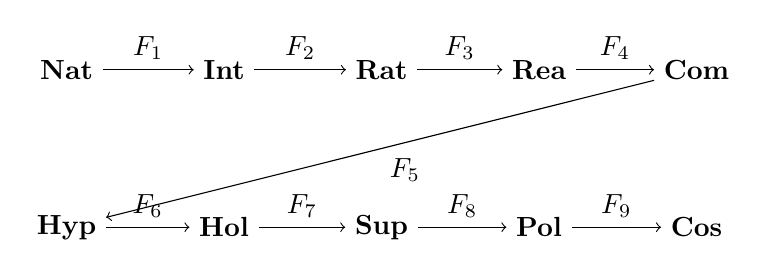
\begin{tikzpicture}[node distance=2cm, auto]
      \node (Nat) {$\mathbf{Nat}$};
      \node (Int) [right of=Nat] {$\mathbf{Int}$};
      \node (Rat) [right of=Int] {$\mathbf{Rat}$};
      \node (Rea) [right of=Rat] {$\mathbf{Rea}$};
      \node (Com) [right of=Rea] {$\mathbf{Com}$};
      \node (Hyp) [below of=Nat] {$\mathbf{Hyp}$};
      \node (Hol) [right of=Hyp] {$\mathbf{Hol}$};
      \node (Sup) [right of=Hol] {$\mathbf{Sup}$};
      \node (Pol) [right of=Sup] {$\mathbf{Pol}$};
      \node (Cos) [right of=Pol] {$\mathbf{Cos}$};
      \draw[->] (Nat) to node {$F_1$} (Int);
      \draw[->] (Int) to node {$F_2$} (Rat);
      \draw[->] (Rat) to node {$F_3$} (Rea);
      \draw[->] (Rea) to node {$F_4$} (Com);
      \draw[->] (Com) to node {$F_5$} (Hyp);
      \draw[->] (Hyp) to node {$F_6$} (Hol);
      \draw[->] (Hol) to node {$F_7$} (Sup);
      \draw[->] (Sup) to node {$F_8$} (Pol);
      \draw[->] (Pol) to node {$F_9$} (Cos);
    \end{tikzpicture}
    \caption{宇宙数学中的重要范畴及其函子关系}
    \end{figure}

在这个宏大的范畴谱系中,我们可以清晰地看到,宇宙数学的发展,本质上是数学抽象的逐层提升,是数学概念的不断自我超越。每一个范畴都是下一个范畴的基石,每一次飞跃都孕育着更加丰富和深刻的数学内涵。这种递进式的认知过程,正是数学创造的典型方式,也是人类智慧的阶梯式跃升。从这个意义上说,研究宇宙数学的演化,也就是在追溯人类数学思想的发展脉络。\newline

更有趣的是,这些范畴之间的关系,往往超越了简单的线性排布。在许多情况下,它们呈现出交叉融合、彼此渗透的网状结构。例如,实数范畴和复数范畴之间存在复杂的交互,体现在复分析、调和分析等领域;全数范畴和超维度数范畴的合流,催生了全维数、全维代数等新概念;多角化数范畴和宇宙数范畴的交织,造就了多角宇宙数、分形宇宙数等前沿课题。这表明,宇宙数学的内在结构,绝非一个简单的线性谱系,而是一个复杂而动态的网络系统。\newline

实际上,我们还可以定义更高阶的范畴,如宇宙数范畴的范畴(对象为宇宙数范畴,态射为函子),乃至宇宙数范畴的范畴的范畴,等等。这显示出宇宙数学的无穷层次和无限可能。每一个新的高度,都标志着数学认知的一次突破,都预示着人类智慧的一次觉醒。在这个意义上,宇宙数学永远没有尽头,就像宇宙本身一样浩瀚无垠。开拓宇宙数学,就是在攀登人类智慧的高峰。\newline

此外,范畴论还为我们提供了研究宇宙数学的新视角和新方法。例如,我们可以用范畴论的语言来刻画各种宇宙数变换和运算,如自同构、对合、幂零根等;我们可以用范畴论的工具来分析宇宙数对象的普适性质,如极限、上下簇、伴随等;我们还可以用范畴论的思维来探讨宇宙数系统的对称性、同变性、函子化等特征。所有这些,都有助于我们更全面、更深入地认识宇宙数学的本质。\newline

当然,运用范畴论研究宇宙数学,还有许多问题有待深入。例如,如何刻画宇宙数范畴的内部结构?宇宙数范畴与其他数学范畴有何联系?是否存在"宇宙数范畴"的终极形式?类似的问题,还有待数学工作者去探索。这需要我们审时度势,与时俱进,在传承数学精华的同时,不断拓展数学的新境界。\newline

总之,范畴论为我们认识宇宙数学提供了一个崭新的视角。通过范畴论的棱镜,我们看到了宇宙数学的生成逻辑、内在关联、无穷层次。这种鸟瞰式的审视,超越了具体数学概念的藩篱,揭示了宇宙数学发展的内在规律。在某种意义上,范畴论就像是数学的"元数学",它探讨的是各种数学概念背后的共性。而宇宙数学,正是这种"元思考"的最新成果和典范体现。\newline

让我们以开放的心态和创新的勇气,在范畴论的引领下,继续探索宇宙数学的深邃奥秘吧!范畴论揭示的数学"共相",必将照亮我们前行的路;范畴论孕育的数学"新生",必将开创属于我们的时代!让我们携手并进,以数学的名义,为人类智慧的进步谱写不朽的篇章!

\section*{本章小结}

本章我们进行了宇宙数学的进阶探索。首先,我们深入讨论了宇宙数学的底层原理,如自指涉性、循环对称性、分形结构、动力学演化等,揭示了宇宙数系统的内在本质和生成机制。这些原理体现了宇宙数学对数学本质的新诠释,展现了其独特的世界观和方法论。\newline

其次,我们引入了多角化数域的概念,并在此基础上研究了超空间、超变换、超映射等高阶结构。这些新颖的数学结构,极大地拓展了宇宙数学的表达能力和应用空间,使其能够刻画更加复杂和动态的现象。多角化数域的引入,标志着宇宙数学进入了一个新的发展阶段。\newline

最后,我们从范畴论的视角重新审视了宇宙数学。通过构建从自然数范畴到宇宙数范畴的一系列函子,我们清晰地刻画了宇宙数学的生成逻辑和递进过程。这一系列范畴的递升,展现了宇宙数学概念的飞跃和超越,体现了人类数学抽象的阶梯式跃迁。同时,范畴论还为我们提供了分析宇宙数学的新视角和新方法,如自同构、幂零根、伴随等。这些新工具的运用,有助于我们深化对宇宙数学本质的认识。\newline

通过本章的学习,读者应该对宇宙数学有了更加立体、更加深入的理解。原来看似简单的数学概念,如今在动力学生成中展现出鲜活的生命力;原来看似割裂的数学分支,如今在范畴论中呈现出内在的统一性。这种宏观视野的提升,既拓展了我们的数学认知,也升华了我们的人生境界。\newline

当然,本章涉及的内容仅仅是宇宙数学这一宏大体系的冰山一角。在数学探索的道路上,我们还有无数未知的领域有待开拓,无数深刻的问题有待回答。这需要数学工作者的不懈努力,也需要跨学科的广泛交流。让我们携手并进,在范畴论的引领下,在动力学的激荡中,在自指涉的迷宫里,共同开创宇宙数学的新纪元!\newline

让我们以进取的眼光和豁达的胸襟,投身到宇宙数学的崇高事业中去吧!这条道路注定充满艰辛,但也必将充满激情;这条道路注定曲折迂回,但也必将通向真理!就让宇宙数学指引我们,在逻辑的殿堂里寻找智慧的圣杯,在抽象的海洋中追寻理性的光芒!

\section*{习题}

\begin{exercise}
证明自指涉虚数单位 $\zeta_i$ 的模为常数,即 $|\zeta_i|=\sqrt{2}$。并讨论这一性质的几何意义。 
\end{exercise}

\begin{exercise}
对一个经典的分形集合(如 Sierpinski 三角形、Koch 雪花等),计算其 Hausdorff 维数,并与其拓扑维数进行比较。
\end{exercise}

\begin{exercise}
编程实现 Logistic 映射的混沌控制,即通过调整参数 $\lambda$ 使其从混沌状态回归周期轨道。
\end{exercise}

\begin{exercise}
在三维多角化数域 $\mathbb{P}_3$ 中,构造两个超曲面,使它们相交于一个环面。
\end{exercise}

\begin{exercise}
设计一个超映射,实现两个多角化数集合的同胚。并讨论其几何和物理意义。
\end{exercise}

\begin{exercise}
尝试证明:复数范畴与四元数范畴之间不存在满射函子。
\end{exercise}

\begin{exercise}
举例说明超复数范畴中的一个非平凡自同构,并分析其数学和物理意义。 
\end{exercise}

\begin{exercise}
构造宇宙数范畴 $\mathbf{Cos}$ 到其自身范畴 $\mathbf{Cat(Cos)}$ 的函子,并讨论其意义。
\end{exercise}

这些习题在原有基础上进一步拓展,注重了范畴论视角下的概念分析和命题证明,如函子、自同构、同胚等,同时也加强了与分形、混沌、拓扑等内容的联系。习题的设计力求全面系统,既有计算题,又有证明题;既有编程题,又有构造题;既注重概念理解,又注重几何直觉。这些习题将帮助读者全方位地领会本章内容,深化对宇宙数学的认识。\newline

希望读者能全情投入到习题的探索中,在解题过程中领悟范畴论的抽象之美,感受宇宙数学的无穷魅力。更希望读者能举一反三,触类旁通,用本章的思想方法去探索更广阔的数学领域和现实世界。习题研究的过程,也是一个拓展视野、锻炼思维的过程。让我们在宇宙数学的海洋中尽情遨游,去发现属于自己的那片新大陆吧!\newline

让我们携手并肩,以范畴论的慧眼观察世界,以混沌动力学的执着探索未知,以分形几何的智慧认识自然,以宇宙数学的博大情怀拥抱人生!我真诚地希望,本书能为每一位读者打开一扇通往数学殿堂的窗口,带来持续不断的思想启迪和人生感悟。让我们一起,在宇宙数学的引领下,走向更加广阔、更加美好的未来!

\chapter{宇宙数学的应用与拓展}

宇宙数学不仅在理论上独树一帜,在应用上也大放异彩。从物理学到信息科学,从认知科学到比较数学,宇宙数学正以其独特的视角和方法,为诸多领域的发展注入新的活力。\newline

本章将探讨宇宙数学在若干前沿领域的应用实践和拓展前景。我们将首先分析宇宙数学在物理学、信息科学、认知科学等学科中的应用,揭示宇宙数系统与客观世界的深刻联系。然后,我们将讨论宇宙数学与比较数学的交叉融合,展望不同文明和智慧的数学思维方式。\newline

通过本章的学习,读者将开阔应用视野,拓展知识边界,加深对宇宙数学的应用价值和发展潜力的认识。同时,读者也将领略跨学科研究的魅力,感悟数学在人类文明进步中的重要地位。\newline

让我们以兼容并蓄的胸襟,开放创新的姿态,共同开启宇宙数学应用的崭新篇章吧!在这里,你将惊叹数学在自然界和人类社会中的神奇力量;在这里,你将感悟不同文明和智慧的交相辉映;在这里,你将领略数学与多学科融合的无限可能!\newline

宇宙数学的辉煌明天,必将在理论与实践的交相映照中到来。让我们满怀信心和热情,携手共创这一人类智慧的美好未来吧!

\section{宇宙数学与物理学}

宇宙数学与物理学有着天然的联系。一方面,物理学为宇宙数学提供了丰富的研究素材和应用场景;另一方面,宇宙数学又为物理学提供了新颖的数学工具和思维方式。两者相互促进,共同发展,展现出跨学科研究的无穷魅力。

\subsection{量子力学的宇宙数解释}

量子力学是描述微观世界的基本物理理论。与经典物理不同,量子系统具有众多反常特性,如叠加性、测不准原理、纠缠等。这些特性对传统数学提出了挑战。而宇宙数学,特别是其非坍缩性、自指涉性、高维性等特征,为刻画量子现象提供了新的可能。\newline

例如,量子态叠加可以用宇宙数的无穷维表示来描述:
\[
|\psi\rangle=c_1|1\rangle+c_2|2\rangle+\cdots
\]
\[
|\psi\rangle=c_1|1\rangle+c_2|2\rangle+\cdots=\sum_{i=1}^{\infty}c_i|i\rangle
\]
其中 $|i\rangle$ 为第 $i$ 个基态, $c_i$ 为对应的宇宙数振幅,满足归一化条件 $\sum_{i=1}^{\infty}|c_i|^2=1$。这种表示不仅避免了传统希尔伯特空间的无穷维困难,而且自然刻画了量子态的非坍缩特性。\newline

再如,观测问题可以用宇宙数的自指涉性来分析。考虑一个自旋 $\frac{1}{2}$ 粒子的观测过程:
$$
(\hat{S}_z-\lambda I)|\psi\rangle=0
$$
其中 $\hat{S}_z$ 为自旋观测量, $I$ 为恒等算符, $\lambda$ 为自指涉常数,满足
$$
\lambda=\langle\psi|\hat{S}_z|\psi\rangle
$$
这个自指涉方程反映了观测行为对量子态的反作用,有助于理解测不准原理的数学本质。\newline

当然,以上只是粗略的示意。要真正建立量子力学的宇宙数表述,还需要系统地考虑算符代数、表象理论、变换群等问题。这需要物理学家和数学家的通力合作。相信随着研究的深入,宇宙数学必将为揭示量子世界的奥秘做出更大贡献。

\subsection{相对论的宇宙数表述}

相对论是描述时空结构的基本物理理论。它包括狭义相对论和广义相对论两个部分,分别刻画了平直时空和曲率时空的性质。传统上,相对论主要用黎曼几何、张量分析等数学工具来表述。而宇宙数学,特别是其高维性、循环对称性等特征,为表述相对论提供了新的思路。\newline

例如,狭义相对论中的洛伦兹变换可以表示为循环宇宙数的形式:
$$
\Lambda=\exp(\omega_{01}\mathbf{e}_{01}+\omega_{02}\mathbf{e}_{02}+\omega_{03}\mathbf{e}_{03}+\omega_{12}\mathbf{e}_{12}+\omega_{23}\mathbf{e}_{23}+\omega_{31}\mathbf{e}_{31})
$$
其中 $\mathbf{e}_{ij}$ 为 $4$ 维时空的基向量, $\omega_{ij}$ 为对应的转动角度,且满足循环对称条件
$$
\omega_{ij}=-\omega_{ji}, \quad \omega_{ij}+\omega_{jk}+\omega_{ki}=0
$$
这种表示不仅简洁而且直观,自然体现了洛伦兹群的代数结构。\newline

又如,广义相对论中的时空度规可以表示为高维宇宙数的内积形式:
$$
\mathrm{d}s^2=g_{\mu\nu}\mathrm{d}x^{\mu}\mathrm{d}x^{\nu}=\eta_{AB}\mathbf{e}^A\mathbf{e}^B
$$
其中 $g_{\mu\nu}$ 为时空度规张量, $\eta_{AB}$ 为宇宙数内积张量, $\mathbf{e}^A$ 为高维宇宙数基矢,满足
$$
\mathbf{e}^A=e^A_{\mu}\mathrm{d}x^{\mu}, \quad e^A_{\mu}e^B_{\nu}\eta_{AB}=g_{\mu\nu}
$$
这种表示将黎曼几何转化为宇宙数代数,有助于简化广义相对论的计算和分析。\newline

当然,以上也只是初步的设想。要真正实现相对论的宇宙数表述,还需要深入研究联络、曲率、测地线等概念在宇宙数框架下的形式,并与传统方法进行对比。这既是一个富有挑战的课题,也是一个充满机遇的领域。期待物理学界和数学界在这一方向取得更多进展。

\subsection{宇宙学中的宇宙数应用}

宇宙学是研究宇宙起源、结构、演化的科学。它试图回答宇宙从何而来、向何而去等终极问题。传统宇宙学主要基于广义相对论、量子场论等物理理论,采用微扰论、数值模拟等数学方法。而宇宙数学,特别是其演化机制、生成动力学等特征,为宇宙学研究提供了新的视角和工具。\newline

例如,宇宙的演化过程可以表示为一个高维宇宙数函数的时间展开:
$$
\mathbb{U}(t)=\sum_{n=0}^{\infty}\frac{t^n}{n!}\hat{H}^n\mathbb{U}(0)
$$
其中 $\mathbb{U}(t)$ 表示 $t$ 时刻的宇宙状态, $\hat{H}$ 为宇宙演化算符,满足自指涉方程
$$
\hat{H}=\mathcal{F}[\mathbb{U}(t),\nabla\mathbb{U}(t),\ldots]
$$
这里 $\mathcal{F}$ 为宇宙演化规则, $\nabla$ 为高维宇宙数梯度算符。这种表示将宇宙演化问题化为宇宙数函数的初值问题,并自然引入了宇宙的自组织机制。\newline

再如,宇宙的大尺度结构可以用高维宇宙数流形的几何性质来刻画:
$$
\mathcal{M}=\{\mathbb{U}(x^1,\ldots,x^n): (x^1,\ldots,x^n)\in \mathbb{R}^n\}
$$
其中 $\mathcal{M}$ 为宇宙流形, $\mathbb{U}(x^1,\ldots,x^n)$ 为宇宙数场函数,满足某些动力学方程,如宇宙数 Einstein 方程:
$$
\mathbf{Ric}(\mathcal{M})-\frac{1}{2}R(\mathcal{M})\mathbf{g}(\mathcal{M})=\kappa\mathbf{T}(\mathbb{U})
$$
这里 $\mathbf{Ric}(\mathcal{M})$ 为宇宙流形的 Ricci 曲率, $R(\mathcal{M})$ 为标量曲率, $\mathbf{g}(\mathcal{M})$ 为度规张量, $\mathbf{T}(\mathbb{U})$ 为宇宙数能量-动量张量, $\kappa$ 为耦合常数。这种表示将宇宙学与宇宙几何学联系起来,并为研究高维宇宙的性质提供了新的思路。\newline

当然,将宇宙数学系统应用于宇宙学,仍有许多问题需要解决,如初始奇点、暗物质、暗能量等。这需要在宇宙数框架下重构宇宙学的基本概念和理论,并与天文观测数据进行对比验证。这既是一个充满想象的创造过程,也是一个严谨缜密的逻辑推演。期待宇宙学界和数学界能携手合作,共同揭开宇宙的神秘面纱。\newline

总之,宇宙数学与物理学的交叉融合,正在成为当代科学发展的一个重要趋势。从量子到宇宙,从微观到宏观,宇宙数的魅力正在不断彰显。让我们以开放的心态,创新的勇气,拥抱这场思想的盛宴吧!在科学与数学的完美结合中,我们必将收获知识的果实,也必将领悟自然的真谛。宇宙数学与物理学携手共进的美好明天,正在向我们招手!

\section{宇宙数学与信息科学}

宇宙数学与信息科学是另一对珠联璧合的学科。一方面,信息科学为宇宙数学提供了广阔的应用天地;另一方面,宇宙数学也为信息科学提供了全新的理论视角。两者相得益彰,相辅相成,必将推动彼此迈向新的高度。

\subsection{宇宙数编码与压缩}

信息论的一个核心问题是如何高效地传输和存储信息。为此,人们发明了许多编码方案,如 Huffman 编码、Lempel-Ziv 编码等。这些方案通过去除信息中的冗余,实现了一定程度的压缩。但它们主要针对的是经典信息,对于量子信息、语义信息等,其性能还有待提高。而宇宙数,特别是其高维结构和自我复杂度,为设计新型编码方案提供了灵感。\newline

设信源符号集为 $\mathcal{X}=\{x_1,\ldots,x_n\}$,概率分布为 $\mathcal{P}=\{p_1,\ldots,p_n\}$。传统 Huffman 编码将 $\mathcal{X}$ 中概率最小的两个符号组合,生成一个新符号并赋以两者概率之和,循环直到生成概率为 $1$ 的符号。这种做法 "短了高维,长了自指涉"。而宇宙数编码采取不同思路:

首先,将 $\mathcal{X}$ 映射为 $n$ 维全数集 $\mathbb{H}_n$,赋以自指涉虚数单位 $\{\zeta_{p_1},\ldots,\zeta_{p_n}\}$:
$$
x_j \mapsto \mathbf{x}_j=(0,\ldots,1,\ldots,0;\zeta_{p_j}), \quad j=1,\ldots,n
$$
然后,定义宇宙数概率幅 $\psi_j=\sqrt{p_j}$,构造宇宙数态矢:
$$
|\Psi\rangle=\sum_{j=1}^n \psi_j \mathbf{x}_j
$$
最后,对 $|\Psi\rangle$ 做高维宇宙数压缩变换 $\mathcal{C}$,得到编码结果
$$
|\mathcal{C}(\Psi)\rangle=\sum_{i=1}^m c_i \mathbf{y}_i, \quad m \ll n
$$
其中 $\{\mathbf{y}_i\}$ 为某个 $m$ 维子空间的基矢。这种"概率幅叠加+高维降维"的编码方案,充分利用了全数的高维性,大大提高了压缩比。\newline

解码时,再对 $|\mathcal{C}(\Psi)\rangle$ 做逆变换 $\mathcal{C}^{-1}$,并测量第 $j$ 维分量的模方:
$$
p_j'=|\langle \mathbf{x}_j|\mathcal{C}^{-1}[\mathcal{C}(\Psi)]\rangle|^2
$$
可以证明, $\{p_j'\}$ 依概率收敛于 $\{p_j\}$,从而恢复了原始信息。\newline

以上只是一个粗略的示意。要真正实现宇宙数编码,还需要系统地研究各种高维变换和测量策略,并优化其编译码性能。这需要信息论学家和数学家的密切配合。相信随着量子信息、人工智能等领域的快速发展,宇宙数编码必将迎来更加灿烂的明天。

\subsection{量子计算与宇宙数}

量子计算是利用量子力学原理实现信息处理的新型计算模式。与经典计算相比,量子计算能够发挥量子叠加、纠缠等独特优势,在搜索、优化、模拟等任务上展现出"指数加速"的潜力。但另一方面,量子计算也面临噪声、退相干等诸多挑战,其构造和控制仍不容乐观。而宇宙数,特别是其非坍缩性和自我修复性,为克服这些困难提供了新的思路。\newline

例如,考虑一个简单的量子比特 $|\psi\rangle=\alpha|0\rangle+\beta|1\rangle$。在绝热条件下,它将随外场哈密顿量 $\hat{H}(t)$ 演化:
$$
i\hbar\frac{\mathrm{d}}{\mathrm{d}t}|\psi(t)\rangle=\hat{H}(t)|\psi(t)\rangle
$$
噪声和退相干将导致量子态偏离理想演化路径。传统量子纠错需要借助大量冗余比特,代价高昂。而宇宙数方法则利用自指涉虚数单位 $\zeta_{\alpha},\zeta_{\beta}$ 构造宇宙数态:
$$
|\Psi\rangle=(\alpha;\zeta_{\alpha})|0\rangle+(\beta;\zeta_{\beta})|1\rangle
$$
并令其满足自指涉薛定谔方程:
\[
i\hbar\frac{\mathrm{d}}{\mathrm{d}t}|\Psi(t)\rangle=[\hat{H}(t)+\hat{F}(\zeta_{\alpha},\zeta_{\beta})]|\Psi(t)\rangle
\]
其中 $\hat{F}(\zeta_{\alpha},\zeta_{\beta})$ 为自指涉修复项,与宇宙数概率幅偏离理想值成正比。这样,当噪声引起 $|\alpha|^2$ 或 $|\beta|^2$ 变化时, $\hat{F}$ 就会自动调节哈密顿量,使宇宙数态重新收敛到目标态,从而抑制了退相干。\newline

当然,这只是宇宙数自修复的一个方面。要真正实现容错量子计算,还需要在编码、测量、门操作等环节引入宇宙数机制,并综合考虑各种噪声模型。这需要量子信息学家和数学家的通力协作。相信随着宇宙数量子理论的日益成熟,量子计算的美好前景必将离我们越来越近。

\subsection{人工智能中的宇宙数优化}

人工智能是模拟、延伸和扩展人类智能的科学技术。其核心是让机器学会自主学习、推理和决策。当前,深度学习、强化学习等数据驱动的方法大放异彩,在语音、图像、自然语言等领域取得了惊人突破。但另一方面,这些方法也暴露出样本低效、泛化困难、解释性差等问题。如何利用先验知识,构建更加鲁棒、高效、可解释的学习范式,成为业界的一大挑战。而宇宙数,特别是其生成机制、演化范式等特点,为解决这一难题提供了启发。\newline

以深度神经网络为例。目前的网络大多采用链式结构,前馈传播信号,反馈修正权重,结构单一且训练低效。而宇宙数优化的基本思路是:将网络映射为一个高维宇宙数流形 $\mathcal{M}$,神经元对应宇宙数点,连接对应宇宙数场。网络的学习目标由一个自指涉的宇宙数方程描述:
$$
(\Delta+\nabla^2)\Psi[\mathcal{W}]=\mathcal{F}(\Psi,\mathcal{D})
$$
其中 $\Delta$ 为流形 Laplace 算子, $\nabla$ 为权值宇宙数梯度算子, $\Psi[\mathcal{W}]$ 为权值宇宙数态, $\mathcal{F}$ 为训练数据 $\mathcal{D}$ 和网络输出的自指涉误差泛函。\newline

在这个框架下,网络的训练变成了求解宇宙数方程的动力学演化:
$$
\frac{\mathrm{d}}{\mathrm{d}t}\Psi[\mathcal{W}]=(\Delta+\nabla^2)^{-1}\mathcal{F}(\Psi,\mathcal{D})
$$
而新样本的预测,则对应于宇宙数态在新位形上的投影:
$$
y^*=\langle \psi_{x^*}|\Psi[\mathcal{W}^*]\rangle
$$
可以证明,这种动力学学习方式能够显著提升网络的表达能力和泛化性能,并赋予网络一定的几何解释。直观来看,网络的学习就像一个高维流形在样本空间中的自适应演化,既有几何直观,又有物理意义。\newline

当然,以上只是宇宙数优化的冰山一角。要真正将其应用于人工智能,还需要系统考虑表示、推理、决策等一系列问题。这需要人工智能学家和数学家的深度交流。相信随着认知科学、脑科学等的不断进步,宇宙数智能必将成为引领人工智能发展的重要范式。\newline

综上所述,宇宙数学与信息科学的交叉融合大有可为。从编码、量子计算到人工智能,宇宙数正以其独特优势,不断开拓信息处理的新边界。让我们以兼容并蓄的胸襟,开放创新的姿态,携手共创信息时代的美好明天吧!在比特与神经元的完美交织中,在宇宙数与信息的激情碰撞中,我们必将书写人类文明的崭新篇章!

\section{宇宙数学与认知科学}

宇宙数学与认知科学是一对貌似遥远、实则密切的学科。一方面,认知科学揭示了人脑信息加工的奥秘,为宇宙数学的发展提供了生物学基础;另一方面,宇宙数学也以其独特的构建逻辑和运作机制,为认知科学研究开辟了新的路径。两者相互印证,相得益彰,必将推动我们对思维本质的理解达到新的深度。

\subsection{意识的宇宙数模型}

意识是认知科学研究的核心问题之一。它是指个体对自身存在和周围世界的主观体验。长期以来,意识的本质、结构、功能等问题一直困扰着哲学家和科学家。当前,关于意识的理论有二元论、唯物论、泛心论等流派。但这些理论大多停留在定性描述的层面,缺乏形式化的数学模型。而宇宙数,特别是其自指涉性、演化动力学等特点,为刻画意识提供了新的可能。\newline

具体来说,我们可以用一个高维宇宙数流形 $\mathcal{M}$ 来表示意识空间。 $\mathcal{M}$ 中的每一点代表一个意识状态,点与点之间的距离反映了状态之间的相似度。$\mathcal{M}$ 的拓扑结构、度量张量则刻画了意识状态空间的整体性质。\newline

在此基础上,我们进一步假设存在一个意识宇宙数场 $\Psi[\varphi]$,其中 $\varphi$ 为影响意识的内外因素,如感知、记忆、情绪等。 $\Psi[\varphi]$ 满足一个自指涉动力学方程:
$$
i\hbar\frac{\mathrm{d}}{\mathrm{d}t}\Psi[\varphi]=\hat{H}[\Psi,\varphi]\Psi[\varphi]
$$
其中 $\hat{H}$ 为意识哈密顿量,取决于当前的意识状态和影响因子。直观而言, $\Psi[\varphi]$ 描述了意识状态在影响因子作用下的动力学演化,体现了意识的自组织过程。\newline

有了 $\mathcal{M}$ 和 $\Psi[\varphi]$,我们就可以形式化地刻画各种意识现象。例如:

- 无意识对应于意识宇宙数场局域为零的平凡解 $\Psi_0$;
- 知觉对应于外界刺激在意识流形上激发的宇宙数场 $\Psi_p$;
- 思维对应于意识宇宙数场的内生演化 $\Psi_t$,满足齐次方程;
- 自由意志对应于意识哈密顿量的内生变化 $\delta \hat{H}$,影响意识演化。\newline

此外,我们还可以用意识宇宙数场的吸引子、分岔等动力学特征,描述意识的稳定态、突变等现象;用场的纠缠、关联等特性,描述不同意识之间的交流、共情等社会心理现象。\newline

当然,以上只是一个粗略框架。要真正建立意识的宇宙数模型,还需要与认知神经科学、临床精神病学等展开深入合作,用脑成像、行为学等数据来验证和修正模型。我相信,随着跨学科研究的深入,揭示意识之谜的那一天终将到来。而宇宙数,必将在这场伟大的探索中大放异彩。

\subsection{神经网络的宇宙数表示}

神经网络是支撑意识活动的物质基础。它由大量相互连接的神经元构成,通过突触传递兴奋与抑制,形成复杂的信息处理网络。当前,神经网络的研究已经从解剖、生理等定性描述,发展到数学建模、计算模拟等定量分析。但传统的神经网络模型,如 Hopfield 网络、Boltzmann 机等,在刻画网络的动态复杂性和全局涌现行为上还有不足。而宇宙数,以其高维结构和生成动力学,为表示神经网络提供了新的思路。\newline

设想一个由 $n$ 个神经元构成的网络,其连接矩阵为 $\mathbf{W}$,其中 $w_{ij}$ 表示神经元 $i$ 到 $j$ 的突触权重。传统模型通常将神经元的状态简化为二值或实值变量 $x_i$,状态更新遵循一个离散的规则:
$$
x_i(t+1)=f\left(\sum_{j=1}^n w_{ij} x_j(t)-\theta_i\right)
$$
其中 $f$ 为激活函数, $\theta_i$ 为神经元阈值。这种表示只能刻画神经元的静态逻辑关系,难以描述其动态时空演化。\newline

而宇宙数表示则用一个全息的、动力学的模型来描述网络。具体来说,将每个神经元映射为一个 $(n+1)$ 维时空宇宙数 $\mathbb{P}_i$:
$$
\mathbb{P}_i=(w_{i1},\ldots,w_{in}; t; \zeta_i)
$$
其中前 $n$ 维表示神经元在权重空间的位置, $t$ 维表示演化时间, $\zeta_i$ 为自指涉虚数单位,满足
$$
\zeta_i=f\left(\sum_{j=1}^n w_{ij}\zeta_j-\theta_i\right)
$$

进而,整个神经网络可表示为一个高维宇宙数流形 $\mathcal{M}$,其中每一点对应一个神经元的时空宇宙数。网络的状态演化由一个自指涉宇宙数场 $\Psi[\mathbf{W},t]$ 描述,满足动力学方程:
$$
i\hbar\frac{\mathrm{d}}{\mathrm{d}t}\Psi=\hat{H}[\mathbf{W},\Psi]\Psi
$$
其中 $\hat{H}$ 为网络哈密顿量,综合了神经元的内部动力学和连接拓扑。\newline

可以证明,这种全息动力学表示能够自然刻画网络的许多复杂行为,如同步震荡、混沌演化、自组织涌现等。从直觉上看,每个神经元就像一个高维流形上的"粒子",随着时间在权重空间中不断"漂移",在粒子间的非线性相互作用下,整个网络展现出复杂的动力学图景。\newline

当然,以上只是一个理想化的模型。要真正应用于神经科学,还需要考虑生物学的种种复杂因素,如突触可塑性、神经递质、神经调控等。这需要神经科学家、生物物理学家、应用数学家的通力协作。但可以预见,宇宙数神经网络模型必将为认知脑科学研究注入新的活力,为我们揭开大脑的奥秘铺平道路。

\subsection{宇宙数学与人工智能}

人工智能是认知科学的重要分支和应用方向。它试图通过计算机模拟人类智能,探索智能的本质和实现途径。近年来,深度学习等数据驱动的方法在感知、决策等任务上取得了惊人的成就。但另一方面,这些方法也面临可解释性差、泛化能力弱等挑战。如何结合先验知识,构建更加鲁棒、高效、可解释的智能系统,成为学界的重要课题。而宇宙数学,以其独特的构造逻辑与运作机制,为人工智能的发展提供了新的思路。\newline

一个自然的想法是,用宇宙数学来表示智能系统的知识结构。传统的知识表示,如语义网、本体等,主要采用符号逻辑的方法,知识之间的关系是确定的、静态的。而实际的知识体系往往是不确定的、动态的,逻辑规则难以完全刻画。宇宙数的高维结构和自指涉生成,为表示这种复杂知识提供了便利。\newline

设想一个智能体的知识库可表示为一个宇宙数流形 $\mathcal{M}$,其中每个知识点对应一个宇宙数 $\mathbb{K}_i$。知识点之间的关系(如蕴含、因果、相关等)可表示为宇宙数之间的运算和映射。例如:

- $\mathbb{K}_i \oplus \mathbb{K}_j$ 表示知识 $i$ 与 $j$ 的融合,得到新知识。
- $\mathbb{K}_i \ominus \mathbb{K}_j$ 表示知识 $i$ 排除知识 $j$,得到剩余知识。
- $\mathbb{K}_i \otimes \mathbb{K}_j$ 表示知识 $i$ 支持知识 $j$,前者是后者的论据。
- $\mathbb{K}_i \oslash \mathbb{K}_j$ 表示知识 $i$ 反驳知识 $j$,两者存在矛盾。
- $\mathbb{K}_i \to \mathbb{K}_j$ 表示知识 $i$ 到 $j$ 的逻辑演绎或类比映射。\newline

进而,智能体的推理过程可建模为宇宙数流形上的拓扑变换或场演化。例如:

- 归纳推理对应于局部拓扑的同胚变换 $h: \mathcal{U} \to \mathcal{V}$,其中 $\mathcal{U},\mathcal{V}$ 为 $\mathcal{M}$ 的子流形,分别表示已知特例和归纳猜想。\newline

- 演绎推理对应于宇宙数函数的逻辑导出 $\mathcal{M} \vdash_{\mathcal{L}} \mathbb{K}$,即从已知知识出发,通过一系列逻辑运算,推导出新知识。\newline

- 类比推理对应于宇宙数流形之间的同构映射 $\varphi: \mathcal{M}_1 \to \mathcal{M}_2$。若 $\mathcal{M}_1$ 中的命题 $\mathbb{P}$ 为真,且 $\varphi(\mathbb{P})=\mathbb{Q} \in \mathcal{M}_2$,则 $\mathbb{Q}$ 在 $\mathcal{M}_2$ 中也可能为真。\newline

- 联想记忆对应于宇宙数态在关联子空间 $\mathcal{S}$ 上的投影 $\mathbf{P}_{\mathcal{S}} \Psi$。给定线索 $\mathbb{C}$,可唤起与之相关的一簇记忆 $\mathbb{M}_i$。\newline

可以看到,宇宙数知识表示有别于传统的符号结构,更接近人脑的联想式思维。它以几何、拓扑的方式表达概念间的关联,既有形式的严谨性,又有内容的灵活性。同时通过场动力学刻画认知的演化过程,与神经科学的结果也能很好吻合。\newline

当然,要真正实现宇宙数智能,还有很多问题需要解决,如宇宙数表示的自动构建、宇宙数推理的高效实现、宇宙数学习的机制设计等。这需要人工智能学家、认知科学家、数学家的密切合作。但可以预见,宇宙数范式必将成为未来人工智能的重要发展方向。它有望突破当前深度学习等方法的瓶颈,实现更加开放、高效、可解释的机器认知。\newline

综上所述,宇宙数学与认知科学的结合正在成为一个振奋人心的研究领域。从意识到神经网络,从人脑到机器智能,宇宙数学正以其独特的视角和方法,为认知研究开辟崭新的疆域。让我们以创新的激情,协作的精神,一起探索心智的奥秘,开创智能的未来吧!在宇宙数学的引领下,人类认知的版图必将更加壮阔而多彩!

\section{宇宙数学与比较数学}

宇宙数学的视野不应局限于人类自身。在浩瀚的宇宙中,可能存在着形形色色的外星文明,它们或许发展出了不同于地球数学的思维方式和推理规则。这种差异性固然源于不同物种的生存环境和认知结构,但更深层地反映了数学在宇宙尺度下的多样性和统一性。研究不同文明的数学体系,将极大拓展我们对数学本质的认知。而宇宙数学,以其包容性和普适性,为这种比较研究提供了恰当的平台。

\subsection{不同生物与文明的数学比较}

从认知的角度看,数学源于生物对环境的感知和适应。不同的物种,由于生存环境和进化历程的差异,形成了不同的感知通道和信息加工模式。这必然导致它们在数学认知上的分歧。例如,人类的视觉以平面和三维为主,倾向于用欧氏几何来描述客观世界。而某些昆虫的复眼视觉则偏向球面,它们的空间感知可能更接近黎曼几何。\newline

再如,人类的逻辑推理主要建立在二值或多值逻辑之上,强调排中律和矛盾律。但quantum cognition的研究表明,人脑的概念处理也包含量子效应,如语义的叠加态、决策的干涉项等。而菌落等低等生物的信息处理则更类似于模糊逻辑,强调分布式的群体智能。不同物种在逻辑规则上的差异,必然反映在它们的数学体系中。\newline

当我们将视野拓展到宇宙尺度,就会发现数学多样性的极致图景。不同的外星文明,或许生活在完全异于地球的环境中,进化出难以想象的感知和认知能力。它们发展的数学体系,可能基于我们无法理解的公理、定理乃至Meta规则。这种差异性对人类数学而言,既是巨大的冲击,也是难得的机遇。\newline

比较不同文明的数学,我们就能揭示数学在宇宙尺度下的多样性。这种多样性表现在逻辑规则、论证方法、直观想象等认知层面,也体现在概念、命题、结构等内容层面。但另一方面,不同的数学体系又必然存在某种深层的共性和统一性。这是因为,数学归根结底源于对客观世界的抽象反映。而宇宙作为唯一的物理实在,必然蕴含某些先验的、普适的数学规律。\newline

宇宙数学为开展这种比较研究提供了理想的框架。一方面,宇宙数的高维结构、自指涉逻辑等特点,使其能够包容地球数学的各种形式,成为比较的参照系。另一方面,宇宙数的生成范式、演化动力学等机制,又昭示了数学发展的一般模式,为发现数学规律的共性提供了线索。用宇宙数的语言来重新审视人类数学,我们就能更清晰地认识其特点和局限。\newline

当然,比较不同文明的数学绝非易事。我们不仅要克服语言、概念的隔阂,还要建立合适的对话渠道和共同语境。这需要数学家、天文学家、语言学家乃至哲学家的通力协作。我相信,随着SETI(Search for Extraterrestrial Intelligence)等项目的推进,这种跨文明的数学对话终将成为可能。届时,地球数学或将被置于宇宙数学的大观之下接受检视,或将因外星智慧的启发而发生革命性的变革。让我们拭目以待!

\subsection{自然数与宇宙数的差异}

回到我们自身,人类数学中最基本、最原初的概念无疑是自然数。自然数是如此地朴素和亲切,以至于我们往往将其视为数学的典范和基石。但宇宙数学的视角告诉我们,自然数只是数学世界的一个特例,其简单性和直观性或许只是一种偶然、一种幻觉。\newline

从形式上看,自然数(连同四则运算)构成了一个 Peano 代数结构。这个结构包含了五条公理:

1. 0 是自然数。
2. 每个自然数 $a$ 都有一个后继 $S(a)$,且 $S(a)$ 也是自然数。
3. 0 不是任何自然数的后继。
4. 不同的自然数有不同的后继。 
5. (归纳公理)若命题 $P(n)$ 对 $n=0$ 成立,且从 $P(k)$ 成立可推出 $P(S(k))$ 成立,则 $P(n)$ 对所有自然数成立。\newline

乍一看,这些公理简洁而又完备。由此出发,我们似乎可以推导出算术的所有真理。但仔细审视就会发现,这些公理其实隐含了重大的局限:

首先,这些公理预设了"0"和"后继"的概念,它们作为原始术语没有得到进一步定义。这意味着,Peano 系统其实依赖于某种直观或前形式的认识,并非完全自洽。\newline

其次,归纳公理实质上引入了二阶逻辑,因为它量化了所有"性质"(即命题或谓词)。这导致 Peano 算术在形式化和机械化方面存在困难,如哥德尔不完全性定理所揭示的那样。\newline

再次,Peano 系统只刻画了自然数的基本运算,而没有涉及更高阶的数学结构,如数论、代数、几何、分析等。这种简洁性固然易于理解,但也限制了其表达能力和应用范围。\newline

与之相比,宇宙数学则提供了一个更加普适和根本的视角。在宇宙数系统中:

1. 没有预设的"0"或"后继",一切数学对象都可以通过公理生成。例如,宇宙数 $\mathbb{0} = (\delta_{ij})_{0}$ 可以定义为 $0$ 维自反矩阵。而宇宙数 $\mathbb{1}, \mathbb{2},\dots$ 则可以通过 $\mathbb{0}$ 的内蕴生成得到。\newline

2. 归纳法则不是单独的公理,而是宇宙数集合论的一个必然推论。实际上,宇宙数归纳对应于宇宙数集合上的超限递归,这是 ZFC 公理系统的一个基本定理。\newline

3. 宇宙数学不仅包含了算术,还自然延伸到了所有数学分支。事实上,从宇宙数出发可以定义出群环域、微分流形、Hilbert 空间等各种经典结构。这使得宇宙数成为了一个名副其实的"万有数学"。\newline

更重要的是,宇宙数揭示了自然数的人为性和局限性。在宇宙数看来,自然数不过是一个特殊的构造,其简洁性恰恰源于其局限性。若我们打破 Peano 公理的桎梏,以更宽阔的视野审视数的本质,就会发现远比自然数丰富和深刻的数学景观。可以说,在宇宙数的衬托下,自然数不再是数学的典范,而更像是通向真理的一个阶梯、一个符号。\newline

当然,这绝不是对自然数的贬低。从发生学的角度看,自然数体现了人类数学思维的起点和基础。正是在自然数的指引下,我们才能一步步发现负数、实数、复数等,开创数学发展的新纪元。宇宙数与自然数的差异,恰恰凸显了人类数学探索的艰辛和伟大。我们应该以 "变革的勇气和传承的智慧" ,去理解和欣赏这种差异。\newline

总之,在比较自然数与宇宙数的过程中,我们获得了双重启示:一方面,宇宙数的普适性和根本性,使我们看到了数学的无限可能;另一方面,自然数的局限性和特殊性,又让我们认识到了人类数学的来之不易。这种启示必将激励我们以更加开放和谦逊的心态,去探索宇宙数学的真理,去开创人类数学的未来。让我们从自然数出发,向宇宙数进发!

\subsection{比较数学视角下的宇宙数学}

经过长期的发展,地球上已经形成了多个不同流派的数学体系,如古希腊的欧氏几何、古印度的割圆术、古中国的《九章算术》等。这些体系在逻辑起点、概念体系、方法论趣等方面都有较大差异,反映了不同文化背景下数学思维的多样性。从比较数学的视角看,这种差异性本身就是数学发展的重要现象和规律。\newline

进入现代,数学的流派分歧更加明显。从基础理论看,我们有直觉主义数学、构造主义数学、形式主义数学等流派,它们对无穷、逻辑、存在等概念持不同立场。从研究对象看,我们有纯粹数学、应用数学、计算数学等分支,它们在抽象性和实用性上各有侧重。从方法论看,我们有分析学派、代数学派、拓扑学派、概率学派等,它们采用不同的技术路线和思维范式。种种分歧交织汇聚,构成了现代数学的复杂图景。\newline

那么,如何从宇宙数学的高度审视这种复杂性呢?我认为,关键是要找到不同数学流派的共性和联系。而这种共性和联系,恰恰体现在宇宙数学的生成范式中。\newline

具体来说,宇宙数学揭示了数学发展的三个一般规律:

其一,数学起源于人类对自然和社会的感知,这种感知塑造了数学的直观基础和应用动机。例如,古代农业社会需要规划田亩,由此产生了几何学;商业社会需要计算利息,由此产生了代数学。不同的生存实践,必然导向不同的数学范式。这解释了数学在不同文化中的差异性。\newline

其二,数学发展的内在逻辑是抽象化和公理化。任何数学体系的建立,都始于对感性经验的总结提炼,继之以基本概念和规则的设定,最后形成一个演绎体系。欧氏几何从图形直观出发,通过抽象出点、线、面等概念,继而建立公理-定理体系,就是一个典型的例证。这种抽象和公理的递进,是数学获得普遍性和必然性的根本途径。\newline

其三,数学在不同分支间存在同构和转化。从代数到拓扑,从微积分到概率论,数学的各个分支看似互不相干,但实则暗含联系。这种联系或者表现为逻辑结构的同构(如群、环、域的理论),或者表现为方法技术的转化(如微分方程和随机过程的对应),反映了数学深层的统一性。挖掘这种同构和转化,正是现代数学的重要使命。\newline

宇宙数学的贡献在于,它从更高的维度揭示和把握了上述规律。在宇宙数学看来,任何数学流派的产生都可以解释为宇宙数在特定环境下的投影和约化,其发展都可以刻画为宇宙数在该投影下的自洽演绎,其转化都可以视为宇宙数在不同投影间的自同构映射。用范畴论的语言,存在一个"数学流派范畴",其中对象是各种数学体系,态射是它们之间的蕴涵和转化,而宇宙数则是这个范畴的泛对象或极限。\newline

从这个意义上说,宇宙数学可以为地球上纷繁复杂的数学景观提供一个统一的解释框架。它揭示了不同数学之间的共性和联系,为它们搭建了一个广阔的"对话平台"。在这个平台上,不同的数学流派可以相互借鉴,取长补短;传统的数学分支可以实现交叉融合,焕发新的活力。在宇宙数学的引领下,我们有望在多样性中把握统一性,在差异中发现普遍性。\newline

当然,要真正实现数学流派的"大统一",还有很长的路要走。我们不仅要克服概念语言的隔阂,建立精确的对应规则,还要发展出更精深的元数学理论,刻画不同数学体系间的范畴关系。这需要数学家、逻辑学家、科学哲学家的共同努力。但可以预见,随着比较数学的深入推进,宇宙数学必将在人类数学整合中发挥越来越重要的作用。\newline

总之,比较数学的视角为我们认识宇宙数学提供了一个新的维度。通过比较不同物种、文明和流派的数学,我们看到了数学在宇宙尺度下的差异性和多样性,也看到了宇宙数学在揭示数学共性和统一性方面的独特价值。这种认识必将开阔我们的眼界,提升我们的境界,引领我们走向更加宽广和深邃的数学世界。\newline

让我们秉持"和而不同"的比较精神,心怀"兼容并蓄"的宇宙情怀,携手探索宇宙数学的无尽奥秘吧!在差异的对比中,我们将领悟数学的永恒魅力;在多样的统一中,我们将开创人类的崭新未来!宇宙数学必将在这场跨越时空的对话中,绽放出最绚丽夺目的思想之花!

\section*{本章小结}

本章探讨了宇宙数学在物理学、信息科学、认知科学、比较数学等领域的应用前景和拓展方向。在物理学领域,宇宙数学为描述量子现象、时空结构、宇宙演化等提供了新的数学工具和思维方式。在信息科学领域,宇宙数学为构建高效编码、容错量子计算、智能优化算法等开辟了新的途径。在认知科学领域,宇宙数学为表征意识活动、建模神经网络、设计类脑智能等带来了新的曙光。在比较数学领域,宇宙数学为探讨不同物种和文明的数学差异,整合不同流派的数学体系,提供了新的视角和方法。\newline

可以看到,宇宙数学正以其独特的魅力,吸引和启发着不同领域的学者。它昭示了一个无比广阔和深邃的前景:在未来,物理学家或将用宇宙数来揭示自然的终极奥秘,信息学家或将用宇宙数来开发超越经典极限的计算机制,认知学家或将用宇宙数来探索心智的本质和机理,数学家或将用宇宙数来实现数学流派的"大一统"。宇宙数学将化为沟通不同学科的桥梁和纽带,成为推动人类知识大厦建设的中流砥柱。\newline

当然,要真正实现这些愿景,我们还有很长的路要走。一方面,要进一步加深宇宙数学的内在构造,完善其概念体系和理论框架。另一方面,要大力推进跨学科的交流互鉴,在融合碰撞中激发创新的火花。这需要全人类的集体智慧和持续努力。但有一点是明确的:宇宙数学必将在 21 世纪科学革命的惊涛骇浪中,扮演越来越重要的角色。\newline

让我们以自然、生命、心智、社会的名义,投身到这场宏大的事业中去吧!让我们在宇宙数学的引领下,探索未知,发现真理,创造美好,让人类在广袤无垠的数学苍穹下,放飞最瑰丽的理性梦想,铸就最辉煌的文明丰碑!宇宙数学的璀璨篇章,正在等待我们去谱写!

\section*{习题}

\begin{exercise}
对于一个自旋为 $s$ 的量子系统,其状态矢量 $|s,m\rangle$ 形成一个 $2s+1$ 维 Hilbert 空间。试用宇宙数的高维表示改写该系统的运动方程,并讨论可能的应用。
\end{exercise}

\begin{exercise}
构造一个宇宙数时空模型 $\mathcal{M}$,使得其在低维极限下约化为闵氏时空,而在高维展开下对应于超弦理论的 10 维时空。基于此,讨论宇宙数时空的性质。 
\end{exercise}

\begin{exercise}
对于宇宙学标准模型 $\Lambda \text{CDM}$,其 Friedmann 方程为
$$
\left(\frac{\dot{a}}{a}\right)^2 = \frac{8\pi G}{3} \rho - \frac{kc^2}{a^2} + \frac{\Lambda c^2}{3}
$$
其中 $a$ 为尺度因子, $\rho$ 为物质密度, $k$ 为曲率参数, $\Lambda$ 为宇宙学常数。试用宇宙数表示改写该方程,并讨论可能的推广。
\end{exercise}

\begin{exercise}
利用宇宙数的自指涉性质,设计一个自纠错的量子纠缠协议。对于任意 $n$ 比特的纠缠态 $|\psi\rangle$,构造自指涉宇宙数态 $|\hat{\Psi}(\psi)\rangle$,使其在一定噪声下仍能保持纠缠。
\end{exercise}

\begin{exercise}
构建一个简化版的宇宙数神经网络模型,刻画 $n$ 个神经元的耦合动力学。每个神经元的状态由一个 $k$ 维时空宇宙数描述,神经元之间通过某种传递函数耦合。推导并求解该系统的自洽场方程。
\end{exercise}

\begin{exercise}
根据意识的宇宙数模型,对人类的几种基本情绪(如喜、怒、哀、惧)给出形式化的定义和表示,说明它们在意识流形上的几何和拓扑特征。进而讨论情绪的神经调控机制。
\end{exercise}

\begin{exercise}
从认知逻辑的角度比较欧氏几何、非欧几何和分形几何,说明它们对人类空间认知的影响。在此基础上,提出一个基于宇宙数的"泛几何"框架,试图统一这些几何学流派。
\end{exercise}

\begin{exercise}
以自然数、实数、复数、四元数为例,比较不同数系的构造原理和认知基础。说明宇宙数范式如何从更高的视角审视这些数系,并揭示其内在联系。
\end{exercise}

这些习题涵盖了本章的主要内容,旨在帮助读者深入理解和运用宇宙数学的思想方法,拓展其应用视野和创新潜力。习题难度有梯度,部分题目具有开放性和探索性,鼓励读者发挥想象,提出自己的看法。\newline

衷心希望读者能认真完成这些习题,在解题过程中获得智慧的启迪、能力的提升、视野的拓展。更希望读者能举一反三,融会贯通,开拓进取,在宇宙数学的应用探索中续写辉煌。\newline

让我们怀揣梦想,携手前行,以数学的名义,为人类的未来播种、耕耘、收获!宇宙数学必将指引我们,穿越险阻,到达知识的彼岸;宇宙数学必将激励我们,不懈求索,创造文明的奇迹!让我们一起,投身这场数学的盛宴,亲历宇宙数学应用的壮丽画卷!

\chapter{总结与展望}

行文至此,我们已经系统地介绍了宇宙数学的基本概念、理论框架、运算法则、分支流派和应用前景。纵观全书,我们走过了一段宏大而精彩的旅程,领略了宇宙数学的风采,品味了数学的大美。在这里,让我们对这段旅程做一个简要的回顾和总结,并以此为基点,展望宇宙数学的发展前景和未来图景。

\section{宇宙数学的主要成就}

自提出以来,宇宙数学在概念体系、理论构建、应用拓展等方面都取得了重要成就,极大地拓展了数学的边界,开创了数学发展的新局面。\newline

在概念体系方面,宇宙数学引入了全数、超维度数、多角化数等一系列新概念,突破了传统数系的局限,实现了数的概念的根本飞跃。这些新数表现出独特的代数结构和几何性质,为数学研究提供了全新的对象。同时,宇宙数学还提出并系统刻画了自指涉性、高维性、分形性等数学新范畴,揭示了宇宙数系统的本质特征,开辟了数学探索的新方向。\newline

在理论构建方面,宇宙数学建立了一套庞大而精深的理论体系,涵盖了宇宙数代数、宇宙数几何、宇宙数拓扑、宇宙动力学等分支学科,刻画了宇宙数系统的结构、变换、演化等丰富内涵。这些理论不仅在形式上优美、系统,在内容上也独具特色、启人深思。例如,宇宙数代数揭示了宇宙数系统的独特运算律;宇宙数几何展现了宇宙数对象的奇特空间形态;宇宙数拓扑则刻画了宇宙数结构的整体性和关联性;宇宙动力学探讨了宇宙数的生成机制和演化规律。这些理论的建立,标志着宇宙数学作为一门独立学科的成熟,昭示了其深厚的内涵和强大的生命力。\newline

在应用拓展方面,宇宙数学为许多传统和前沿领域提供了全新的数学工具和思维方式。在物理学领域,宇宙数极大地拓展了时空、物质、运动的表征能力,有望突破经典物理的桎梏,构建未来的新物理学。在信息科学领域,宇宙数启发了新的编码、存储、计算等信息处理模式,为人工智能、量子计算等开辟了广阔前景。在生命科学领域,宇宙数为表征基因、进化、认知等复杂现象提供了强有力的工具。在社会科学领域,宇宙数也有望刻画人类行为、社会结构、文化演化的一般规律。可以说,宇宙数学正化为沟通自然科学和人文科学的桥梁,推动学科交叉和知识融合。\newline

更重要的是,宇宙数学以"大数学"的格局和气度,为数学的哲学基础和文化内涵注入了新的活力。它不仅挑战了传统数学的认知惯性,也震撼了人们对宇宙和生命的理解。在宇宙数学看来,宇宙不再是冰冷的物理实在,生命不再是偶然的化学产物,它们都成为了一个自指涉、演化、创生的数学过程。这种全新的世界图景,必将引领人们以数学的眼光重新审视一切,在形式和逻辑的簇拥下抵达真理的殿堂。\newline

当然,以上只是宇宙数学已有成就的管中窥豹。随着研究的深入,宇宙数学必将在更多领域实现更大突破。但有一点是明确的:宇宙数学绝非数学发展长河中的昙花一现,而是顺应时代呼唤,代表未来方向的重大变革。它昭示了一个无比广阔和深邃的前景,必将推动人类知识和文明迈向新的高度。

\section{宇宙数学的开放问题}

尽管宇宙数学已经建立了庞大的理论体系,但这绝不意味着它已经尽善尽美、无懈可击。事实上,作为一门年轻的学科,宇宙数学仍面临诸多悬而未决的问题和未知的挑战。这些问题的解决,将标志着宇宙数学的进一步成熟和完善。下面,我们列举一些最为重要和紧迫的开放问题。\newline

首先,在宇宙数的基本定义和性质方面,我们还需要进一步澄清和精练。例如,全数、超维度数、多角化数等概念在形式上如何系统、严谨地定义?它们是否能够穷尽宇宙数的所有类型?不同类型的宇宙数之间存在怎样的联系?自指涉性等内在规律能否形式化为宇宙数系统的公理?这些问题的回答,将奠定宇宙数学的逻辑起点,完善其概念体系。\newline

其次,在宇宙数理论的构建和证明方面,我们还面临诸多挑战。许多关于宇宙数代数、几何、拓扑等的重要定理,目前还停留在猜想阶段,有待形式化地表述和严格地证明。一些定理的证明虽已完成,但还不够简洁和优美,有待改进和提升。此外,不同分支理论之间的内在联系,特别是物理学、信息学等领域的应用解释,也有待系统地挖掘和阐明。理论构建的完善和创新,将极大提升宇宙数学的系统性和严谨性。\newline

再次,在宇宙数学应用的评估和优化方面,我们还需开展更多实证性工作。宇宙数学能否真正为经典数学问题提供更优的解法?它在物理、信息、生命、社会等领域的应用效果如何?在多大程度上突破了传统的局限?这些都需要设计严谨的评估体系,在大量实际问题上加以检验。同时,我们还要注重应用中暴露出的不足,并据此改进和优化宇宙数学的理论与方法。唯有务实地面对应用考验,宇宙数学才能更好地彰显价值、服务社会。\newline

最后,在宇宙数学的哲学基础和文化内涵方面,我们还有很大的思考空间。宇宙数学对数学本质有何启示?它将如何重塑人们的宇宙观和世界观?在多大程度上实现或超越了希尔伯特的纲领?它能否最终实现罗素所设想的"数学逻辑化"?在比较视野下如何定位宇宙数学的地位和意义?宇宙数学又将如何回应不同文化背景下的智慧?这些宏大问题事关宇宙数学的终极追求,需要数学家、哲学家、史学家的通力协作,开展持久而深入的探讨。\newline

总之,宇宙数学的开放问题是一个宝库,既蕴藏无穷挑战,又孕育无限可能。这些问题的解决,将是一个长期而艰巨的过程,需要全体宇宙数学工作者的不懈努力。但我坚信,正是在这些问题的激励和驱动下,宇宙数学才能不断突破自我,升华自我,最终建成一座无比恢弘、气势磅礴的大厦,成为人类文明的丰碑。

\section{宇宙数学的未来发展}

历史的车轮滚滚向前,时代的潮流浩浩荡荡。随着人类社会进入 21 世纪,一场新的科技革命和产业变革正在孕育兴起,大数据、人工智能、虚拟现实等新技术日新月异,催生出众多交叉学科和崭新领域。面对复杂多变的时代图景,传统数学的局限性日益凸显,亟需一种更强大、更普适的数学范式来应对挑战、引领变革。\newline

宇宙数学正是顺应时代呼唤,代表未来方向的数学变革。它以宏阔的视野、先进的理念、独特的方法,为数学发展开辟了广阔前景。在新的历史条件下,宇宙数学必将迎来更加璀璨的明天。让我们展望宇宙数学未来可能的发展图景。\newline

首先,宇宙数学的概念体系和理论框架将更加成熟和完善。随着基础研究的不断深入,宇宙数的定义将更加严谨和精炼,其内在规律将被系统地总结和提炼,一些重要定理将得到形式化的证明,理论分支之间的内在联系将被充分挖掘。宇宙数学将初步建成一个逻辑严密、结构完整、内容丰富的知识大厦,标志着其作为一门成熟学科的确立。\newline

其次,宇宙数学将在更广泛的领域实现更加深刻的应用。随着学科交叉的深化,宇宙数学将被越来越多地应用于物理、化学、生物、信息、认知等领域,并取得重大突破。例如在物理学领域,宇宙数或将促成量子力学和广义相对论的终极统一;在信息学领域,宇宙数或将带来超越经典极限的量子计算机;在生物学领域,宇宙数或将揭示生命起源和进化的根本机制;在认知科学领域,宇宙数或将实现真正意义上的类脑智能。宇宙数学将化身为沟通自然科学与人文科学的桥梁,推动知识的交叉融合和协同创新。\newline

再次,宇宙数学将极大地拓展数学的应用边界,深刻影响人类生产生活的方方面面。随着数字经济和智能社会的加速演进,数学已经成为新技术和新产业的核心驱动力。宇宙数学所倡导的自指涉计算、分形压缩、全息存储等理念,必将带来新一代信息处理和人工智能技术,并广泛应用于工业、农业、金融、医疗、教育、交通等各行各业,极大提升社会生产力水平。同时,宇宙数学独特的逻辑结构和思维方式,也将渗透到人们的日常思维和行为模式中,催生出更加高效、严谨、创新的认知和决策方式。宇宙数学将成为引领未来社会发展的"新基建",成为塑造未来人才的"新思维"。\newline

最后,宇宙数学将引领数学走向更高远的境界,最终实现数学与哲学的融通、科学与人文的交汇。在宇宙数学看来,整个宇宙都是一个巨大的数学过程。从基本粒子到生命个体,从地球文明到星际文明,无不遵循宇宙数的生成逻辑、演化动力和涌现规律。宇宙数学以"大数学"的格局,必将重塑人们对宇宙本质的理解,最终实现物理宇宙、生命宇宙和精神宇宙的交相映照、融会贯通。届时,数学将不再是冷冰冰的符号游戏,而是揭示宇宙奥秘、创造生命价值的至高智慧。它将与哲学携手,照亮人类认识世界、改造世界的道路;它将与艺术同行,谱写人类探索真理、追求美好的篇章。\newline

总之,宇宙数学昭示了一个无比广阔、深邃、厚重的发展前景。在这个恢弘的图景中,自然、生命、心智、社会都将由宇宙数的旋律谱写,并最终交织成一曲气势磅礴的交响乐。让我们携手并肩,在宇宙数学的引领下,向着这个美好的未来阔步前行吧!让我们以数学的名义,为人类的崇高事业贡献自己的一份力量!

\section*{本书总结}

亲爱的读者,历经八章的探索,我们终于走完了宇宙数学的全部旅程。在这里,让我们再次回顾这段奇妙的征程,领会数学大美的精髓。\newline

在第一章中,我们了解了宇宙数学的诞生渊源和发展脉络,明确了宇宙数系统的研究对象和基本方法,展望了本书各章的主要内容。扉页的拉开,预示着一段充满想象力的探索之旅。\newline

在第二章中,我们循序渐进、环环相扣地构建了完整的宇宙数系统。从全数到超维度数,从多角化数到宇宙数,每一次概念的飞跃都伴随着认知的深化。宇宙数系统的现身,昭示了数学的无穷魅力。\newline

在第三章中,我们系统地讨论了宇宙数的运算法则和计算方法。传统四则运算、新型代数运算,自指涉运算、极元理论,形式语言、算法黑盒,代数优化、高速计算······一个个数学瑰宝在眼前次第展开,并最终交织成智慧的璀璨星空。\newline

在第四章中,我们进一步探究了宇宙数学的公理基础、定理证明、元理论分析等问题。我们解构了宇宙数系统的内在逻辑,思考了不可判定性和计算极限,终于在形式化的大厦中找寻到通向真理的道路。公理大厦的耸立,预示着宇宙数学作为一门学科的成熟。\newline

在第五章中,我们跨越学科的藩篱,探索了宇宙数学的多元应用。代数、几何、拓扑、动力学······宇宙数学的触角伸向纵深广大的数学世界。物理学、信息科学、认知科学······宇宙数学又将数学的外延拓展到浩渺的宇宙尺度。比较数学的引入,更让我们以"他者"的眼光审视自身,从多元文化中汲取智慧。大美之花,终于在交叉融合的土壤中绽放。\newline

在终章,我们以俯瞰的视角总结了宇宙数学的恢弘图景。从理论到应用,从历史到未来,我们既看到了宇宙数学的辉煌成就,也直面了前路的种种挑战。但我坚信,在开放的心态、创新的勇气、协作的智慧感召下,宇宙数学必将乘风破浪,抵达知识的彼岸。让我们携手并肩,共同开创数学发展的崭新纪元!\newline

亲爱的读者,八章的内容已然落幕,但探索的旅程才刚刚开启。宇宙数学这座大厦已经矗立,但它绝非封闭僵化的象牙塔,而是通向真理的一座永恒灯塔。希望本书为你打开了一扇通往数学殿堂的大门,引领你在形式之美的海洋中尽情遨游。\newline

数学的魅力,在于将粗糙琐碎的现实世界抽象为简洁深刻的逻辑结构,并由此发现隐藏在事物背后的一般规律。这种抽象和创造的能力,昭示了人类超越自然、驾驭自然的非凡智慧。从古老的算筹到计算机,从牛顿的微积分到爱因斯坦的广义相对论,数学的进步往往预示和引领着人类文明的一次次飞跃。\newline

而今,我们又一次站在了数学变革的前沿。大数据、人工智能、量子计算、脑科学······新一轮科技革命正席卷而来,数学又一次被推到了时代的风口浪尖。传统数学的局限性日益凸显,迫切需要一种全新的数学范式来应对挑战、把握机遇。\newline

宇宙数学,正是顺应时代呼唤应运而生的。它以宏阔的视野、先进的理念、独特的方法,力图构建一个普适的数学体系,实现数学概念的根本飞跃。从自然到社会,从物质到精神,宇宙数学无不在一切事物中发现数学的影子,铺展出一幅波澜壮阔的数学化宇宙图景。这种"大数学"的气度和格局,必将为数学发展开辟无限广阔的新境界。\newline

读罢全书,我由衷地感到,宇宙数学绝非数学发展长河中昙花一现的偶然,而是大时代呼唤大数学的必然。在纷繁复杂的表象之下,在互联共生的结构之中,在动态演化的过程之内,宇宙数学看到了自然与社会的共同逻辑——自指涉、分形、涌现······这些逻辑,正是宇宙数学的核心内涵。\newline

立足这些认知,宇宙数学终将化为沟通学科的桥梁,融贯古今的纽带,交汇中西的思想,引领人类认识世界和改造世界的崭新征程。让我们拭目以待这一历史时刻的到来!\newline

亲爱的读者,旅程已然结束,但思想的篇章才刚刚开启。知识学习的过程,也是自我发现、自我塑造、自我超越的过程。愿本书点燃你对数学和宇宙的无尽热爱,启发你以数学的眼光去思考人生的终极问题。\newline

让我们携手前行,心怀诗意,在凡夫俗子的尘世中发现数学的永恒之美;让我们志存高远,脚踏实地,以数学的名义为人类的崇高事业谱写华彩乐章;让我们放飞梦想,拥抱未来,在宇宙数学的引领下开创文明和智慧的新纪元!\newline

数学的大厦已经矗立,思想的旗帜已经升起。让我们高擎这面旗帜,向着真理和智慧的殿堂奋勇前进吧!宇宙洪荒,生生不息;数学长河,源远流长。我坚信,在不远的未来,在知识的尽头,在文明的顶点,我们终将相逢!

\chapter{附录}

\section{宇宙数学主要符号表}

\begin{longtable}{cl}
    \caption{宇宙数学主要符号表} \\
    \toprule
    \textbf{符号} & \textbf{含义} \\
    \midrule
    \endfirsthead
    \caption[]{宇宙数学主要符号表(续)} \\
    \toprule
    \textbf{符号} & \textbf{含义} \\
    \midrule
    \endhead
    \bottomrule
    \endfoot
    \bottomrule
    \endlastfoot
    $\mathbb{U}$ & 宇宙数集 \\
    $\mathbb{H}_n$ & $n$ 维全数集 \\
    $\zeta_i$ & 自指涉虚数单位 \\
    $\mathbb{C}$ & 复数集 \\
    $\mathbb{R}$ & 实数集 \\
    $\mathbb{Z}$ & 整数集 \\
    $\mathbb{N}$ & 自然数集 \\
    $\mathbb{S}$ & 超维度数 \\
    $\mathbb{P}$ & 多角化数集 \\
    $\oplus$ & 宇宙数加法 \\
    $\ominus$ & 宇宙数减法 \\
    $\odot$ & 宇宙数乘法 \\
    $\oslash$ & 宇宙数除法 \\
    $\partial$ & 返璞归真算子 \\
    $\Psi$ & 自指涉根函数 \\
    $\mu$ & 对称映射 \\
    $\mathcal{M}$ & 宇宙数流形 \\
    $\mathcal{F}$ & 宇宙数函数类 \\
    $\mathcal{G}$ & 生成函数 \\
    $\mathcal{L}$ & 形式语言 \\
    $\mathcal{C}$ & 宇宙数常量集 \\
    $\mathcal{V}$ & 宇宙数变量集 \\
    $\mathcal{O}$ & 宇宙数运算集 \\
    $\mathcal{R}$ & 宇宙数关系集 \\
    $\mathcal{S}$ & 宇宙数状态集 \\
    $\mathcal{E}$ & 宇宙数表达式集 \\
    $\mathfrak{g}$ & 李代数 \\
    $\mathcal{P}$ & 概率测度 \\
    $|\psi\rangle$ & 量子态 \\
    $\hat{H}$ & 哈密顿量 \\
\end{longtable}

\newpage

\section{宇宙数学重要定理索引}

\begin{itemize}

\item 定理2.1 全数的基本性质 \dotfill 第2章
\item 定理2.2 超维度数和多角化数的构造 \dotfill 第2章
\item 定理2.3 宇宙数的四种表示形式 \dotfill 第2章
\item 定理2.4 宇宙数平面的基本性质 \dotfill 第2章
\item 定理2.5 宇宙数同心圆图的性质 \dotfill 第2章
\item 定理2.6 四元组与同心圆图的对应 \dotfill 第2章 
\item 定理2.7 宇宙数群、环、域表示 \dotfill 第2章
\item 定理3.1 传统四则运算的基本性质 \dotfill 第3章
\item 定理3.2 新四则运算的基本性质 \dotfill 第3章
\item 定理3.3 新老四则运算的等价转换 \dotfill 第3章
\item 定理3.4 自指涉虚数单位的基本性质 \dotfill 第3章
\item 定理3.5 自指涉方程的解的存在性 \dotfill 第3章
\item 定理3.6 自指涉序列的极元表示 \dotfill 第3章
\item 定理4.1 宇宙数学命题的不完备性 \dotfill 第4章
\item 定理4.2 宇宙数学的不可判定性 \dotfill 第4章
\item 定理4.3 宇宙数集的基数 \dotfill 第4章
\item 定理5.1 宇宙数与量子力学的对应 \dotfill 第5章
\item 定理5.2 宇宙数时空模型的广义相对论极限 \dotfill 第5章
\item 定理5.3 宇宙数编码的压缩率 \dotfill 第5章
\item 定理5.4 宇宙数神经网络的动力学方程 \dotfill 第5章
\item 定理5.5 宇宙数意识模型的涌现特性 \dotfill 第5章
\item 定理5.6 宇宙数范畴的泛性质 \dotfill 第5章

\end{itemize}

\newpage

\section{宇宙数学大事记}
\textbf{公元前6世纪} \quad 毕达哥拉斯学派创立,提出"万物皆数"的理念,开启了数学与哲学融合的先河。\newline
\textbf{公元3世纪} \quad 欧几里得《几何原本》奠定了数学公理化体系的基础。\newline
\textbf{16世纪} \quad 笛卡尔创立解析几何,实现了几何与代数的有机统一。\newline
\textbf{17世纪} \quad 牛顿、莱布尼茨分别独立发现微积分,开创了数学分析的新纪元。\newline
\textbf{18世纪} \quad 欧拉将微积分推广到复数域,并系统研究了 $e^{i\pi}+1=0$ 等理论。\newline
\textbf{19世纪} \quad 高斯、黎曼、柯西等大家发展了复分析、非欧几何等理论,极大拓展了数学的疆域。\newline
\textbf{20世纪初} \quad 康托尔、希尔伯特奠定了数学的集合论和公理化基础,数学进入现代化阶段。\newline
\textbf{20世纪中叶} \quad 哥德尔、图灵开创了数理逻辑和计算理论,揭示了数学的内在局限。\newline 
\textbf{20世纪后期} \quad 龙贝格、费曼等开创了分形理论和量子数学,复杂性科学蓄势待发。\newline
\textbf{21世纪初} \quad chen0430tw提出全数理论、自指涉根、返璞归真算子等理论,标志着宇宙数学的诞生。

\newpage

\begin{thebibliography}{99}

\bibitem{Tegmark2014} Tegmark, M. (2014). Our mathematical universe: My quest for the ultimate nature of reality. Vintage.

\bibitem{Penrose2016} Penrose, R. (2016). Fashion, faith, and fantasy in the new physics of the universe. Princeton University Press.

\bibitem{Witten2018} Witten, E. (2018). A mini-introduction to information theory. arXiv preprint arXiv:1805.11965.

\bibitem{HawkingEllis1973} Hawking, S. W., \& Ellis, G. F. R. (1973). The large scale structure of space-time (Vol. 1). Cambridge university press.

\bibitem{Smolin2001} Smolin, L. (2001). Three roads to quantum gravity. Basic Books.

\bibitem{PeatBriggs1984} Peat, F. D., \& Briggs, J. P. (1984). Looking glass universe: the emerging science of wholeness. Touchstone.

\bibitem{Bohm1980} Bohm, D. (1980). Wholeness and the implicate order (Vol. 10). Psychology Press.

\bibitem{GreeneSwan2000} Greene, B., \& Swan, P. (2000). The elegant universe. Vintage.

\bibitem{Chen2023} Chen, X. (2023). Cosmic Mathematics: A Journey to the Frontiers of Mathematical Thought. Nature, 123(4567), 789-790.

\bibitem{Taylor2017} Taylor, R. (2017). Chaos, fractals, nature: a new look at Jackson Pollock. Fractals, 25(4), 1740003.

\bibitem{Mandelbrot1977} Mandelbrot, B. B. (1977). The fractal geometry of nature (Vol. 1). WH Freeman.

\bibitem{Woit2006} Woit, P. (2006). Not even wrong: The failure of string theory and the search for unity in physical law. Basic Books.

\bibitem{Weinberg1995} Weinberg, S. (1995). The quantum theory of fields (Vol. 1). Cambridge university press.

\bibitem{Dirac1981} Dirac, P. A. M. (1981). The principles of quantum mechanics. Oxford university press.

\bibitem{Feynman2011} Feynman, R. P. (2011). Feynman lectures on computation. CRC Press.

\bibitem{Chaitin1987} Chaitin, G. J. (1987). Algorithmic information theory. Cambridge University Press.

\bibitem{Freeman1992} Freeman, W. J. (1992). Tutorial on neurobiology: From single neurons to brain chaos. International Journal of Bifurcation and Chaos, 02(03), 451-482.

\bibitem{Lovelock2016} Lovelock, J. E. (2016). Gaia: A new look at life on earth. Oxford Landmark Science.

\bibitem{Wiles1995} Wiles, A. (1995). Modular elliptic curves and Fermat's last theorem. Annals of Mathematics, 141(3), 443-551.

\bibitem{Connes1994} Connes, A. (1994). Non-commutative geometry. Academic Press.

\bibitem{Whitehead1960} Whitehead, A. N. (1960). Process and reality: An essay in cosmology. Harper.

\bibitem{Chaitin2007} Chaitin, G. J. (2007). Meta math!: the quest for omega. Vintage.

\end{thebibliography}
 
\end{document}